\documentclass[a4paper,11pt]{article}

% ============================================================
%  Le Collé — Séance 1 : Déterminants, courbes paramétrées
%  © 2026 Ahmed Amine Ouqlani
% ============================================================

% ---------- Polices ----------
\usepackage[utf8]{inputenc}
\usepackage[T1]{fontenc}
\usepackage[sc]{mathpazo}          % texte et mathématiques : Palatino
\usepackage[scaled=0.88]{helvet}   % titres et repères : linéale
\linespread{1.07}
\usepackage{amsmath,amssymb,amsthm,mathrsfs,stmaryrd}
\usepackage{microtype}

% ---------- Mise en page ----------
\usepackage[a4paper,top=2.3cm,bottom=2.3cm,left=2.4cm,right=2.4cm,
            headheight=14pt,headsep=0.8cm,footskip=1.1cm]{geometry}
\setlength{\parindent}{0pt}
\setlength{\parskip}{0.45em plus 0.15em minus 0.1em}
\raggedbottom
\emergencystretch=1.5em
\clubpenalty=10000 \widowpenalty=10000 \displaywidowpenalty=10000 \brokenpenalty=10000

% ---------- Couleurs : un bleu de nuit, un ocre, des gris ----------
\usepackage{xcolor}
\definecolor{Ink}{HTML}{1C2533}
\definecolor{Bleu}{HTML}{1F3A5F}
\definecolor{BleuMoyen}{HTML}{4A6A8F}
\definecolor{BleuClair}{HTML}{9DB2C9}
\definecolor{Fond}{HTML}{F2F4F7}
\definecolor{Ocre}{HTML}{B07A26}
\definecolor{Brique}{HTML}{A23B2A}
\definecolor{Gris}{HTML}{5E6672}
\definecolor{Filet}{HTML}{C5CCD6}

% ---------- Packages ----------
\usepackage{enumitem}
\setlist{itemsep=0.25em,topsep=0.35em,parsep=0pt}
\setlist[itemize]{label=\textcolor{BleuMoyen}{\small\textbullet},leftmargin=1.4em}
\setlist[enumerate]{leftmargin=1.8em,label=\textsf{\small\color{Bleu}\arabic*.}}
\usepackage{booktabs,array,multicol}
\usepackage{needspace,float}
\usepackage[font=small,labelfont={sf,color=Bleu},labelsep=period,skip=6pt]{caption}
\usepackage{tikz}
\usetikzlibrary{arrows.meta,calc,decorations.markings}
\usepackage{pgfplots}
\pgfplotsset{compat=1.17}
\usepackage{tkz-tab}
\usepackage[most]{tcolorbox}
\usepackage{titlesec,titletoc}
\usepackage{fancyhdr,lastpage,etoolbox}
\usepackage[colorlinks=true,linkcolor=Bleu,urlcolor=Bleu,citecolor=Bleu,
            pdftitle={Le Collé — Déterminants et courbes paramétrées},pdfauthor={Ahmed Amine Ouqlani}]{hyperref}

\numberwithin{equation}{section}
\numberwithin{figure}{section}
\numberwithin{table}{section}

% ---------- Titres ----------
% Chapitres (sections) : grand numéro, titre en linéale, filet ocre
\titleformat{\section}[display]
  {\normalfont\sffamily\color{Ink}}
  {{\small\color{Gris}\textls[200]{\MakeUppercase{Chapitre}}}\\[-0.2em]%
   {\fontsize{64}{64}\selectfont\color{BleuClair}\thesection}}
  {0.4em}
  {\fontsize{25}{30}\selectfont\bfseries}
  [\vspace{0.5em}{\color{Ocre}\rule{3.2cm}{1.4pt}}]
\titlespacing*{\section}{0pt}{0pt}{1.6em}
\titleformat{name=\section,numberless}[display]
  {\normalfont\sffamily\color{Ink}}{}{0pt}{\fontsize{25}{30}\selectfont\bfseries}
  [\vspace{0.5em}{\color{Ocre}\rule{3.2cm}{1.4pt}}]
\titlespacing*{name=\section,numberless}{0pt}{0pt}{1.6em}

\titleformat{\subsection}
  {\needspace{5\baselineskip}\normalfont\sffamily\Large\bfseries\color{Ink}}
  {\color{Bleu}\thesubsection}{0.8em}{}
\titlespacing*{\subsection}{0pt}{1.8em}{0.5em}
\titleformat{\subsubsection}
  {\needspace{5\baselineskip}\normalfont\sffamily\large\bfseries\color{Ink}}
  {\color{Bleu}\thesubsubsection}{0.7em}{}
\titlespacing*{\subsubsection}{0pt}{1.6em}{0.4em}
\titleformat{\paragraph}[runin]{\normalfont\sffamily\bfseries\color{Ink}}{}{0pt}{}[.]
\titlespacing*{\paragraph}{0pt}{0.9em}{0.6em}
\setcounter{secnumdepth}{3}
\setcounter{tocdepth}{2}

% ---------- Table des matières ----------
\titlecontents{section}[0pt]{\addvspace{0.7em}\sffamily\bfseries\color{Ink}}
  {\makebox[2.2em][l]{\color{Bleu}\thecontentslabel}}{}{\hfill\contentspage}[\addvspace{0.2em}]
\titlecontents{subsection}[2.2em]{\small\linespread{1}\selectfont}
  {\makebox[2.6em][l]{\color{Gris}\thecontentslabel}}{}{\titlerule*[0.7pc]{.}\contentspage}

% ---------- En-têtes et pieds de page ----------
\pagestyle{fancy}
\fancyhf{}
\renewcommand{\sectionmark}[1]{\markboth{\thesection\quad#1}{}}
\fancyhead[L]{\footnotesize\sffamily\color{Gris}\leftmark}
\fancyhead[R]{\footnotesize\sffamily\scshape\color{Gris}Le Collé}
\fancyfoot[C]{\small\sffamily\color{Ink}\thepage}
\fancyfoot[L]{\scriptsize\sffamily\hyperlink{toc}{\color{Filet}sommaire}}
\renewcommand{\headrulewidth}{0.4pt}
\renewcommand{\headrule}{{\color{Filet}\hrule height\headrulewidth width\headwidth}}
\renewcommand{\footrulewidth}{0pt}
\fancypagestyle{plain}{\fancyhf{}\fancyfoot[C]{\small\sffamily\color{Ink}\thepage}\renewcommand{\headrulewidth}{0pt}}

% ---------- Énoncés ----------
\newtheoremstyle{enonce}{0pt}{0pt}{}{}{\sffamily\bfseries\color{Bleu}}{.}{0.5em}
  {\thmname{#1}\thmnumber{~#2}\thmnote{\ \normalfont\sffamily\color{Ink}(#3)}}
\newtheoremstyle{exemple}{0.9em}{0.9em}{}{}{\sffamily\bfseries\color{BleuMoyen}}{.}{0.5em}
  {\thmname{#1}\thmnumber{~#2}\thmnote{\ \normalfont\sffamily\color{Ink}(#3)}}
\newtheoremstyle{remarque}{0.7em}{0.7em}{}{}{\sffamily\itshape}{.}{0.5em}{\thmname{#1}\thmnote{\ (#3)}}
\theoremstyle{enonce}
\newtheorem{definition}{Définition}[section]
\newtheorem{theoreme}[definition]{Théorème}
\newtheorem{proposition}[definition]{Proposition}
\newtheorem{corollaire}[definition]{Corollaire}
\theoremstyle{exemple}
\newtheorem{exemple}[definition]{Exemple}
\theoremstyle{remarque}
\newtheorem*{remarque}{Remarque}

\tcbset{
  defi/.style={enhanced,breakable,colback=white,colframe=white,boxrule=0pt,arc=0pt,
     borderline west={1.2pt}{0pt}{Bleu},left=11pt,right=4pt,top=3pt,bottom=3pt,
     before skip=1.1em,after skip=1.1em},
  thm/.style={enhanced,breakable,colback=Fond,colframe=Fond,boxrule=0pt,arc=0pt,
     borderline west={2.4pt}{0pt}{Bleu},left=11pt,right=8pt,top=6pt,bottom=6pt,
     before skip=1.2em,after skip=1.2em}}
\tcolorboxenvironment{definition}{defi}
\tcolorboxenvironment{theoreme}{thm}
\tcolorboxenvironment{proposition}{thm}
\tcolorboxenvironment{corollaire}{thm}

\renewcommand{\proofname}{Démonstration}
\renewcommand{\qedsymbol}{\textcolor{BleuClair}{$\blacksquare$}}
\makeatletter
\renewenvironment{proof}[1][\proofname]{\par\pushQED{\qed}\normalfont
  \topsep0.5em\relax\trivlist\item[\hskip\labelsep\sffamily\itshape\color{Gris}#1.]\ignorespaces}
  {\popQED\endtrivlist\@endpefalse}
\makeatother

% ---------- Méthode : filets haut et bas, titre en bandeau ----------
\makeatletter\newcommand{\methlabelfix}{\protected@edef\@currentlabel{\thetcbcounter}}\makeatother
\newtcolorbox[auto counter,number within=section]{methode}[2][]{%
  enhanced,unbreakable,colback=white,colframe=white,boxrule=0pt,arc=0pt,
  borderline north={0.9pt}{0pt}{Bleu},borderline south={0.9pt}{0pt}{Bleu},
  left=4pt,right=4pt,top=8pt,bottom=8pt,before skip=1.4em,after skip=1.4em,
  before upper={\methlabelfix\phantomsection\addcontentsline{met}{metentry}{\protect\makebox[2.6em][l]{\thetcbcounter}#2}%
     {\sffamily\bfseries\small\color{white}\colorbox{Bleu}{\strut\ MÉTHODE~\thetcbcounter\ }}%
     \ \ {\sffamily\bfseries\color{Bleu}#2}\par\smallskip},#1}

% ---------- Repères pédagogiques : un filet de couleur, un mot-clé ----------
\newcommand{\definirbloc}[3]{% nom, couleur, libellé
  \newtcolorbox{#1}[1][]{enhanced,breakable,blanker,
    borderline west={1.4pt}{0pt}{#2},left=10pt,right=2pt,top=1pt,bottom=1pt,
    before skip=1em,after skip=1em,
    before upper={{\sffamily\bfseries\footnotesize\color{#2}\textls[120]{\MakeUppercase{#3}}}\quad},##1}}
\definirbloc{reflexe}{Bleu}{Réflexe}
\definirbloc{astuce}{Ocre}{Astuce}
\definirbloc{attention}{Brique}{Attention}
\definirbloc{enpratique}{BleuMoyen}{En pratique}
\definirbloc{plusloin}{Gris}{Pour aller plus loin}
\definirbloc{strategie}{Bleu}{Stratégie}
\definirbloc{lecture}{BleuMoyen}{Lire le schéma}
% compatibilité avec les parties reprises
\newenvironment{garde}{\begin{attention}}{\end{attention}}
\newenvironment{complementHP}{\begin{plusloin}}{\end{plusloin}}
\newenvironment{interpretation}{\begin{enpratique}}{\end{enpratique}}

% ---------- Exercices, corrigés ----------
\newcounter{exo}[section]
\renewcommand{\theexo}{\thesection.\arabic{exo}}
\newcommand{\niveau}[1]{{\color{Ocre}\footnotesize
  \ifcase#1\or$\bullet\circ\circ\circ\circ$\or$\bullet\bullet\circ\circ\circ$\or$\bullet\bullet\bullet\circ\circ$%
  \or$\bullet\bullet\bullet\bullet\circ$\or$\bullet\bullet\bullet\bullet\bullet$\fi}}
\newcommand{\serie}[1]{\par\needspace{8\baselineskip}\vspace{1.5em}%
  \noindent{\sffamily\bfseries\color{Bleu}#1}\par\nobreak\vspace{-0.4em}%
  \noindent{\color{Filet}\rule{\linewidth}{0.4pt}}\par\nobreak\vspace{0.1em}}
\newenvironment{exo}[3]{%
  \par\needspace{5\baselineskip}\vspace{0.75em}\refstepcounter{exo}\label{e:#1}%
  \def\exolab{#1}%
  \noindent{\sffamily\bfseries\color{Bleu}Exercice~\theexo}\quad\niveau{#2}%
  \hfill{\footnotesize\sffamily\color{Gris}#3}\par\nobreak\vspace{0.15em}}%
  {\par\nopagebreak\noindent\hfill{\scriptsize\sffamily\hyperref[c:\exolab]{\color{Gris}corrigé p.~\pageref{c:\exolab}}}\par}
\newenvironment{corrige}[1]{%
  \par\needspace{6\baselineskip}\vspace{1em}\phantomsection\label{c:#1}%
  \noindent{\sffamily\bfseries\color{Bleu}Exercice~\ref{e:#1}}\quad
  {\scriptsize\sffamily\hyperref[e:#1]{\color{Gris}énoncé p.~\pageref{e:#1}}}\par\nobreak\vspace{0.2em}}%
  {\hfill\textcolor{BleuClair}{$\square$}\par}
\newcommand{\etape}[1]{\par\smallskip\noindent{\sffamily\bfseries\small\color{BleuMoyen}#1.}\ }
\newenvironment{solution}{\par\noindent{\sffamily\bfseries\small\color{BleuMoyen}Solution.}\ }{\hfill\textcolor{BleuClair}{$\square$}\par}
\newcommand{\chercher}{\par\smallskip\noindent{\color{Filet}\rule[0.5ex]{1.2cm}{0.4pt}}\
  {\footnotesize\sffamily\itshape\color{Gris}laisser chercher l'étudiant avant de poursuivre}\par\smallskip}

% ---------- Guide de séance ----------

\newcommand{\marge}[1]{\leavevmode\marginpar{\raggedleft\scriptsize\sffamily\color{Gris}\textls[100]{\MakeUppercase{#1}}}\ignorespaces}
\newcommand{\Etape}[4]{%
  \subsection[Étape #1 --- #3 {\color{Gris}(#2)}]{#3}\label{etape:#1}%
  \noindent{\small\sffamily\color{Gris}{\color{Ocre}\bfseries Étape #1}\quad·\quad #2\quad·\quad #4}\par\medskip}
\newcommand{\question}[1]{\par\smallskip\noindent{\sffamily\bfseries\small\color{BleuMoyen}Question.}\ \textit{#1}\par\smallskip}
\newcommand{\rappel}[1]{\par\smallskip\noindent\phantomsection\addcontentsline{rap}{rapentry}{#1}%
  {\sffamily\bfseries\scriptsize\colorbox{Fond}{\color{Gris}\strut RAPPEL}}\ {\sffamily\small\color{Gris}#1.}\ }
\newcommand{\pourquoi}{\par\noindent{\sffamily\bfseries\small\color{Ocre}Pourquoi ?}\ }

% Ouverture de chapitre : \ouverture{objectifs}{prérequis}{durée}
\newcommand{\ouverture}[3]{%
  \begin{tcolorbox}[enhanced,colback=Fond,colframe=Fond,arc=0pt,boxrule=0pt,left=12pt,right=12pt,top=10pt,bottom=10pt,
     before skip=1.2em,after skip=1.6em]
  \begin{minipage}[t]{0.56\linewidth}
  {\sffamily\bfseries\small\color{Bleu}OBJECTIFS}\par\vspace{0.3em}\small #1
  \end{minipage}\hfill
  \begin{minipage}[t]{0.38\linewidth}
  {\sffamily\bfseries\small\color{Bleu}PRÉREQUIS}\par\vspace{0.3em}\small #2
  \ifx\relax#3\relax\else\par\vspace{0.6em}{\sffamily\bfseries\small\color{Bleu}DURÉE}\par\vspace{0.2em}\small #3\fi
  \end{minipage}
  \end{tcolorbox}}
% Fin de chapitre
\newenvironment{essentiel}{\par\needspace{12\baselineskip}\vspace{1.5em}%
  \begin{tcolorbox}[enhanced,unbreakable,colback=white,colframe=white,boxrule=0pt,arc=0pt,
   borderline north={1.4pt}{0pt}{Ocre},left=2pt,right=2pt,top=8pt,bottom=4pt]
  {\sffamily\bfseries\color{Ocre}L'ESSENTIEL DU CHAPITRE}\par\medskip}{\end{tcolorbox}}

% ---------- Notations ----------
\newcommand{\K}{\mathbb{K}}
\newcommand{\R}{\mathbb{R}}
\newcommand{\C}{\mathbb{C}}
\newcommand{\N}{\mathbb{N}}
\newcommand{\Z}{\mathbb{Z}}
\newcommand{\Mn}[1]{\mathcal{M}_{n}(#1)}
\newcommand{\GLn}[1]{\mathrm{GL}_n(#1)}
\newcommand{\LE}{\mathcal{L}(E)}
\newcommand{\rg}{\operatorname{rg}}
\newcommand{\vect}{\operatorname{Vect}}
\newcommand{\Mat}{\operatorname{Mat}}
\newcommand{\Id}{\operatorname{Id}}
\newcommand{\sh}{\operatorname{sh}}
\newcommand{\ch}{\operatorname{ch}}
\renewcommand{\th}{\operatorname{th}}
\DeclareMathOperator{\argsh}{argsh}
\newcommand{\vv}[1]{\overrightarrow{#1}}
\newcommand{\ve}[1]{\vec{#1}}
\newcommand{\ient}[2]{\llbracket #1,#2\rrbracket}
\newcommand{\dt}[1]{\left|\begin{matrix}#1\end{matrix}\right|}
\newcommand{\dis}{\displaystyle}

% ---------- Figures ----------
\pgfplotsset{trig format plots=rad}
\pgfplotsset{courbe/.style={axis lines=middle,axis equal image,
  axis line style={Gris,-{Stealth[length=5pt]}},
  xlabel={$x$},ylabel={$y$},ticklabel style={font=\scriptsize\sffamily,color=Gris},
  every axis x label/.style={at={(ticklabel* cs:1)},anchor=west,font=\small},
  every axis y label/.style={at={(ticklabel* cs:1)},anchor=south,font=\small},
  samples=300,smooth,width=0.6\linewidth}}
\tikzset{arcetude/.style={Bleu,line width=1.25pt},
         reste/.style={BleuClair,line width=1pt},
         tgte/.style={Ocre,line width=0.9pt},
         asy/.style={Gris,dashed,line width=0.6pt},
         pt/.style={circle,fill=Ink,inner sep=1.2pt}}

% ---------- Navigation ----------
\makeatletter
\newcommand*\l@rapentry{\@dottedtocline{1}{0em}{0em}}
\newcommand*\l@metentry{\@dottedtocline{1}{0em}{0em}}
\newcommand{\listemethodes}{\@starttoc{met}}
\newcommand{\listerappels}{\@starttoc{rap}}
\makeatother
% onglets de chapitre sur le bord droit
\usepackage{eso-pic}
\newif\ifonglets \ongletsfalse
\newcommand{\dessineronglet}{%
  \edef\ongcol{\ifnum\value{section}=3 Ocre\else Bleu\fi}%
  \edef\ongnum{\the\value{section}}%
  \pgfmathsetmacro{\ongy}{3.2+2.3*(\ongnum-1)}%
  \begin{tikzpicture}[remember picture,overlay]
  \fill[\ongcol] ([xshift=-0.75cm,yshift=-\ongy cm]current page.north east)
     rectangle ([yshift=-\ongy cm-1.9cm]current page.north east);
  \node[text=white,font=\sffamily\bfseries\large] at ([xshift=-0.37cm,yshift=-\ongy cm-0.95cm]current page.north east)
     {\ongnum};
  \end{tikzpicture}}
\AddToShipoutPictureBG{\ifonglets\ifnum\value{section}>0 \dessineronglet\fi\fi}
% blocs de navigation et d'enseignement
\definirbloc{commencer}{Gris}{Si vous commencez ici}
\definirbloc{horsprogramme}{Brique}{Hors programme}
\newcommand{\HP}{\,{\sffamily\bfseries\scriptsize\textcolor{Brique}{[HP]}}}
\newcommand{\source}[1]{{\footnotesize\sffamily\color{Gris}\,(#1)}}
\newcommand{\coupdepouce}[1]{\par\vspace{-0.2em}\noindent{\footnotesize\sffamily\color{Gris}%
  \textbf{Coup de pouce} (à donner si l'étudiant bloque) : #1}\par}
\newcommand{\pointarret}[1]{\par\vspace{1em}\noindent{\color{Filet}\rule[0.5ex]{\linewidth}{0.4pt}}\par\nobreak
  \noindent{\footnotesize\sffamily\color{Ocre}\bfseries POINT D'ARRÊT POSSIBLE}\quad{\footnotesize\sffamily\color{Gris}#1}\par\vspace{0.6em}}
\newcommand{\demarche}[1]{\noindent{\sffamily\bfseries\small\color{BleuMoyen}Démarche.}\ \textit{#1}\par\smallskip}

% ---------- Corrigés : idées, astuces, pièges, à retenir ----------
\newcommand{\choix}[1]{\par\noindent{\sffamily\bfseries\small\color{BleuMoyen}Choix de la méthode.}\ #1\par\smallskip}
\newcommand{\gain}[1]{\par\noindent{\sffamily\bfseries\small\color{Ocre}Astuce.}\ #1\par}
\newcommand{\piege}[1]{\par\noindent{\sffamily\bfseries\small\color{Brique}Piège.}\ #1\par}
\newtcolorbox{retenirbox}{enhanced,breakable,colback=Fond,colframe=Fond,arc=0pt,boxrule=0pt,
  borderline west={2pt}{0pt}{Ocre},left=8pt,right=6pt,top=4pt,bottom=4pt,before skip=0.7em,after skip=0.5em}
\newcommand{\retenir}[1]{\begin{retenirbox}{\sffamily\bfseries\footnotesize\color{Ocre}À RETENIR}\quad #1\end{retenirbox}}
\newcommand{\TD}[1]{{\color{Ocre}\bfseries TD\,#1}\ ·\ }
\newcommand{\q}[1]{\par\smallskip\noindent{\sffamily\bfseries\color{Bleu}#1}\ }
\providecommand{\iddots}{\mathinner{\mkern1mu\raise1pt\hbox{.}\mkern2mu\raise4pt\hbox{.}\mkern2mu\raise7pt\hbox{.}\mkern1mu}}

\begin{document}
\pagenumbering{roman}

% ======================= Couverture =======================
\begin{titlepage}
\thispagestyle{empty}
\begin{tikzpicture}[remember picture,overlay]
  % bandeau supérieur
  \fill[Bleu] (current page.north west) rectangle ([yshift=-15.5cm]current page.north east);
  % motif : quelques arches de cycloïde et une cardioïde, en filigrane
  \begin{scope}[shift={([xshift=-1.2cm,yshift=-15.5cm]current page.north west)},x=1.05cm,y=1.05cm]
    \draw[BleuMoyen,line width=0.7pt,domain=0:25.2,samples=400,smooth]
      plot ({\x-sin(\x r)},{1-cos(\x r)});
  \end{scope}
  \begin{scope}[shift={([xshift=-3.6cm,yshift=-11.2cm]current page.north east)},scale=0.75]
    \draw[BleuMoyen,line width=0.6pt,domain=0:6.2832,samples=300,smooth]
      plot ({2*cos(\x r)-cos(2*\x r)},{2*sin(\x r)-sin(2*\x r)});
  \end{scope}
  % titre
  \node[anchor=north west,text=white,font=\sffamily\small] at ([xshift=2.6cm,yshift=-3.2cm]current page.north west)
     {\textls[250]{MATHÉMATIQUES\ \ ·\ \ CPGE PT\ \ ·\ \ DEUXIÈME ANNÉE}};
  \node[anchor=north west,text=white] at ([xshift=2.5cm,yshift=-4.4cm]current page.north west)
     {\fontsize{62}{66}\selectfont\scshape Le Collé};
  \draw[Ocre,line width=1.6pt] ([xshift=2.6cm,yshift=-7.3cm]current page.north west) -- ++(4.2cm,0);
  \node[anchor=north west,text=white,font=\sffamily\Large\bfseries,align=left]
     at ([xshift=2.6cm,yshift=-8.0cm]current page.north west)
     {Cours, TD et devoir};
  \node[anchor=north west,text=white!90!Bleu,font=\sffamily\large,align=left]
     at ([xshift=2.6cm,yshift=-9.0cm]current page.north west)
     {Déterminants\\[0.15cm]Courbes paramétrées planes};
  % bas de page
  \node[anchor=north west,text=Ink,font=\sffamily\small,align=left,text width=12cm]
     at ([xshift=2.6cm,yshift=-17.4cm]current page.north west)
     {\textcolor{Bleu}{\bfseries Cours, méthodes et exercices corrigés}\\[0.3cm]
      \textcolor{Gris}{L'essentiel du cours, les deux feuilles de TD intégralement corrigées
      et un problème type devoir surveillé.}};
  \node[anchor=south west,text=Ink,font=\sffamily\large] at ([xshift=2.6cm,yshift=3.0cm]current page.south west)
     {Ahmed Amine Ouqlani};
  \draw[Filet] ([xshift=2.6cm,yshift=2.6cm]current page.south west) -- ([xshift=-2.4cm,yshift=2.6cm]current page.south east);
\end{tikzpicture}
\end{titlepage}

% ======================= Avant-propos =======================
\thispagestyle{plain}
\section*{Avant-propos}
\markboth{Avant-propos}{}

Ce livre couvre le programme de PT sur les déterminants, les fonctions vectorielles et l'étude des courbes paramétrées, avec
les compléments hors programme qu'exigent les exercices de TD et de devoir (signalés \HP), et contient les deux feuilles de
TD en intégralité, chacune placée juste après les notions qu'elle demande. Le cours va à l'essentiel ; le travail se fait
dans les exercices, dont les corrigés expliquent le choix de la méthode, les astuces, les pièges, et ce qu'il faut retenir. Les propriétés métriques (longueur, courbure, développée) et les enveloppes font l'objet d'un volume
séparé, de même forme.

\paragraph{Organisation} Chaque chapitre alterne cours et exercices. Les exercices marqués \TD{n} reproduisent l'exercice
$n$ de la feuille de TD ; les autres complètent l'entraînement au même niveau. Tous les corrigés sont regroupés au
chapitre~3. La difficulté est notée de \niveau{1} à \niveau{5}. La table de l'index (page~\pageref{sec:corresp}) indique où
chaque point du cours, du TD et du devoir est traité.

\paragraph{Repères}
\begin{center}
\renewcommand{\arraystretch}{1.25}\small
\begin{tabular}{>{\sffamily\bfseries\footnotesize}l p{0.7\linewidth}}
\colorbox{Bleu}{\color{white}MÉTHODE} & une démarche à savoir refaire sans le livre ;\\
\color{Ocre}ASTUCE & un raccourci qui fait gagner du temps ;\\
\color{Brique}ATTENTION & une erreur fréquente et sa raison ;\\
\color{Brique}HORS PROGRAMME \HP & une notion hors programme PT, utile aux TD et devoirs, traitée en entier.\\
\end{tabular}
\end{center}

\paragraph{En séance} Deux séances de deux heures suffisent pour le cours : la première pour le chapitre 1 (sections 1.1 à
1.4, avec les TD 1, 2, 3 et 6 ; la section 1.5 et les autres TD en travail personnel), la seconde pour le chapitre 2
jusqu'aux points stationnaires, avec les TD 1, 2 et 4. Les autres exercices et le problème type DS se travaillent en
autonomie, puis se reprennent en séance à partir des erreurs commises.

Dans tout le livre, $\K$ désigne $\R$ ou $\C$ et $n$ un entier naturel non nul.

\vfill
{\footnotesize\sffamily\color{Gris}\textcopyright~2026 Ahmed Amine Ouqlani. Tous droits réservés.\par}

% ======================= Sommaire =======================
\clearpage
\thispagestyle{plain}
\hypertarget{toc}{}
\renewcommand{\contentsname}{Sommaire}
\tableofcontents
\clearpage
\pagenumbering{arabic}
\ongletstrue
% =====================================================================
%                       CHAPITRE 1 — DÉTERMINANTS
% =====================================================================
\clearpage
\section{Déterminants}

Le déterminant répond à une seule question : \emph{une famille de $n$ vecteurs est-elle une base ?} (de façon équivalente :
une matrice est-elle inversible, un système a-t-il une unique solution ?). Il mesure pour cela un volume orienté, nul
exactement quand les vecteurs sont liés. Tout le chapitre consiste à le calculer vite, et à l'interpréter.

% ---------------------------------------------------------------------
\subsection{Dimensions 2 et 3 : aire et volume orientés}

\begin{definition}
Dans une base orthonormée directe, pour $\ve u=(a,c)$ et $\ve v=(b,d)$ :
\[\det(\ve u,\ve v)=\dt{a&b\\c&d}=ad-bc=\|\ve u\|\,\|\ve v\|\sin(\ve u,\ve v)=\|\ve u\|\times H,\]
où $H$ est la hauteur (signée) du parallélogramme construit sur $\ve u$ et $\ve v$. C'est son \emph{aire orientée} :
positive si l'on tourne de $\ve u$ vers $\ve v$ dans le sens direct.
\end{definition}

\begin{figure}[H]
\centering
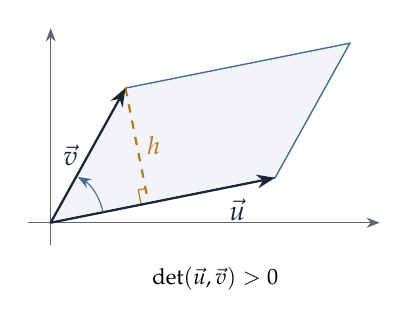
\begin{tikzpicture}[scale=0.95,>=Stealth]
  \draw[->,Gris] (-0.3,0)--(4.4,0); \draw[->,Gris] (0,-0.3)--(0,2.6);
  \fill[Fond,draw=BleuMoyen,line width=0.5pt] (0,0)--(3,0.6)--(4,2.4)--(1,1.8)--cycle;
  \draw[Ocre,dashed,line width=0.8pt] (1,1.8)--(1.3077,0.2615) node[midway,right,font=\small]{$h$};
  \draw[Ocre,line width=0.4pt] (1.2097,0.2419)--(1.1707,0.4380)--(1.2687,0.4576);
  \draw[->,thick,Ink] (0,0)--(3,0.6) node[pos=0.75,below right]{$\ve u$};
  \draw[->,thick,Ink] (0,0)--(1,1.8) node[midway,left]{$\ve v$};
  \draw[->,BleuMoyen] (0.7,0.14) arc (11:60:0.7);
  \node[font=\footnotesize\sffamily,align=center] at (2.2,-0.75) {$\det(\ve u,\ve v)>0$};
\end{tikzpicture}\hfill
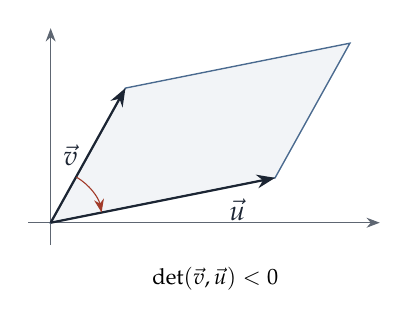
\begin{tikzpicture}[scale=0.95,>=Stealth]
  \draw[->,Gris] (-0.3,0)--(4.4,0); \draw[->,Gris] (0,-0.3)--(0,2.6);
  \fill[Fond,draw=BleuMoyen,line width=0.5pt] (0,0)--(3,0.6)--(4,2.4)--(1,1.8)--cycle;
  \draw[->,thick,Ink] (0,0)--(1,1.8) node[midway,left]{$\ve v$};
  \draw[->,thick,Ink] (0,0)--(3,0.6) node[pos=0.75,below right]{$\ve u$};
  \draw[->,Brique] (0.7*0.4903,0.7*0.8716) arc (60:11:0.7);
  \node[font=\footnotesize\sffamily] at (2.2,-0.75) {$\det(\ve v,\ve u)<0$};
\end{tikzpicture}\hfill
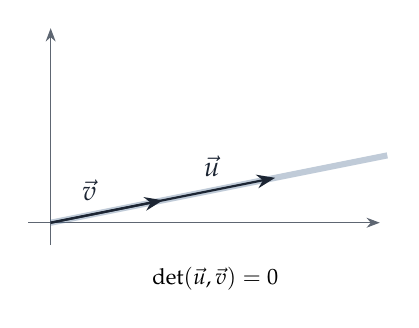
\begin{tikzpicture}[scale=0.95,>=Stealth]
  \draw[->,Gris] (-0.3,0)--(4.4,0); \draw[->,Gris] (0,-0.3)--(0,2.6);
  \draw[BleuMoyen,line width=2.2pt,opacity=0.35] (0,0)--(4.5,0.9);
  \draw[->,thick,Ink] (0,0)--(3,0.6) node[pos=0.8,above left]{$\ve u$};
  \draw[->,thick,Ink] (0,0)--(1.5,0.3) node[midway,above left]{$\ve v$};
  \node[font=\footnotesize\sffamily] at (2.2,-0.75) {$\det(\ve u,\ve v)=0$};
\end{tikzpicture}
\caption{Aire orientée. À gauche, $\ve u$ et $\ve v$ dans le sens direct ; au centre, les mêmes vecteurs dans l'ordre inverse ;
à droite, deux vecteurs colinéaires.}\label{fig:aire2}
\end{figure}

\begin{proposition}\label{prop:col}
$\det(\ve u,\ve v)=0\iff(\ve u,\ve v)$ est liée. Si $ad-bc\neq0$,
$\begin{pmatrix}a&b\\c&d\end{pmatrix}^{-1}=\dfrac1{ad-bc}\begin{pmatrix}d&-b\\-c&a\end{pmatrix}$ (on échange la diagonale, on
change le signe du reste, on divise par le déterminant).
\end{proposition}

En dimension 3, le déterminant de $(\ve u,\ve v,\ve w)$ est le \emph{produit mixte} :
\begin{equation}\label{eq:det3}
\det(\ve u,\ve v,\ve w)=\dt{a&d&g\\b&e&h\\c&f&i}=(\ve u\wedge\ve v)\cdot\ve w
=a\dt{e&h\\f&i}-b\dt{d&g\\f&i}+c\dt{d&g\\e&h}.
\end{equation}
(En pratique, règle de Sarrus : $aei+dhc+gbf-ceg-fha-ibd$.) C'est le \emph{volume orienté} du parallélépipède construit sur les trois vecteurs : aire de la base
$\|\ve u\wedge\ve v\|$ fois hauteur $h=\pm\ve w\cdot\frac{\ve u\wedge\ve v}{\|\ve u\wedge\ve v\|}$. Il est nul si et seulement
si les trois vecteurs sont coplanaires (liés).

\begin{figure}[H]
\centering
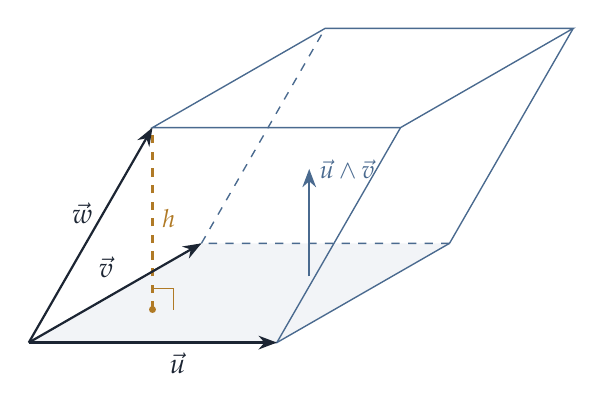
\begin{tikzpicture}[scale=1.05,>=Stealth,x={(1cm,0cm)},y={(0.62cm,0.5cm)},z={(0cm,1cm)}]
  \coordinate (O) at (0,0,0); \coordinate (U) at (3,0,0); \coordinate (V) at (0.6,2.4,0); \coordinate (W) at (1,0.8,2.2);
  \coordinate (UV) at (3.6,2.4,0); \coordinate (UW) at (4,0.8,2.2); \coordinate (VW) at (1.6,3.2,2.2); \coordinate (UVW) at (4.6,3.2,2.2);
  % base
  \fill[Fond] (O)--(U)--(UV)--(V)--cycle;
  \draw[BleuMoyen,line width=0.5pt] (O)--(U)--(UV);
  \draw[BleuMoyen,line width=0.5pt,dashed] (UV)--(V)--(O);
  % arêtes latérales et face supérieure
  \draw[BleuMoyen,line width=0.5pt] (U)--(UW) (UV)--(UVW);
  \draw[BleuMoyen,line width=0.5pt,dashed] (V)--(VW);
  \draw[BleuMoyen,line width=0.5pt] (W)--(UW)--(UVW)--(VW)--cycle;
  % hauteur
  \coordinate (Wp) at (1,0.8,0);
  \draw[Ocre,dashed,line width=0.9pt] (Wp)--(W);
  \node[Ocre,font=\small,right] at (1,0.8,1.1) {$h$};
  \draw[Ocre,line width=0.4pt] (1.25,0.8,0)--(1.25,0.8,0.25)--(1,0.8,0.25);
  \fill[Ocre] (Wp) circle (1.2pt);
  % normale
  \draw[->,thick,BleuMoyen] (2.4,1.6,0)--(2.4,1.6,1.3) node[right,font=\small]{$\ve u\wedge\ve v$};
  % vecteurs
  \draw[->,thick,Ink] (O)--(U) node[pos=0.6,below]{$\ve u$};
  \draw[->,thick,Ink] (O)--(V) node[pos=0.55,above left]{$\ve v$};
  \draw[->,thick,Ink] (O)--(W) node[pos=0.6,left]{$\ve w$};
\end{tikzpicture}\hspace{0.8cm}
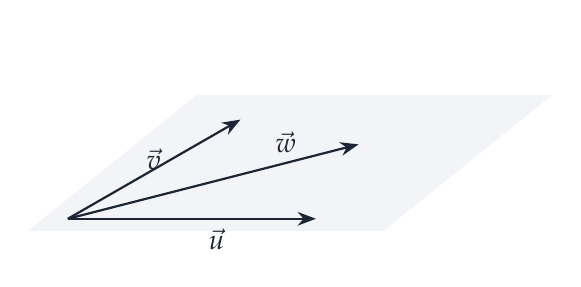
\begin{tikzpicture}[scale=1.05,>=Stealth,x={(1cm,0cm)},y={(0.62cm,0.5cm)},z={(0cm,1cm)}]
  \fill[Fond] (-0.3,-0.3,0)--(4,-0.3,0)--(4,3,0)--(-0.3,3,0)--cycle;
  \draw[->,thick,Ink] (0,0,0)--(3,0,0) node[pos=0.6,below]{$\ve u$};
  \draw[->,thick,Ink] (0,0,0)--(0.6,2.4,0) node[pos=0.6,left]{$\ve v$};
  \draw[->,thick,Ink] (0,0,0)--(2.4,1.8,0) node[pos=0.75,above]{$\ve w$};
  \node at (0,0,2.2) {};
\end{tikzpicture}
\caption{À gauche, le parallélépipède construit sur $\ve u,\ve v,\ve w$, de base grisée (aire $\|\ve u\wedge\ve v\|$) et de hauteur $h$ ; à droite, trois vecteurs coplanaires : $\ve w$ est dans le plan de $\ve u$ et $\ve v$.}\label{fig:volume}
\end{figure}

% ---------------------------------------------------------------------
\subsection{Le déterminant d'ordre $n$}


Les propriétés de l'aire et du volume orientés (§1.1) deviennent la définition en dimension $n$. On note
$C_1,\dots,C_n$ les colonnes de $A$ et l'on écrit $\det A=\det(C_1,\dots,C_n)$.

\begin{theoreme}[définition du déterminant]\label{thm:def}
Il existe une unique application $\det:\Mn{\K}\to\K$ vérifiant :
\begin{enumerate}
\item[(i)] \emph{linéarité par rapport à chaque colonne}, les autres étant fixées :
      $\det(\dots,\lambda C_j+\mu C'_j,\dots)=\lambda\det(\dots,C_j,\dots)+\mu\det(\dots,C'_j,\dots)$ ;
\item[(ii)] \emph{antisymétrie} : échanger deux colonnes change le déterminant en son opposé ;
\item[(iii)] \emph{normalisation} : $\det(I_n)=1$.
\end{enumerate}
\end{theoreme}

\emph{Lecture} (démonstration hors programme pour $n\geq4$). (i) : on peut \emph{sortir un facteur} d'une colonne et
\emph{découper} une colonne en somme --- une aire double si l'on double un côté ; (ii) : l'orientation s'inverse quand on
échange deux vecteurs ; (iii) : le cube unité a pour volume $1$. Pour $n\in\{2,3\}$, c'est le déterminant du §1.1, donc le
produit mixte ; pour $n=2$, (i), (ii), (iii) suffisent à retrouver
$\det\big(ae_1+ce_2,be_1+de_2\big)=ab\det(e_1,e_1)+ad\det(e_1,e_2)+cb\det(e_2,e_1)+cd\det(e_2,e_2)=ad-bc$, car $\det(e_1,e_1)=\det(e_2,e_2)=0$ (ii) et $\det(e_2,e_1)=-\det(e_1,e_2)=-1$.

\begin{theoreme}[développement]\label{thm:dev}
Pour tous $i,j$ (démonstration non exigible) :
\[\det A=\sum_{j=1}^n(-1)^{i+j}a_{i,j}\Delta_{i,j}\quad\text{(ligne $i$)},\qquad
\det A=\sum_{i=1}^n(-1)^{i+j}a_{i,j}\Delta_{i,j}\quad\text{(colonne $j$)},\]
où le \emph{mineur} $\Delta_{i,j}$ est le déterminant obtenu en supprimant la ligne $i$ et la colonne $j$, les signes
$(-1)^{i+j}$ formant un damier qui commence par $+$. Tout ce qui est vrai des colonnes est vrai des lignes
($\det A^T=\det A$).
\end{theoreme}

Le développement donne une définition équivalente, \emph{par récurrence} sur $n$ à partir de $\dt{a&b\\c&d}=ad-bc$ ; pour
$n=3$, on retrouve~\eqref{eq:det3}.

\begin{proposition}\label{prop:op}
\begin{enumerate}
\item Une colonne nulle, ou deux colonnes égales (ou proportionnelles) : $\det A=0$.
\item $\det(\lambda A)=\lambda^n\det A$ \quad (on sort $\lambda$ de chacune des $n$ colonnes).
\item Échange $C_i\leftrightarrow C_j$ : le signe change. Dilatation $C_i\leftarrow\lambda C_i$ : $\det$ est multiplié
      par $\lambda$. Transvection $C_i\leftarrow C_i+\lambda C_j$ ($j\neq i$) : $\det$ \emph{ne change pas}.
\end{enumerate}
\end{proposition}

\begin{proof}
Tout découle de la définition. Deux colonnes égales : les échanger ne change pas $A$ mais change le signe (ii), donc
$\det A=-\det A=0$ ; une colonne nulle s'écrit $0\cdot C$ (i). Point 2 : (i) appliquée à chacune des $n$ colonnes. Échange :
(ii) ; dilatation : (i). Transvection : par (i), $\det(\dots,C_i+\lambda C_j,\dots)=\det A+\lambda\det(\dots,C_j,\dots,C_j,\dots)=\det A$.
\end{proof}

\begin{attention}
$\det(A+B)\neq\det A+\det B$ et $\det(\lambda A)=\lambda^n\det A$, non $\lambda\det A$. Dans une transvection, la colonne
modifiée garde le coefficient $1$ ; deux opérations successives s'appliquent l'une \emph{après} l'autre (la seconde voit la
colonne déjà modifiée).
\end{attention}

\begin{theoreme}\label{thm:tri}
Le déterminant d'une matrice triangulaire est le produit de ses coefficients diagonaux.
\end{theoreme}

\begin{proof}
Par récurrence sur $n$. Si $T$ est triangulaire supérieure, sa dernière ligne vaut $(0,\dots,0,t_{n,n})$ ; en développant
selon elle, $\det T=(-1)^{n+n}t_{n,n}\Delta_{n,n}$, et $\Delta_{n,n}$ est triangulaire de diagonale
$t_{1,1},\dots,t_{n-1,n-1}$.
\end{proof}

\begin{methode}{Calculer un déterminant}\label{meth:calcul}
\begin{enumerate}
\item \emph{Regarder avant de calculer} : colonnes liées ? somme constante sur les lignes ? ligne ou colonne presque nulle ?
      structure (tridiagonale, puissances, formule en $i,j$) ? La section~\ref{sec:techniques} donne la méthode pour chaque
      structure.
\item Sinon, \emph{pivot de Gauss} : créer des zéros par transvections (en notant les échanges et les facteurs sortis)
      jusqu'à une forme triangulaire, ou jusqu'à une ligne ou colonne n'ayant qu'un coefficient non nul, selon laquelle on
      développe.
\item Avec un paramètre, \emph{garder les facteurs} : on sort tout facteur commun dès qu'il apparaît ; une forme développée
      ne se refactorise presque jamais.
\end{enumerate}
\end{methode}

\begin{exemple}[choisir la méthode]
\[D=\dt{1&2&3&4\\4&1&2&3\\3&4&1&2\\2&3&4&1}.\]
Le pivot aboutit, mais au prix de calculs où l'on se trompe facilement. Plus vite : chaque ligne a pour somme $10$. $C_1\leftarrow C_1+C_2+C_3+C_4$ puis on sort $10$ ; $L_i\leftarrow L_i-L_1$ :
\[D=10\dt{1&2&3&4\\1&1&2&3\\1&4&1&2\\1&3&4&1}=10\dt{-1&-1&-1\\2&-2&-2\\1&1&-3}=10\times(-16)=-160.\]
(Dans le $3\times3$, $C_2\leftarrow C_2-C_1$ et $C_3\leftarrow C_3-C_1$ donnent $\dt{-1&0&0\\2&-4&-4\\1&0&-4}=-16$.)
\end{exemple}

% ---------------------------------------------------------------------
\subsection{Propriétés globales}

\begin{theoreme}\label{thm:fond}
Soient $A,B\in\Mn{\K}$.
\begin{enumerate}
\item $A$ est inversible $\iff\det A\neq0\iff$ les colonnes de $A$ sont libres.
\item $\det(AB)=\det A\det B$ ; si $A$ est inversible, $\det(A^{-1})=\frac1{\det A}$ ; $\det(A^T)=\det A$.
\item Deux matrices semblables ont même déterminant : $\det(PBP^{-1})=\det P\det B\det P^{-1}=\det B$.
\end{enumerate}
\end{theoreme}

\begin{proof}
Si les colonnes sont liées, $C_i=\sum_{j\neq i}\lambda_jC_j$, la transvection $C_i\leftarrow C_i-\sum_{j\neq i}\lambda_jC_j$ rend
une colonne nulle : $\det A=0$. Si $A$ est inversible, $\det A\det A^{-1}=\det I_n=1$. (Produit et transposée : admis.)
\end{proof}

\begin{definition}
Si $E$ est de dimension $n$, de base $\mathcal B$ : $\det_{\mathcal B}(u_1,\dots,u_n)$ est le déterminant de la matrice des
coordonnées des $u_j$ dans $\mathcal B$ ; pour $f\in\LE$, $\det f=\det\Mat_{\mathcal B}(f)$, indépendant de $\mathcal B$
(matrices semblables).
\end{definition}

\begin{theoreme}\label{thm:base}
$(u_1,\dots,u_n)$ est une base de $E\iff\det_{\mathcal B}(u_1,\dots,u_n)\neq0$. $f$ est un automorphisme $\iff\det f\neq0$.
Enfin $\det(f\circ g)=\det f\det g$, $\det(\lambda f)=\lambda^n\det f$, $\det(f^{-1})=\frac1{\det f}$, $\det\Id=1$.
\end{theoreme}

Par exemple, $(1,1+X,\dots,1+X+\dots+X^n)$ est une base de $\R_n[X]$ (matrice triangulaire à diagonale de $1$), et la
dérivation $D$ de $\R_n[X]$ vérifie $\det D=0$ (matrice triangulaire à diagonale nulle) : elle n'est pas bijective.

\begin{reflexe}
Pour un endomorphisme défini géométriquement, on calcule $\det f$ dans la base où sa matrice est la plus simple (base
adaptée), jamais dans la base canonique.
\end{reflexe}

\begin{proposition}\label{prop:proj-sym}
Soit $E$ de dimension $n$. Un projecteur $p$ vérifie $\det p=1$ si $p=\Id$, $\det p=0$ sinon. Une symétrie $s$ vérifie
$\det s=(-1)^{\dim\mathrm{Ker}(s+\Id)}=(-1)^{n-\rg(s+\Id)}$.
\end{proposition}

\begin{proof}
Dans une base adaptée à $E=\mathrm{Im}\,p\oplus\mathrm{Ker}\,p$, $\Mat(p)=\mathrm{diag}(I_r,0)$. Dans une base adaptée à
$E=\mathrm{Ker}(s-\Id)\oplus\mathrm{Ker}(s+\Id)$, $\Mat(s)=\mathrm{diag}(I_r,-I_{n-r})$ ; et $\frac12(s+\Id)$ est le
projecteur sur $\mathrm{Ker}(s-\Id)$, donc $\rg(s+\Id)=r$.
\end{proof}

\begin{horsprogramme}\phantomsection\label{hp:comatrice}
\textbf{Comatrice.} La comatrice $\mathrm{com}(A)$ est la matrice des cofacteurs $(-1)^{i+j}\Delta_{i,j}$. Pour toute $A$,
$A\,\mathrm{com}(A)^T=\mathrm{com}(A)^TA=\det(A)\,I_n$, donc $A^{-1}=\frac1{\det A}\mathrm{com}(A)^T$ si $\det A\neq0$.
\emph{Pourquoi} : le coefficient $(i,i)$ de $A\,\mathrm{com}(A)^T$ est le développement de $\det A$ selon la ligne $i$ ; le
coefficient $(k,i)$, $k\neq i$, est le développement selon la ligne $i$ de la matrice où la ligne $i$ est remplacée par la
ligne $k$ : deux lignes égales, donc $0$. Utile en taille $2$ ou $3$ et pour les questions théoriques ; au-delà, le pivot
est plus rapide.
\end{horsprogramme}

\begin{exo}{td-d8}{3}{\TD{8}similitude \HP}
Soit $\C$ vu comme un $\R$-espace vectoriel. On fixe $a\in\C^*$ et l'on note $f(z)=az$, appelée similitude linéaire de
rapport $a$ dans le plan complexe.
\begin{enumerate}
\item Prouver que $f$ est bijective et déterminer $f^{-1}$.
\item À quelle condition $f$ est-elle une symétrie du plan ?
\item Calculer $\mathrm{tr}(f)$ et $\det(f)$ en fonction de $a$.
\item Si $|a|=1$, reconnaître $f$ en tant qu'application géométrique simple.
\end{enumerate}
\end{exo}
\begin{exo}{g-carre}{3}{multiplicativité ; propriété globale}
Soit $A\in\Mn{\R}$ telle que $A^2=-I_n$. Montrer que $n$ est pair. Le résultat subsiste-t-il pour une matrice complexe ?
\end{exo}
\begin{exo}{b-endo}{4}{déterminant d'un endomorphisme de matrices}
Soit $A=\begin{pmatrix}a&b\\c&d\end{pmatrix}$ et $f:\mathcal M_2(\R)\to\mathcal M_2(\R)$, $M\mapsto AM$. Montrer que
$\det f=(\det A)^2$. En déduire une condition pour que $f$ soit bijectif, et $f^{-1}$.
\end{exo}
\begin{exo}{hp-com}{3}{comatrice, coefficients entiers \HP}
\begin{enumerate}
\item Calculer la comatrice de $A=\begin{pmatrix}1&2&0\\0&1&1\\1&0&1\end{pmatrix}$ et en déduire $A^{-1}$.
\item Soit $A$ à coefficients entiers. Montrer que $A$ est inversible d'inverse à coefficients entiers si et seulement si
      $\det A=\pm1$.
\item Pour $A$ inversible, exprimer $\det(\mathrm{com}A)$ en fonction de $\det A$.
\end{enumerate}
\end{exo}

% ---------------------------------------------------------------------
\subsection{Géométrie : alignement, distances}

Le déterminant traduit directement l'alignement et la coplanarité :
$A,B,C$ alignés $\iff\det(\vv{AB},\vv{AC})=0$ ; $M\in(ABC)\iff\det(\vv{AM},\vv{AB},\vv{AC})=0$ ; aire du triangle
$=\frac12|\det(\vv{AB},\vv{AC})|$ ; volume du tétraèdre $=\frac16|\det(\vv{AB},\vv{AC},\vv{AD})|$ (base orthonormée).

\begin{proposition}\label{prop:dist-droites}
Soient $\mathcal D_1=A+\vect(\ve u)$ et $\mathcal D_2=C+\vect(\ve v)$ non parallèles. Il existe un unique couple
$(H,K)\in\mathcal D_1\times\mathcal D_2$ avec $(HK)$ perpendiculaire aux deux droites, et
\[d(\mathcal D_1,\mathcal D_2)=HK=\frac{|\det(\vv{AC},\ve u,\ve v)|}{\|\ve u\wedge\ve v\|}.\]
\end{proposition}

\begin{figure}[H]
\centering
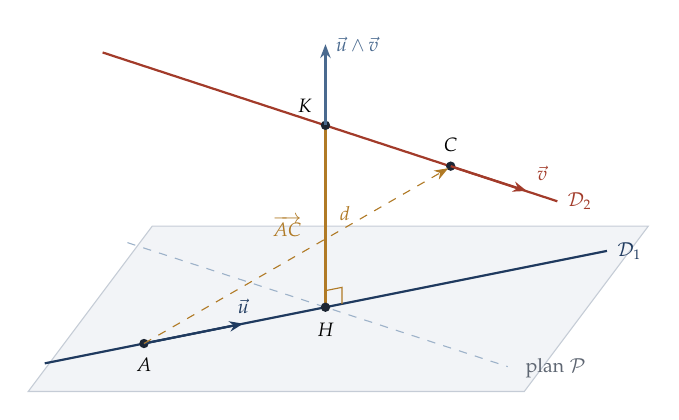
\begin{tikzpicture}[scale=1.05,>={Stealth[length=5pt]}]
\fill[Fond] (0,0)--(6,0)--(7.5,2)--(1.5,2)--cycle;
\draw[Filet] (0,0)--(6,0)--(7.5,2)--(1.5,2)--cycle;
\node[font=\scriptsize,Gris,anchor=south west] at (5.9,0.05) {plan $\mathcal P$};
% D1 dans le plan
\draw[Bleu,thick] (0.2,0.34)--(7.0,1.70) node[right,font=\scriptsize]{$\mathcal D_1$};
% projection de D2 dans le plan
\draw[BleuClair,dashed] (1.2,1.8)--(5.8,0.3);
% D2 au-dessus
\draw[Brique,thick] (0.9,4.1)--(6.4,2.3) node[right,font=\scriptsize]{$\mathcal D_2$};
% perpendiculaire commune
\draw[Ocre,thick] (3.595,1.019)--(3.595,3.219);
\draw[Ocre] (3.595,1.219)--(3.795,1.259)--(3.795,1.059);
\node[pt] at (3.595,1.019) {}; \node[font=\scriptsize,anchor=north] at (3.595,0.95) {$H$};
\node[pt] at (3.595,3.219) {}; \node[font=\scriptsize,anchor=south east] at (3.55,3.25) {$K$};
\node[font=\scriptsize,Ocre,anchor=west] at (3.65,2.15) {$d$};
% A, C et vecteurs
\node[pt] at (1.4,0.58) {}; \node[font=\scriptsize,anchor=north] at (1.4,0.52) {$A$};
\draw[->,Bleu,thick] (1.4,0.58)--(2.6,0.82) node[above,font=\scriptsize]{$\ve u$};
\node[pt] at (5.11,2.725) {}; \node[font=\scriptsize,anchor=south] at (5.11,2.78) {$C$};
\draw[->,Brique,thick] (5.11,2.725)--(6.03,2.425) node[above right,font=\scriptsize]{$\ve v$};
\draw[->,Ocre,dashed] (1.4,0.58)--(5.08,2.70) node[pos=0.55,above left,font=\scriptsize]{$\vv{AC}$};
\draw[->,BleuMoyen,thick] (3.595,3.219)--(3.595,4.2) node[right,font=\scriptsize]{$\ve u\wedge\ve v$};
\end{tikzpicture}
\caption{Deux droites non coplanaires, le plan $\mathcal P$ contenant $\mathcal D_1$ et parallèle à $\mathcal D_2$ (gris),
et la perpendiculaire commune $[HK]$ (ocre).}\label{fig:dist-droites}
\end{figure}

\emph{Lecture.} Le plan gris contient $\mathcal D_1$ et est parallèle à $\mathcal D_2$ ; la distance est la hauteur de
$\mathcal D_2$ au-dessus de ce plan. Or $|\det(\vv{AC},\ve u,\ve v)|$ est le volume du parallélépipède de base
$\|\ve u\wedge\ve v\|$ et de hauteur $d$ : on divise le volume par la base. La démonstration fait l'objet du TD~2.

\begin{exo}{td-d1}{2}{\TD{1}alignement}
Soit $A(a,a')$, $B(b,b')$ et $C(c,c')$ tels que $\dt{1&1&1\\a&b&c\\a'&b'&c'}=0$. Montrer que $A$, $B$, $C$ sont alignés dans
le plan.
\end{exo}
\begin{exo}{td-d2}{3}{\TD{2}distance de deux droites}
Soient $(AB)$ et $(CD)$ deux droites (non parallèles) de l'espace. Prouver que
\[d\big((AB),(CD)\big)=\frac{\big|\det(\vv{AB},\vv{CD},\vv{AC})\big|}{\|\vv{AB}\wedge\vv{CD}\|}.\]
\end{exo}

% ---------------------------------------------------------------------
\subsection{Techniques de calcul d'ordre $n$}\label{sec:techniques}

\subsubsection{Somme constante}

\begin{proposition}\label{prop:ab}
Le déterminant d'ordre $n$ à diagonale $a$ et autres coefficients $b$ vaut $D_n(a,b)=\big(a+(n-1)b\big)(a-b)^{n-1}$.
\end{proposition}

\begin{proof}
Chaque ligne a pour somme $s=a+(n-1)b$. $C_1\leftarrow C_1+\dots+C_n$ remplit la première colonne de $s$, que l'on sort ;
$L_i\leftarrow L_i-L_1$ ($i\geq2$) laisse une matrice triangulaire de diagonale $(1,a-b,\dots,a-b)$.
\end{proof}

\begin{exo}{td-d6}{3}{\TD{6}base et déterminant}
Soit $\mathcal B=(e_1,\dots,e_n)$ une base d'un espace vectoriel $E$ sur $\K$, et $(a,b)\in\K^2$. On pose, pour
$j\in\ient1n$, $\delta_j=ae_j+b\sum_{i\neq j}e_i$. Prouver que $\mathcal C=(\delta_1,\dots,\delta_n)$ est une base de $E$ si et
seulement si $a\neq b$ et $a+(n-1)b\neq0$.
\end{exo}

\subsubsection{Matrices définies par une formule : différences successives}

\begin{methode}{Différences successives}\label{meth:diff}
Si deux colonnes voisines se ressemblent ($a_{i,j}=\max(i,j)$, $|i-j|$, $a^{|i-j|}$\dots), on effectue
$C_k\leftarrow C_k-C_{k-1}$ (ou $C_k-aC_{k-1}$) \emph{pour $k$ allant de $n$ à $2$} --- en commençant par la fin, chaque
opération utilise une colonne intacte. On calcule le nouveau coefficient en distinguant $i<k$ et $i\geq k$ : on obtient des
blocs de $0$ et de $\pm1$, puis une matrice triangulaire ou une ligne creuse.
\end{methode}

\begin{exemple}\label{ex:max}
$A_n=\big(\max(i,j)\big)$. Après $C_k\leftarrow C_k-C_{k-1}$ ($k=n,\dots,2$), le coefficient $(i,k)$ vaut
$\max(i,k)-\max(i,k-1)=1$ si $i<k$, $0$ si $i\geq k$ ; la première colonne reste $(1,\dots,n)^T$. La dernière ligne devient
$(n,0,\dots,0)$ : en développant selon elle, $\det A_n=(-1)^{n+1}n\,\Delta_{n,1}$, avec $\Delta_{n,1}$ triangulaire à
diagonale de $1$. Donc $\det A_n=(-1)^{n+1}n$.
\end{exemple}

\begin{exo}{f-absij}{4}{différences de colonnes puis de lignes}
Calculer le déterminant $B_n$ de la matrice $\big(|i-j|\big)_{1\leq i,j\leq n}$, $n\geq2$.
\end{exo}
\begin{exo}{f-ka}{4}{différences pondérées}
Soit $a\in\R$. Calculer $\det\big(a^{|i-j|}\big)_{1\leq i,j\leq n}$.
\end{exo}

\subsubsection{Déterminants creux}

\begin{reflexe}
Une ligne (ou colonne) n'ayant qu'\emph{un} coefficient non nul : on développe selon elle, avec le signe $(-1)^{i+j}$. Deux
coefficients non nuls : on développe et les deux mineurs ont souvent la forme de départ, d'où une récurrence.
\end{reflexe}

\begin{astuce}
Permuter les lignes \emph{et} les colonnes par la \emph{même} permutation ne change pas le déterminant (les signes se
compensent ; c'est $\det(P^{-1}AP)=\det A$). On regroupe ainsi les coefficients non nuls en blocs diagonaux.
\end{astuce}

\begin{exo}{td-d4}{3}{\TD{4}déterminant en forme de X}
Pour $(a,b)\in\K^2$, calculer le déterminant de taille $2n\times2n$
\[A_{2n}=\dt{a&0&\cdots&\cdots&0&b\\0&a&&&b&0\\\vdots&&\ddots&\iddots&&\vdots\\\vdots&&\iddots&\ddots&&\vdots\\0&b&&&a&0\\b&0&\cdots&\cdots&0&a}.\]
\end{exo}
\begin{exo}{td-d9}{4}{\TD{9}déterminant en forme de Z}
Soit $n\geq3$. On considère le déterminant en forme de Z
\[D=\dt{a_1&a_2&\cdots&a_{n-1}&a_n\\0&0&\cdots&b_{n-1}&0\\\vdots&&\iddots&&\vdots\\0&b_2&\cdots&0&0\\c_1&c_2&\cdots&c_{n-1}&c_n},\]
où, pour $2\leq k\leq n-1$, la ligne $k$ ne contient que $b_{n+1-k}$, en colonne $n+1-k$. Calculer $\det(D)$ en pensant d'abord
à factoriser tout ce qui peut l'être.
\end{exo}

\subsubsection{Déterminant de Vandermonde}

\begin{theoreme}\label{thm:vdm}
$V(x_1,\dots,x_n)=\det\big(x_j^{\,i-1}\big)_{1\leq i,j\leq n}=\prod_{1\leq i<j\leq n}(x_j-x_i)$, non nul si et seulement si les
$x_i$ sont deux à deux distincts.
\end{theoreme}

\begin{methode}{Voir un déterminant comme un polynôme}\label{meth:poly}
Si une variable $x$ n'apparaît que dans une colonne, le développement selon cette colonne montre que $P(x)$ est un
polynôme, de coefficient dominant un cofacteur. On cherche ses racines évidentes (valeurs rendant deux colonnes
égales) ; si l'on en trouve autant que le degré, $P$ est le coefficient dominant fois le produit des $(x-\text{racine})$.
Démonstration du théorème : TD~5.
\end{methode}

\begin{exo}{td-d5}{4}{\TD{5}déterminant de Vandermonde}
Soit $A=\begin{pmatrix}1&1&1&1\\a&b&c&x\\a^2&b^2&c^2&x^2\\a^3&b^3&c^3&x^3\end{pmatrix}$ et $P(x)=\det(A)$.
\begin{enumerate}
\item Prouver que $P$ est un polynôme, donner son degré et ses racines.
\item En déduire la valeur de $\det(A)$ sous forme de produit de $6$ facteurs.
\item Soit $A=\big(a_j^{\,i-1}\big)_{1\leq i,j\leq n}$ ; montrer par récurrence que
      $\det(A)=\prod_{k=2}^n\prod_{p=1}^{k-1}(a_k-a_p)$.
\end{enumerate}
\end{exo}

\subsubsection{Déterminants tridiagonaux : récurrences}

\begin{methode}{Établir et résoudre une récurrence}\label{meth:rec}
Développer selon la première ligne, puis développer le second mineur selon sa première colonne : pour un tridiagonal de
diagonale $a$, de sur-diagonale $b$ et de sous-diagonale $c$ (constantes), $T_n=aT_{n-1}-bc\,T_{n-2}$. Seul le
\emph{produit} $bc$ compte. On résout avec l'équation caractéristique $r^2=ar-bc$ :
\begin{itemize}
\item deux racines distinctes $r_1,r_2$ (réelles ou complexes) : $T_n=\lambda r_1^n+\mu r_2^n$ ;
\item racine double $r$ : $T_n=(\lambda+\mu n)r^n$ ;
\item racines $e^{\pm i\theta}$ : $T_n=\lambda\cos n\theta+\mu\sin n\theta$.
\end{itemize}
On fixe $\lambda,\mu$ avec $T_1$, $T_2$ (ou $T_0=1$, valeur compatible avec la relation), et l'on vérifie $T_3$.
\end{methode}

\begin{exo}{td-d3}{3}{\TD{3}suite récurrente linéaire d'ordre 2}
Soit $A_n=\big(5\delta_{i,j}+6\delta_{i,j-1}+\delta_{i-1,j}\big)_{1\leq i,j\leq n}$.
\begin{enumerate}
\item Calculer $\det(A_4)$.
\item Soit $u_n=\det(A_n)$. Montrer que $(u_n)$ est une suite récurrente linéaire d'ordre 2 et la calculer.
\end{enumerate}
\end{exo}
\begin{exo}{td-d7}{4}{\TD{7}suite récurrente, racines complexes}
Soit $\theta\in\R$. On considère la matrice d'ordre $n$ ayant des $2\cos\theta$ sur la diagonale, des $1$ juste au-dessus et
juste au-dessous, et des $0$ ailleurs. Vérifier que $\det(A_n)=\dfrac{\sin\big((n+1)\theta\big)}{\sin\theta}$.
\end{exo}

\subsubsection{Ajouter une constante à tous les coefficients}

\begin{methode}{Fonction affine}\label{meth:affine}
Si $D(x)$ est le déterminant obtenu en ajoutant $x$ à tous les coefficients, les opérations $C_j\leftarrow C_j-C_1$
($j\geq2$) chassent $x$ de toutes les colonnes sauf la première ; par linéarité, $x\mapsto D(x)$ est \emph{affine}. On la
détermine par deux valeurs de $x$ qui rendent la matrice triangulaire.
\end{methode}

\begin{exo}{td-d10}{5}{\TD{10}polynôme de degré 1}
On note $U$ la matrice de taille $n\times n$ dont tous les coefficients valent $1$, et
\[A_n=\begin{pmatrix}\lambda_1&a&\cdots&a\\b&\lambda_2&\ddots&\vdots\\\vdots&\ddots&\ddots&a\\b&\cdots&b&\lambda_n\end{pmatrix}.\]
\begin{enumerate}
\item Soit $P(x)=\det(A_n-xU)$. Montrer que $\deg(P)\leq1$.
\item Calculer $P(a)$ et $P(b)$ et en déduire $\det(A_n)$ pour $a\neq b$.
\item À l'aide d'une dérivée, trouver $\det(A_n)$ pour $a=b$.
\end{enumerate}
\end{exo}
\begin{exo}{det-pb}{4}{fonction affine, parité, antisymétrie}
Soit $M_n(x)$ la matrice d'ordre $n\geq2$ ayant des $x$ sur la diagonale, des $1$ au-dessus et des $-1$ au-dessous.
\begin{enumerate}
\item Montrer que $\det M_n(x)=\dfrac{(x+1)^n+(x-1)^n}2$.
\item Pour quelles valeurs réelles de $x$ la matrice est-elle inversible ?
\end{enumerate}
\end{exo}

\begin{essentiel}
\small
\begin{tabular}{>{\raggedright}p{0.44\linewidth}p{0.48\linewidth}}
Structure repérée & Méthode\\\midrule
colonnes liées, rang $\leq2$ & $\det=0$ sans calcul\\
même somme sur chaque ligne & $C_1\leftarrow\sum C_j$, sortir la somme\\
$a_{i,j}$ donné par une formule ($\max$, $|i-j|$) & différences $C_k-C_{k-1}$ de $k=n$ à $2$\\
lignes à un ou deux coefficients (X, Z, N) & développer ; permuter lignes et colonnes ensemble\\
puissances successives & Vandermonde, ou polynôme en $x$\\
tridiagonal & récurrence d'ordre 2\\
constante ajoutée partout, $a$ au-dessus, $b$ au-dessous & fonction affine, cas $a=b$ par dérivée\\
relation entre matrices ($A^2=-I$, $A^T=-A$) & $\det(AB)$, $\det(\lambda A)$, $\det A^T$\\
endomorphisme géométrique & base adaptée
\end{tabular}
\end{essentiel}
% =====================================================================
%                 CHAPITRE 2 — COURBES PARAMÉTRÉES PLANES
% =====================================================================
\clearpage
\section{Courbes paramétrées planes}\label{sec:courbes}

Une courbe n'a pas toujours d'équation $y=g(x)$ : à une abscisse peuvent correspondre plusieurs points (un cercle, une
boucle). On la décrit alors par un point mobile $M(t)$. Étudier la courbe, c'est savoir la tracer avec ses points
remarquables, ses tangentes et ses branches infinies ; le chapitre donne les outils, dans l'ordre où ils servent.

% ---------------------------------------------------------------------
\subsection{Représentation paramétrique}

Une \emph{courbe paramétrée} est une application $f:I\to\R^2$ (ou $\R^3$) de classe $\mathcal C^1$,
$t\mapsto f(t)=\vv{OM(t)}=\big(x(t),y(t)\big)$ ; son \emph{support} est $\mathcal C=\{M(t),\ t\in I\}$. On distingue
l'\emph{équation cartésienne} $\mathcal C=\{(x,y)\mid F(x,y)=0\}$ et la \emph{représentation paramétrique} :
\begin{itemize}
\item la droite passant par $A(1,2)$ et $B(2,-2)$ : équation $y=-4x+6$ (par $\det(\vv{AB},\vv{AM})=0$), paramétrage
      $t\mapsto A+t\vv{AB}$ ou $t\mapsto(t,-4t+6)$ ;
\item le cercle de centre $\Omega(1,2)$ et de rayon $R$ : $(x-1)^2+(y-2)^2=R^2$, paramétré par
      $\theta\mapsto(1+R\cos\theta,2+R\sin\theta)$, $\theta\in\,]-\pi,\pi]$ ; son demi-cercle $y\geq2$ est le graphe de
      $x\mapsto2+\sqrt{R^2-(x-1)^2}$ ;
\item un graphe $y=g(x)$ est la courbe $t\mapsto(t,g(t))$.
\end{itemize}

\begin{proposition}[fonctions vectorielles]\label{prop:fv}
Limite, continuité, dérivabilité, classe $\mathcal C^k$ se lisent \emph{sur les coordonnées}, et $f'=(x',y')$ : c'est le
vecteur vitesse ($f''$ : accélération, $\|f'\|$ : vitesse scalaire). Pour $f,g$ dérivables, $\lambda$ scalaire et $\varphi$
réelle :
\[(\lambda f+g)'=\lambda f'+g',\qquad(\varphi f)'=\varphi'f+\varphi f',\qquad(f\circ\varphi)'=\varphi'\,(f'\circ\varphi),\]
\[(f\cdot g)'=f'\cdot g+f\cdot g',\qquad(f\wedge g)'=f'\wedge g+f\wedge g'\ \ (\text{dans }\R^3),\]
et la formule de Leibniz $(\varphi f)^{(n)}=\sum_{k=0}^n\binom nk\varphi^{(k)}f^{(n-k)}$. Taylor--Young (démonstration hors
programme) : $f(t_0+h)=\sum_{k=0}^n\frac{h^k}{k!}f^{(k)}(t_0)+o(h^n)$ ; les développements limités se calculent coordonnée par
coordonnée.
\end{proposition}
Exemple type : si $\|f\|$ est constante, dériver $f\cdot f$ donne $f\cdot f'=0$ ; le mouvement circulaire a une vitesse
orthogonale au rayon.


% ---------------------------------------------------------------------
\subsection{Tangente en un point régulier}

\begin{definition}
La courbe admet une tangente $T$ en $M(t_0)$ si la droite $M(t_0)+\vect(\ve u_h)$, où
$\ve u_h=\frac{\vv{M(t_0)M(t_0+h)}}{\|\vv{M(t_0)M(t_0+h)}\|}$ dirige la corde, a une position limite quand $h\to0$. On
normalise parce que $\vv{M(t_0)M(t_0+h)}\to\ve0$ ne donne, seul, aucune direction. $M(t_0)$ est \emph{régulier} si
$f'(t_0)\neq\ve0$, \emph{stationnaire} sinon ; la courbe est \emph{régulière} si tous ses points le sont. On \emph{oriente} une
courbe régulière en choisissant un sens de parcours, ou le vecteur unitaire tangent $\frac{f'}{\|f'\|}$.
\end{definition}

\begin{figure}[H]
\centering
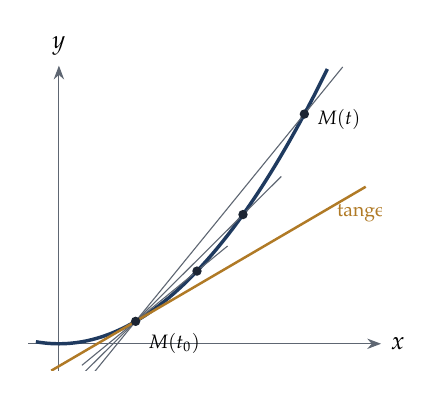
\begin{tikzpicture}
\begin{axis}[courbe,width=0.5\linewidth,xmin=-0.2,xmax=2.1,ymin=-0.3,ymax=3.1,xtick=\empty,ytick=\empty,axis equal image=false,height=0.45\linewidth]
\addplot[arcetude,domain=-0.15:1.75,samples=100]({x},{x^2});
\addplot[Gris,thin,domain=0.15:1.85,samples=2]{0.25+2.1*(x-0.5)};
\addplot[Gris,thin,domain=0.15:1.45,samples=2]{0.25+1.7*(x-0.5)};
\addplot[Gris,thin,domain=0.15:1.1,samples=2]{0.25+1.4*(x-0.5)};
\addplot[tgte,domain=-0.05:2.0,samples=2]{x-0.25};
\node[pt] at (axis cs:0.5,0.25) {}; \node[font=\scriptsize,anchor=north west] at (axis cs:0.52,0.22) {$M(t_0)$};
\node[pt] at (axis cs:1.6,2.56) {}; \node[pt] at (axis cs:1.2,1.44) {}; \node[pt] at (axis cs:0.9,0.81) {};
\node[font=\scriptsize,anchor=west] at (axis cs:1.62,2.5) {$M(t)$};
\node[font=\scriptsize,Ocre,anchor=west] at (axis cs:1.75,1.45) {tangente};
\end{axis}
\end{tikzpicture}
\caption{Sur la parabole $(t,t^2)$, les cordes issues de $M(t_0)$, $t_0=\frac12$, pivotent vers la tangente quand $t\to t_0$.}\label{fig:cordes}
\end{figure}

\begin{theoreme}\label{thm:tgte}
En un point régulier, la tangente est $M(t_0)+\vect\big(f'(t_0)\big)$ ($f'(t_0)$ est un \emph{vecteur tangent} ; c'est
aussi le paramétrage de la tangente dans $\R^3$) ; dans le plan, elle a pour équation
\[\det\big(\vv{M(t_0)M},f'(t_0)\big)=0\iff y'(t_0)\big(x-x(t_0)\big)-x'(t_0)\big(y-y(t_0)\big)=0.\]
On la trace en reportant $f'(t_0)$ depuis $M(t_0)$. Elle est horizontale si $y'(t_0)=0$, verticale si $x'(t_0)=0$.
\end{theoreme}

\begin{proof}
Taylor--Young à l'ordre 1 : $\vv{M(t_0)M(t_0+h)}=h\big(f'(t_0)+o(1)\big)$, donc
$\ve u_h=\frac{h}{|h|}\cdot\frac{f'(t_0)+o(1)}{\|f'(t_0)\|+o(1)}\to\pm\frac{f'(t_0)}{\|f'(t_0)\|}$ selon que $h\to0^\pm$ : les deux
limites dirigent la même droite.
\end{proof}

\paragraph{D'où vient la pente} Si $x'(t_0)\neq0$, $x$ est strictement monotone près de $t_0$ : localement, la courbe est le
graphe d'une fonction $g$, avec $y(t)=g\big(x(t)\big)$. En dérivant la composée, $y'(t)=g'\big(x(t)\big)\,x'(t)$, donc la pente
de la tangente est $g'\big(x(t_0)\big)=\frac{y'(t_0)}{x'(t_0)}$.

\begin{attention}
« $x'(t_0)=0$, donc tangente verticale » n'est vrai que si $y'(t_0)\neq0$. Et ne pas confondre $\frac{y(t)}{x(t)}$, pente de la
droite $\big(OM(t)\big)$, avec la pente $\frac{y'}{x'}$ de la tangente : elles ne se rejoignent qu'à la limite, quand $M(t)\to O$
(la corde issue de $O$ tend vers la tangente en $O$) ; c'est ainsi qu'on obtient la tangente en un point limite $O$.
\end{attention}

% ---------------------------------------------------------------------
\subsection{Plan d'étude et réduction}

\begin{methode}{Étudier une courbe paramétrée}\label{meth:plan-courbe}
\begin{enumerate}
\item \emph{Domaine} : intersection des domaines de $x$ et $y$ ; noter les valeurs interdites (futures branches infinies).
\item \emph{Réduction} : période, puis symétries. On cherche un changement de paramètre $\varphi$ ($t\mapsto-t$, $\pi-t$,
      $\frac1t$\dots) tel que $M(\varphi(t))$ soit l'image de $M(t)$ par une symétrie $s$ ; si $\varphi$ envoie $I'$ sur le reste
      du domaine, on étudie sur $I'$ et l'on complète par $s$.
\item \emph{Dérivées factorisées} : signes de $x'$ et $y'$, points stationnaires (zéros communs), tangentes horizontales et
      verticales.
\item \emph{Tableau conjoint} de $x$ et $y$ avec les valeurs aux points remarquables et les limites.
\item \emph{Points stationnaires} (\S2.4), \emph{branches infinies} (\S2.5), inflexions si demandé ; \emph{points doubles} :
      résoudre $f(t)=f(s)$, $t\neq s$, ou comparer deux arcs écrits comme graphes par le théorème des valeurs intermédiaires
      (TD~1).
\item \emph{Tracé} : asymptotes en pointillés, points avec un petit segment de tangente, arcs suivant le tableau (le signe de
      $(x',y')$ donne la direction : $(+,-)$ vers la droite et le bas\dots), symétries dans l'ordre inverse des réductions.
\end{enumerate}
\end{methode}

\begin{center}
\renewcommand{\arraystretch}{1.2}\footnotesize
\begin{tabular}{lll}
\toprule
relation & $M(\varphi(t))$ est l'image de $M(t)$ par la symétrie & étude sur\\\midrule
$f(-t)=(x,-y)$ & d'axe $(Ox)$ & $t\geq0$\\
$f(-t)=(-x,y)$ & d'axe $(Oy)$ & $t\geq0$\\
$f(-t)=-f(t)$ & de centre $O$ & $t\geq0$\\
$f\left(\frac1t\right)=(y,x)$ & d'axe $y=x$ & $|t|\leq1$\\
$f(\pi-t)=(\pm x,\pm y)$ ; $f(t+T)=f(t)$ & selon les signes ; période & demi-période\\\bottomrule
\end{tabular}
\end{center}

\begin{exemple}[ellipse]
$f(\theta)=(2\cos\theta,\sin\theta)$ : $2\pi$-périodique ; $x$ paire, $y$ impaire (axe $(Ox)$) ; $f(\pi-\theta)=(-x,y)$ (axe
$(Oy)$). Étude sur $\left[0,\frac\pi2\right]$ : $x$ décroît de $2$ à $0$, $y$ croît de $0$ à $1$ ; tangente verticale en
$(2,0)$ ($f'(0)=(0,1)$), horizontale en $(0,1)$. Tous les points sont réguliers ; $\frac{x^2}4+y^2=1$.
\end{exemple}

\begin{reflexe}
Un point situé sur un axe de symétrie est un point de raccord : la tangente y est perpendiculaire à l'axe, sauf si le point
est stationnaire ou double.
\end{reflexe}

\begin{exo}{td-c1}{3}{\TD{1}tracé à partir d'un tableau}
Une courbe $f(t)=\vv{OM(t)}=\big(x(t),y(t)\big)$ a le tableau de variations suivant sur $[0,\pi]$.
\begin{center}
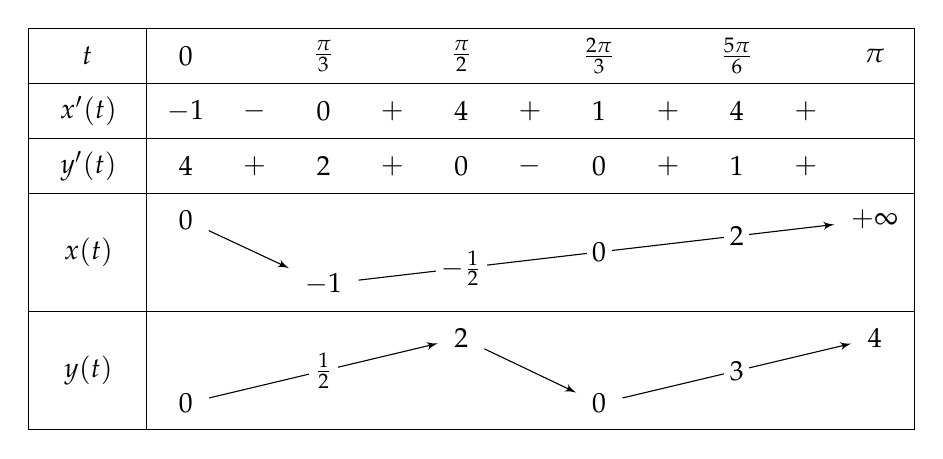
\begin{tikzpicture}
\tkzTabInit[lgt=1.5,espcl=1.75,deltacl=0.5]{$t$/0.7,$x'(t)$/0.7,$y'(t)$/0.7,$x(t)$/1.5,$y(t)$/1.5}{$0$,$\frac\pi3$,$\frac\pi2$,$\frac{2\pi}3$,$\frac{5\pi}6$,$\pi$}
\tkzTabLine{-1,-,0,+,4,+,1,+,4,+,}
\tkzTabLine{4,+,2,+,0,-,0,+,1,+,}
\tkzTabVar{+/$0$,-/$-1$,R/,R/,R/,+/$+\infty$}
\tkzTabIma{2}{6}{3}{$-\frac12$}
\tkzTabIma{2}{6}{4}{$0$}
\tkzTabIma{2}{6}{5}{$2$}
\tkzTabVar{-/$0$,R/,+/$2$,-/$0$,R/,+/$4$}
\tkzTabIma{1}{3}{2}{$\frac12$}
\tkzTabIma{4}{6}{5}{$3$}
\end{tikzpicture}
\end{center}
\begin{enumerate}
\item Dessiner, à partir du tableau, la courbe paramétrée par $f$.
\item Donner l'équation cartésienne de la tangente à la courbe au point de paramètre $t=\frac{5\pi}6$.
\item L'application $g=f_{|]0,\pi]}$ sera-t-elle injective ?
\item Quelle sera l'allure de la courbe entière si, pour $t\in[-\pi,\pi]$, (i) $f$ est impaire ? (ii) $f$ est
      $\pi$-périodique ?
\end{enumerate}
\end{exo}
\begin{exo}{td-c2}{3}{\TD{2}ellipse et échelle}
Une échelle tombe le long d'un mur. On note $\theta\in\left[0,\frac\pi2\right]$ l'angle entre l'échelle et l'horizontale. Soit $M$
un barreau de l'échelle.
\begin{enumerate}
\item Prouver que, dans un repère adapté, la courbe $\mathcal C$ parcourue par $M$ a pour représentation paramétrique
      $x(\theta)=a\cos\theta$, $y(\theta)=b\sin\theta$.
\item En déduire un dessin de $\mathcal C$ point par point en prenant $a=2$ et $b=1$.
\item À quel moment l'échelle est-elle tangente à la courbe $\mathcal C$ ?
\end{enumerate}
\end{exo}

% ---------------------------------------------------------------------
\subsection{Points stationnaires et étude locale}

Au voisinage d'un point, la courbe a l'une des quatre allures du modèle $(t^p,t^q)$, $1\leq p<q$, en $O$ : la corde
$\frac{(t^p,t^q)}{t^p}=(1,t^{q-p})\to(1,0)$ donne la tangente $(Ox)$, et les parités de $p$ et $q$ décident des symétries
(figure~\ref{fig:pq}). \emph{Définition géométrique} : en un \emph{point ordinaire}, la courbe reste du même côté de sa
tangente ; en un \emph{point d'inflexion}, elle la traverse ; en un \emph{point de rebroussement}, elle s'arrête et repart
en arrière, en traversant sa tangente (1\textsuperscript{re} espèce) ou non (2\textsuperscript{e} espèce). Si deux
demi-tangentes existent sans être colinéaires ($f'$ discontinue, comme $(t,|t|)$ en $0$), le point est \emph{anguleux}.

\begin{figure}[H]
\centering
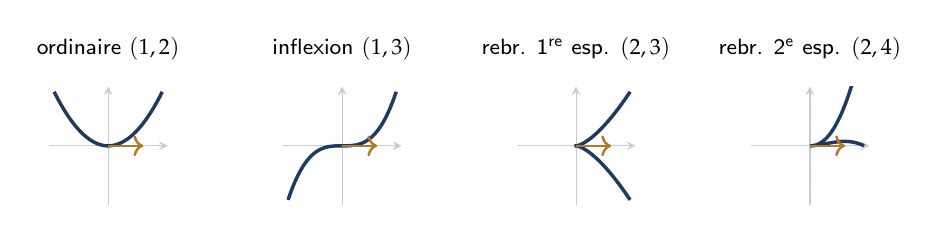
\begin{tikzpicture}
\pgfplotsset{loc/.style={axis lines=middle,axis line style={Filet},width=0.255\linewidth,height=0.255\linewidth,
  xtick=\empty,ytick=\empty,xmin=-1.1,xmax=1.1,ymin=-1.1,ymax=1.1,samples=150,smooth,
  title style={font=\footnotesize\sffamily}}}
\begin{axis}[loc,title={ordinaire $(1,2)$}]
\addplot[arcetude,domain=-1:1]({x},{x^2});\draw[tgte,->](axis cs:0,0)--(axis cs:0.65,0);
\end{axis}
\begin{axis}[loc,xshift=0.245\linewidth,title={inflexion $(1,3)$}]
\addplot[arcetude,domain=-1:1]({x},{x^3});\draw[tgte,->](axis cs:0,0)--(axis cs:0.65,0);
\end{axis}
\begin{axis}[loc,xshift=0.49\linewidth,title={rebr. 1\textsuperscript{re} esp. $(2,3)$}]
\addplot[arcetude,domain=-1:1]({x^2},{x^3});\draw[tgte,->](axis cs:0,0)--(axis cs:0.65,0);
\end{axis}
\begin{axis}[loc,xshift=0.735\linewidth,title={rebr. 2\textsuperscript{e} esp. $(2,4)$}]
\addplot[arcetude,domain=-1:1]({x^2},{x^4+x^5});\draw[tgte,->](axis cs:0,0)--(axis cs:0.65,0);
\end{axis}
\end{tikzpicture}
\caption{Les quatre allures locales (modèles $(t,t^2)$, $(t,t^3)$, $(t^2,t^3)$, $(t^2,t^4+t^5)$) ; la flèche dirige la tangente.}
\label{fig:pq}
\end{figure}

\begin{theoreme}\label{thm:pq}
Soit $f$ de classe $\mathcal C^n$, $p=\min\{k\geq1\mid f^{(k)}(t_0)\neq\ve0\}$ et
$q=\min\{k>p\mid(f^{(p)}(t_0),f^{(k)}(t_0))\text{ libre}\}$ (supposés exister). La tangente est dirigée par $f^{(p)}(t_0)$ et :
\begin{center}
\begin{tabular}{c|cc}
 & $q$ pair & $q$ impair\\\hline
$p$ impair & point ordinaire & inflexion\\
$p$ pair & rebroussement 2\textsuperscript{e} espèce & rebroussement 1\textsuperscript{re} espèce
\end{tabular}
\end{center}
\end{theoreme}

\begin{proof}
Taylor--Young :
\[f(t_0+h)-f(t_0)=f^{(p)}(t_0)\left(\frac{h^p}{p!}+\sum_{k=p+1}^{q-1}\lambda_k\frac{h^k}{k!}\right)+f^{(q)}(t_0)\frac{h^q}{q!}+o(h^q),\]
les dérivées d'ordre $p<k<q$ étant colinéaires à $f^{(p)}(t_0)$. Dans le repère $\big(M(t_0),f^{(p)}(t_0),f^{(q)}(t_0)\big)$,
$X(h)\sim\frac{h^p}{p!}$ et $Y(h)\sim\frac{h^q}{q!}$ : $X$ change de signe avec $h$ si et seulement si $p$ est impair, $Y$ si et
seulement si $q$ est impair, et $Y/X\to0$ donne la tangente.
\end{proof}

\begin{methode}{Étudier un point par développement limité}\label{meth:dl}
Poser $t=t_0+h$ ; développer $x$ et $y$ ; regrouper $f(t_0+h)=f(t_0)+h^p\ve a+\dots+h^q\ve b+o(h^q)$ en s'arrêtant au premier
vecteur $\ve b$ \emph{non colinéaire} à $\ve a$ (tester $\det(\ve a,\ve b)\neq0$). Tangente dirigée par $\ve a$, nature par
$(p,q)$, position : la courbe est du côté de $\ve b$ quand $h^q>0$.
\end{methode}

\begin{exemple}
$f(t)=\big(t-2\sqrt{1+t},\ t\ln(1-t)\big)$ en $0$. Avec $\sqrt{1+t}=1+\frac t2-\frac{t^2}8+\frac{t^3}{16}+o(t^3)$ et
$\ln(1-t)=-t-\frac{t^2}2+o(t^2)$ :
$f(t)=(-2,0)+\frac{t^2}4(1,-4)+\frac{t^3}8(-1,-4)+o(t^3)$, avec $\det\big((1,-4),(-1,-4)\big)=-8\neq0$ : $p=2$, $q=3$,
rebroussement de première espèce en $(-2,0)$, de tangente dirigée par $(1,-4)$.
\end{exemple}

\begin{attention}
Un terme intermédiaire peut être colinéaire au premier (il ne compte pas), ou nul : il faut parfois aller à l'ordre 4 ou 5
(TD~7). Et $f'(t_0)=\ve0$ ne signifie ni « pas de tangente », ni « rebroussement » : $(t^3,t^5)$ a en $0$ une inflexion
($p=3$, $q=5$), $(t^3,t^4)$ un point ordinaire.
\end{attention}

\paragraph{Inflexion et dérivée seconde} Pour un graphe $y=g(x)$, la courbe est au-dessus de ses tangentes là où $g''>0$,
au-dessous là où $g''<0$ ; une inflexion est un point où $g''$ change de signe. On s'y ramène : près d'un point régulier où
$x'(t_0)\neq0$, $y(t)=g\big(x(t)\big)$, et en dérivant deux fois,
\[y'=g'(x)\,x',\qquad y''=g''(x)\,x'^2+g'(x)\,x''\quad\Longrightarrow\quad
g''\big(x(t)\big)=\frac{x'y''-y'x''}{x'^3}=\frac{\det\big(f'(t),f''(t)\big)}{x'(t)^3}.\]

\begin{figure}[H]
\centering
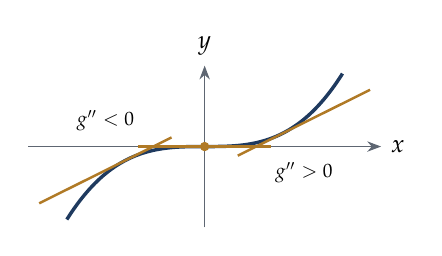
\begin{tikzpicture}
\begin{axis}[courbe,width=0.5\linewidth,height=0.3\linewidth,axis equal image=false,xmin=-1.6,xmax=1.6,ymin=-1.3,ymax=1.3,xtick=\empty,ytick=\empty]
\addplot[arcetude,domain=-1.25:1.25,samples=100]{0.6*x^3};
\addplot[tgte,domain=-1.5:-0.3,samples=2]{0.6*(-0.343)+1.8*0.49*(x+0.7)};
\addplot[tgte,domain=0.3:1.5,samples=2]{0.6*0.343+1.8*0.49*(x-0.7)};
\addplot[tgte,domain=-0.6:0.6,samples=2]{0};
\node[font=\scriptsize,anchor=south] at (axis cs:-0.9,0.1) {$g''<0$};
\node[font=\scriptsize,anchor=north] at (axis cs:0.9,-0.1) {$g''>0$};
\node[pt,fill=Ocre] at (axis cs:0,0) {};
\end{axis}
\end{tikzpicture}
\caption{Le signe de $g''$, donc de $\det(f',f'')$, indique de quel côté de ses tangentes se trouve la courbe (au-dessous
si $g''<0$, au-dessus si $g''>0$) ; à l'inflexion (ocre), il change et la courbe traverse sa tangente.}\label{fig:concavite}
\end{figure}

Comme $x'^3$ garde un signe près de $t_0$ :
\begin{itemize}
\item inflexion $\iff\det(f',f'')$ \emph{change de signe} en $t_0$ ; en particulier $\det(f',f'')=0$ est nécessaire ;
\item si $\det\big(f'(t_0),f''(t_0)\big)\neq0$ (point \emph{birégulier}), $g''\neq0$ : point ordinaire, la courbe étant du côté
      vers lequel pointe $f''(t_0)$ ;
\item la pente $p(t)=g'\big(x(t)\big)=\frac{y'}{x'}$ a pour dérivée $p'=\frac{\det(f',f'')}{x'^2}$ : elle est \emph{extrémale} aux
      inflexions (d'où, en devoir, une racine double pour « la tangente a pour pente $m$ ») ;
\item si $x'(t_0)=0$ (tangente verticale), on échange les rôles : $x=h(y)$ et $h''=-\frac{\det(f',f'')}{y'^3}$. C'est toujours
      $\det(f',f'')$ qui gouverne la concavité (inflexion à tangente verticale : TD~6).
\end{itemize}

\begin{attention}
Ce qui compte est la \emph{colinéarité} de $f''$ et $f'$, pas l'annulation de $f''$ : $(t+t^2,t^3)$ a $f''(0)=(2,0)\neq\ve0$ et une
inflexion en $0$ ($\det=6t(t+1)$ change de signe) ; $(t,t^4)$ a $f''(0)=\ve0$ sans inflexion ($\det=12t^2\geq0$).
\end{attention}

\begin{methode}{Rechercher les points d'inflexion}\label{meth:inflexion}
\begin{enumerate}
\item Candidats : points réguliers où $\det(f',f'')=0$ ; les points stationnaires s'étudient par développement ($p$, $q$ impairs).
\item \emph{Simplifier d'abord} : si $f'=\lambda\ve g$ avec $\lambda$ scalaire non nul, $\det(f',f'')=\lambda^2\det(\ve g,\ve g')$.
      Avec des fonctions trigonométriques, linéariser.
\item Confirmer par le changement de signe (ou par $\det\big(f'(t_0),f'''(t_0)\big)\neq0$, qui donne $q=3$).
\end{enumerate}
\end{methode}

\begin{astuce}
Pour factoriser une somme de cosinus : $e^{ia}\pm e^{ib}=e^{i\frac{a+b}2}\big(e^{i\frac{a-b}2}\pm e^{-i\frac{a-b}2}\big)$, d'où
$\cos t-\cos2t=\mathrm{Re}(e^{it}-e^{2it})=2\sin\frac t2\sin\frac{3t}2$ et $\cos t+\cos2t=2\cos\frac t2\cos\frac{3t}2$.
\end{astuce}

\begin{exo}{td-c4}{4}{\TD{4}cardioïde}
On considère la courbe définie par $x(t)=(1-\cos t)\cos t$, $y(t)=(1-\cos t)\sin t$.
\begin{enumerate}
\item Donner son intervalle d'étude en repérant un axe de symétrie.
\item Prouver que $\cos t-\cos2t=\mathrm{Re}\big(e^{it}-e^{2it}\big)=2\sin\frac t2\sin\frac{3t}2$.
\item Donner le tableau de variation de $x$ et de $y$.
\item Donner la nature du point $O$ et la direction de sa tangente.
\item En déduire l'étude complète de la courbe $\mathcal C$.
\end{enumerate}
\end{exo}
\begin{exo}{td-c6}{3}{\TD{6}points d'inflexion}
On considère la courbe $\mathcal C$ définie pour $t\in\R$ par $x(t)=\frac14(t-2)^3$ et $y(t)=t^2-4$.
\begin{enumerate}
\item Étudier la courbe $\mathcal C$ sur $\R$. $\mathcal C$ admet-elle des asymptotes ?
\item Prouver que $\mathcal C$ possède exactement deux points d'inflexion.
\item Tracer $\mathcal C$ avec ses points d'inflexion.
\end{enumerate}
\end{exo}
\begin{exo}{td-c7}{5}{\TD{7}bicorne, rebroussement de seconde espèce}
Soit $\mathcal B$ représentée par $x(t)=\sin t$, $y(t)=\cos^5t+\frac12\cos^2t$.
\begin{enumerate}
\item Montrer que $M\left(\frac\pi2\right)$ est un point de rebroussement de seconde espèce.
\item Faire l'étude de la courbe en utilisant $\alpha=\arccos\left(\sqrt[3]{-\frac15}\right)$.
\item Dessiner la courbe, sachant qu'au point $A\in\mathcal B$, $A\simeq(0{,}8\,;0{,}1)$, la tangente est horizontale.
\end{enumerate}
\end{exo}

% ---------------------------------------------------------------------
\subsection{Branches infinies}

\begin{definition}
Si $\|\vv{OM(t)}\|\to+\infty$ quand $t\to t_0$, une droite $\mathcal D$ est \emph{asymptote} si $d(M(t),\mathcal D)\to0$.
\end{definition}

\begin{proposition}[distance d'un point à une droite]
Si $\mathcal D:ax+by+c=0$, $d\big(M(x_0,y_0),\mathcal D\big)=\frac{|ax_0+by_0+c|}{\sqrt{a^2+b^2}}$.
\end{proposition}

\begin{proof}
Soient $A\in\mathcal D$, $H$ le projeté de $M$ et $\ve n=(a,b)$, normal à $\mathcal D$ :
$\vv{AM}\cdot\ve n=\vv{HM}\cdot\ve n=\pm HM\,\|\ve n\|$, et $\vv{AM}\cdot\ve n=ax_0+by_0+c$.
\end{proof}

Pour $\mathcal D:y=\alpha x+\beta$, la distance tend vers $0$ si et seulement si $y-\alpha x\to\beta$ ; en divisant par $x$,
$\frac yx\to\alpha$. D'où la méthode.

\begin{methode}{Classer une branche infinie}\label{meth:branches}
Pour chaque borne et chaque valeur interdite $t_0$ :
\begin{enumerate}
\item $x\to\pm\infty$, $y\to b$ : asymptote horizontale $y=b$ ; $x\to a$, $y\to\pm\infty$ : asymptote verticale $x=a$.
\item $x$ et $y$ infinis : $\frac yx\to\pm\infty$ (branche parabolique $(Oy)$), $\to0$ (branche parabolique $(Ox)$), $\to\alpha$ :
      on calcule $\lim(y-\alpha x)$ ; si elle vaut $\beta$, asymptote $y=\alpha x+\beta$ ; si elle est infinie, branche parabolique
      de direction $y=\alpha x$.
\item Position : signe de $y-\alpha x-\beta$, obtenu d'un coup par un \emph{développement asymptotique}.
\item $x$ et $y$ ont des limites finies : \emph{point limite} $A$ ; on le place, et la direction d'arrivée est
      $\lim\frac{y-y_A}{x-x_A}$.
\end{enumerate}
\end{methode}

\begin{methode}{Position globale par rapport à une droite}\label{meth:posglob}
Pour $\mathcal D:ax+by+c=0$, on étudie le signe de $\varphi(t)=ax(t)+by(t)+c$ (fonction numérique) : ses zéros sont les
points d'intersection, son signe le côté. Si $\mathcal D$ est la tangente en $M(t_0)$, $t_0$ est racine au moins double de
$\varphi$, ce qui guide la factorisation de $\varphi'$.
\end{methode}

\begin{horsprogramme}\phantomsection\label{hp:courbe-asymptote}
\textbf{Courbe asymptote.} Une courbe $\Gamma:y=g(x)$ est asymptote si $d(M(t),\Gamma)\to0$ ; on exhibe $P_t\in\Gamma$ avec
$M(t)P_t\to0$ : le point de même abscisse si $y(t)-g(x(t))\to0$ (parabole, cubique), ou de même ordonnée pour une courbe très
pentue (exponentielle). Attention : avec la distance horizontale, si $y=e^x+c$ convient, toutes les constantes $c$
conviennent ($\ln(y-c)-\ln(y-c')\to0$) ; seule la distance verticale en privilégie une.

\textbf{Coordonnées polaires.} $M=O+r(\cos\theta,\sin\theta)$ ; on traduit une équation cartésienne en remplaçant $x$ par
$r\cos\theta$, $y$ par $r\sin\theta$. Cardioïde : $r=1-\cos\theta$ ; lemniscate : $r^2=\frac12\sin2\theta$.
\end{horsprogramme}

\begin{exo}{td-c3}{4}{\TD{3}cissoïde de Dioclès}
Soit $a>0$ et la cissoïde $\mathcal C$ : $x(\theta)=2a\dfrac{\sin^3\theta}{\cos\theta}$, $y(\theta)=2a\sin^2\theta$.
\begin{enumerate}
\item Prouver que $\mathcal C$ possède un axe de symétrie. En déduire un intervalle d'étude.
\item Donner l'équation cartésienne de la tangente $T$ à $\mathcal C$ en $\theta=\frac\pi4$.
\item Donner les tableaux de variation de $x$ et $y$ en fonction de $\theta$.
\item Étudier les points stationnaires de $\mathcal C$.
\item Prouver que la cissoïde possède une asymptote $\mathcal D$ et donner la position de la courbe par rapport à son asymptote.
\item Construction point par point. Soit $A$ le projeté orthogonal de $O$ sur $\mathcal D$. On trace le cercle de diamètre
      $[OA]$ ; pour un point $Q$ du cercle, la droite $(OQ)$ coupe $\mathcal D$ en $H$, et l'on définit $P$ par $\vv{OP}=\vv{QH}$.
      Prouver que l'ensemble de ces points $P$ forme la cissoïde.
\end{enumerate}
\end{exo}
\begin{exo}{td-c5}{4}{\TD{5}lemniscate de Bernoulli}
Soit la courbe $\mathcal L$ parcourue par $M_t$ de coordonnées $x(t)=\dfrac t{1+t^4}$, $y(t)=\dfrac{t^3}{1+t^4}$. Faire l'étude de
$\mathcal L$ et prouver que la droite $y=x$ est axe de symétrie de la courbe. Vérifier que $\mathcal L$ a pour équation en
coordonnées polaires $r^2=\frac{\sin(2\theta)}2$ (\HP).
\end{exo}
\begin{exo}{td-c8}{4}{\TD{8}cubique de Descartes}
On considère la courbe $\mathcal C$ : $x(t)=\dfrac t{1+t^3}$, $y(t)=\dfrac{t^2}{1+t^3}$.
\begin{enumerate}
\item Prouver que $M(t)$ et $M(1/t)$ sont symétriques par rapport à un axe $\Delta$.
\item Faire l'étude de la courbe pour $t\in\,]-1,1[$.
\item Prouver que, pour $t\to-1$, la courbe a pour asymptote $\mathcal D:y=-x-\frac13$ et déterminer la position de la courbe
      par rapport à $\mathcal D$.
\end{enumerate}
\end{exo}
\begin{exo}{td-c9}{5}{\TD{9}axe de symétrie oblique, parabole asymptote \HP}
On considère la courbe $\mathcal C$ définie pour $t\in\R^*$ par $x(t)=t+\dfrac1{2t^2}$ et $y(t)=\dfrac{t^2}2+\dfrac1t$.
\begin{enumerate}
\item Prouver par DL que la courbe présente un point de rebroussement en $M(1)$, et dessiner la courbe au voisinage de
      $M(1)$.
\item Étudier $\mathcal C$ sur $\R^*$.
\item Prouver que $\mathcal C$ admet une parabole asymptote pour $t\to\pm\infty$.
\item Montrer que la droite $y=x$ est axe de symétrie orthogonale de $\mathcal C$. Quel sera le symétrique de $M(t)$ ?
\end{enumerate}
\end{exo}
\begin{exo}{td-c10}{4}{\TD{10}asymptote et prolongement}
On considère la courbe paramétrée $\mathcal C$ par $x(t)=\frac1t$, $y(t)=\frac1{e^t-1}$.
\begin{enumerate}
\item Déterminer l'asymptote $\mathcal D$ à la courbe pour $t\to0$ et indiquer la position de la courbe par rapport à
      l'asymptote.
\item Vérifier que, pour $t\to+\infty$, la courbe $\mathcal C$ se prolonge en un point $A$. Déterminer la tangente à $\mathcal C$
      en ce point $A$.
\item Faire de même pour $t\to-\infty$.
\item En déduire ainsi le tracé de la courbe $\mathcal C$.
\end{enumerate}
\end{exo}

% ---------------------------------------------------------------------
\subsection{Synthèse : une courbe de Lissajous}

\begin{exemple}\label{ex:liss}
$f(t)=(\cos3t,\ 2\sin t)$. Étude, tangentes au point double $J=(0,1)$, autres points communs à la courbe et à l'une de ces
tangentes, points d'inflexion.
\end{exemple}

\q{Réduction.} $f$ est $2\pi$-périodique ; $f(-t)=(x,-y)$ : axe $(Ox)$ ; $f(\pi-t)=(-x,y)$ : axe $(Oy)$. Étude sur
$\left[0,\frac\pi2\right]$ : $x'=-3\sin3t$ (nul en $0$, $\frac\pi3$), $y'=2\cos t>0$ sauf en $\frac\pi2$ : courbe régulière.
$x$ : $1\searrow-1$ ($t=\frac\pi3$) $\nearrow0$ ; $y$ : $0\nearrow2$. Tangentes verticales en $(1,0)$ et $(-1,\sqrt3)$,
horizontale en $(0,2)$.

\q{Point double.} $M\left(\frac\pi6\right)=M\left(\frac{5\pi}6\right)=(0,1)=J$, avec $f'\left(\frac\pi6\right)=(-3,\sqrt3)$ et
$f'\left(\frac{5\pi}6\right)=(-3,-\sqrt3)$ : $T_1:y=-\frac x{\sqrt3}+1$, $T_2:y=\frac x{\sqrt3}+1$.

\q{Intersection de $T_2$ et de la courbe.} $M(t)\in T_2\iff2\sin t=\frac{\cos3t}{\sqrt3}+1$. On pose $X=\cos t$ :
$\cos3t=4X^3-3X$ (partie réelle de $(\cos t+i\sin t)^3$), d'où $2\sqrt3\sin t=4X^3-3X+\sqrt3$. On élève au carré
($\sin^2t=1-X^2$) :
\[P(X)=(4X^3-3X+\sqrt3)^2-12(1-X^2)=16\left(X-\tfrac{\sqrt3}2\right)\left(X+\tfrac{\sqrt3}2\right)^2\left(X^3-\tfrac{\sqrt3}2X^2+\tfrac{\sqrt3}2\right).\]
La racine double $-\frac{\sqrt3}2$ correspond à la tangence ($t=\frac{5\pi}6$), la racine simple $\frac{\sqrt3}2$ au passage de
l'autre branche par $J$ ($t=\frac\pi6$) ; le dernier facteur a une racine réelle $X_0\approx-0{,}735$, pour laquelle
$\sin t=\frac{4X_0^3-3X_0+\sqrt3}{2\sqrt3}\approx0{,}68>0$ (vérification du signe, indispensable après une élévation au
carré). $T_2$ recoupe donc la courbe en un seul autre point, $K\approx(0{,}62\,;1{,}36)$.

\q{Inflexions.} $\det(f',f'')=\dt{-3\sin3t&-9\cos3t\\2\cos t&-2\sin t}=6(\sin3t\sin t+3\cos3t\cos t)$. En posant $u=\tan t$ :
$\tan t\tan3t=-3\iff u^4+6u^2-3=0\iff u^2=2\sqrt3-3$. Plus court : on linéarise,
$\det=12\cos2t+6\cos4t=6(2c^2+2c-1)$ avec $c=\cos2t$, nul pour $c=\frac{\sqrt3-1}2$. Sur $\left[0,\frac\pi2\right]$, une seule
solution $\alpha=\arctan\sqrt{2\sqrt3-3}\approx0{,}598$, où le déterminant change de signe : $M(\alpha)\approx(-0{,}22\,;1{,}13)$
est un point d'inflexion (autre vérification : $\det(f'(\alpha),f'''(\alpha))=-48\sin3\alpha\cos\alpha\neq0$, d'où $q=3$). Par
symétrie, quatre inflexions.

\begin{figure}[H]
\centering
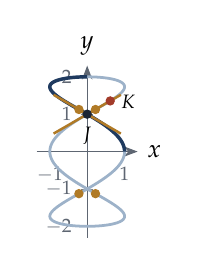
\begin{tikzpicture}
\begin{axis}[courbe,width=0.36\linewidth,xmin=-1.35,xmax=1.35,ymin=-2.3,ymax=2.3,xtick={-1,1},ytick={-2,-1,1,2}]
\addplot[reste,domain=0:6.2832,samples=400]({cos(3*x)},{2*sin(x)});
\addplot[arcetude,domain=0:1.5708,samples=200]({cos(3*x)},{2*sin(x)});
\addplot[tgte,domain=-0.9:0.9,samples=2]{-x/sqrt(3)+1};
\addplot[tgte,domain=-0.9:0.9,samples=2]{x/sqrt(3)+1};
\node[pt] at (axis cs:0,1) {}; \node[font=\scriptsize,anchor=north] at (axis cs:0,0.92) {$J$};
\node[pt,fill=Brique] at (axis cs:0.6154,1.3553) {}; \node[font=\scriptsize,anchor=west] at (axis cs:0.65,1.33) {$K$};
\node[pt,fill=Ocre] at (axis cs:-0.2214,1.126) {}; \node[pt,fill=Ocre] at (axis cs:0.2214,1.126) {};
\node[pt,fill=Ocre] at (axis cs:-0.2214,-1.126) {}; \node[pt,fill=Ocre] at (axis cs:0.2214,-1.126) {};
\end{axis}
\end{tikzpicture}
\caption{La courbe $(\cos3t,2\sin t)$ ; trait plein : arc $\left[0,\frac\pi2\right]$ ; en ocre, les tangentes en $J$ et les
inflexions ; en brique, le point $K$ où $T_2$ recoupe la courbe.}\label{fig:liss}
\end{figure}

% ---------------------------------------------------------------------
\subsection{Fiche : réussir l'étude d'une courbe}

\begin{tcolorbox}[enhanced,breakable,colback=white,colframe=Bleu,boxrule=0.6pt,arc=0pt,left=10pt,right=10pt,top=6pt,bottom=6pt]
\phantomsection\label{fiche:courbe}
\begin{enumerate}[leftmargin=1.4em,itemsep=0.25em]
\item \textbf{Domaine et réduction} : valeurs interdites notées ; chaque symétrie \emph{vérifiée par le calcul}, et compatible
      avec les valeurs connues ($f$ impaire impose $f(0)=O$).
\item \textbf{Dérivées factorisées} (même dénominateur, racines) ; un zéro commun signale un point stationnaire.
\item \textbf{Tangente} : « $x'=0$ donc verticale » seulement si $y'\neq0$ ; en un point stationnaire, développement limité.
\item \textbf{Développement} : jusqu'au premier vecteur non colinéaire au premier ($\det\neq0$), pas plus loin, pas moins.
\item \textbf{Branches} : toutes les bornes et valeurs interdites ; $\lim\frac yx$ ne suffit jamais pour une asymptote ; position par
      développement asymptotique ; limites finies : point limite.
\item \textbf{Position globale} : signe de $\varphi$. \textbf{Inflexions} : factoriser $f'$, puis signe de $\det(f',f'')$.
\item \textbf{Élévation au carré} (intersections) : vérifier les signes à la fin.
\item \textbf{Tracé} : asymptotes, points nommés et tangentes, arcs selon le tableau, positions respectées, symétries.
\end{enumerate}
\end{tcolorbox}

% ---------------------------------------------------------------------
\subsection{Problème type devoir surveillé}

À faire en 1\,h\,30 sans le livre, puis à corriger avec la fiche avant de lire le corrigé.

\begin{exo}{ds-pb}{5}{problème de synthèse, type devoir surveillé}
On considère la courbe $\mathcal C$ définie par
\[x(t)=\frac4t+\ln(3+t),\qquad y(t)=t+\frac4t,\qquad t\in\,]-3,0[\,\cup\,]0,+\infty[,\]
et l'on note $M(t)$ le point de paramètre $t$, $f(t)=\vv{OM(t)}$. Valeurs utiles : $\ln3\approx1{,}10$,
$\ln5\approx1{,}61$, $\ln9\approx2{,}20$, $\ln15\approx2{,}71$.
\begin{enumerate}
\item \textbf{Étude générale et points remarquables.}
\begin{enumerate}
\item Factoriser $x'(t)$ et $y'(t)$, puis dresser le tableau de variations conjoint de $x$ et $y$.
\item Déterminer le point $A$ où la tangente est verticale et le point $B$ où elle est horizontale.
\item Montrer que, en un point régulier, la pente de la tangente vaut $p(t)=\frac{(t-2)(t+3)}{t-6}$. Pour quelles valeurs
      de $m$ existe-t-il un point où la tangente a pour pente $m$ ? Montrer qu'il existe un unique point $H$ où cette pente
      vaut $25$.
\end{enumerate}
\item \textbf{Étude du point $C=M(-2)$.}
\begin{enumerate}
\item En posant $t=-2+h$, écrire le développement limité de $f$ à l'ordre $3$ en $-2$.
\item En déduire la nature du point $C$ et montrer que la tangente $T_C$ a pour équation $x-2y=6$.
\item Préciser la position \emph{locale} de $\mathcal C$ par rapport à $T_C$.
\item En étudiant $\varphi(t)=x(t)-2y(t)-6$, déterminer la position \emph{globale} de $\mathcal C$ par rapport à $T_C$.
\end{enumerate}
\item \textbf{Asymptotes.}
\begin{enumerate}
\item Montrer que $\mathcal C$ admet une asymptote $\Delta_0$ lorsque $t\to0$ et préciser la position.
\item Montrer que $\mathcal C$ admet une autre asymptote $\Delta'$ lorsque $t\to-3$ et préciser la position.
\end{enumerate}
\item \textbf{Branche $t\to+\infty$ (\HP).}
\begin{enumerate}
\item Quelle est la nature de cette branche ?
\item Soit $\mathcal E:y=e^x-7$. En utilisant le point de $\mathcal E$ de même abscisse que $M(t)$, montrer que $\mathcal E$
      est asymptote à $\mathcal C$, et préciser la position.
\item Montrer qu'en utilisant le point de même \emph{ordonnée}, on prouverait de même que toute courbe $y=e^x+c$ est
      asymptote à $\mathcal C$. Commenter.
\end{enumerate}
\item \textbf{Point d'inflexion.}
\begin{enumerate}
\item Écrire $f'(t)=\lambda(t)\,\ve g(t)$ avec $\lambda(t)=\frac{t+2}{t^2(t+3)}$ et $\ve g(t)$ à coordonnées polynomiales,
      puis montrer que $\det\big(f'(t),f''(t)\big)=\lambda(t)^2\det\big(\ve g(t),\ve g'(t)\big)$.
\item En déduire que $\mathcal C$ possède un unique point d'inflexion $N$. Le comparer à $H$ et expliquer.
\item Donner une équation de la tangente $T_N$.
\end{enumerate}
\item \textbf{Dessin.} Tracer $\mathcal C$ en plaçant $A$, $B$, $C$, $N$, les tangentes en ces points et les asymptotes.
\end{enumerate}
\end{exo}

\clearpage
\section{Corrigés}\label{sec:corriges}

Chaque corrigé commence par le \emph{choix de la méthode}, signale les astuces et les pièges, et se termine par ce qu'il faut retenir. On ne le lit qu'après avoir cherché ; s'il a fallu le consulter, on refait l'exercice quelques jours plus tard, sans aide.

\subsection*{Chapitre 1 --- Déterminants}
\addcontentsline{toc}{subsection}{Chapitre 1 --- Déterminants}
\markboth{3\quad Corrigés --- Chapitre 1}{}
\begin{corrige}{td-d8}
\choix{on travaille dans la base $(1,i)$ du $\R$-espace vectoriel $\C$ : on calcule $f(1)$ et $f(i)$, et tout se lit sur la
matrice.}
Posons $a=\alpha+i\beta$. $f$ est $\R$-linéaire ($f(z+\lambda z')=f(z)+\lambda f(z')$). $f(1)=\alpha+i\beta$ et
$f(i)=-\beta+i\alpha$ :
\[\Mat_{(1,i)}(f)=\begin{pmatrix}\alpha&-\beta\\\beta&\alpha\end{pmatrix}.\]
\q{1.} $f\circ g=g\circ f=\Id$ avec $g(z)=\frac za$ ($a\neq0$) : $f$ est bijective et $f^{-1}:z\mapsto a^{-1}z$.

\q{2.} $f$ est une symétrie si et seulement si $f\circ f=\Id$, soit $a^2z=z$ pour tout $z$ : $a^2=1$, $a=\pm1$. Pour $a=1$,
$f=\Id$ (symétrie triviale) ; pour $a=-1$, $f=-\Id$ est la symétrie centrale de centre $O$.

\q{3.} $\mathrm{tr}(f)=2\alpha=2\,\mathrm{Re}(a)$ et $\det(f)=\alpha^2+\beta^2=|a|^2$.

\q{4.} Si $|a|=1$, $a=e^{i\varphi}$ et la matrice est $\begin{pmatrix}\cos\varphi&-\sin\varphi\\\sin\varphi&\cos\varphi\end{pmatrix}$ :
$f$ est la rotation de centre $O$ et d'angle $\varphi=\arg a$.
\gain{le déterminant tranche la question 2 sans calcul : une réflexion (symétrie par rapport à une droite) a pour
déterminant $-1$ (proposition~\ref{prop:proj-sym}, $\dim\mathrm{Ker}(s+\Id)=1$), alors que $\det f=|a|^2>0$. Une similitude
$z\mapsto az$ n'est donc jamais une réflexion ; c'est $z\mapsto a\overline z$ ($|a|=1$) qui en donne, avec
$\det=-|a|^2$.}
\piege{$\C$ est ici un $\R$-espace vectoriel de dimension $2$ : la trace et le déterminant se calculent sur une matrice
$2\times2$ réelle, pas sur le « scalaire » $a$.}
\retenir{$\det f>0$ : $f$ conserve l'orientation (rotations, similitudes directes) ; $\det f<0$ : elle la renverse (réflexions).
Le module $|a|$ est le rapport de dilatation des longueurs, $|a|^2=\det f$ celui des aires.}
\end{corrige}
\begin{corrige}{g-carre}
\choix{on ne connaît aucun coefficient, seulement une relation : on prend le déterminant des deux membres.}
$\det(A)^2=\det(A^2)=\det(-I_n)=(-1)^n$. Comme $\det A$ est réel, $\det(A)^2\geq0$, donc $(-1)^n>0$ (il ne peut valoir $0$) : $n$
est pair. Pour une matrice complexe, $A=iI_n$ convient pour tout $n$ : le résultat tombe, car $\det(A)^2$ peut être négatif.
\retenir{relation entre matrices $\Rightarrow$ appliquer $\det$ ($\det(AB)$, $\det(\lambda A)=\lambda^n\det A$). Exemple voisin : une
matrice antisymétrique réelle d'ordre impair n'est pas inversible ($\det A=\det A^T=\det(-A)=-\det A$).}
\end{corrige}
\begin{corrige}{b-endo}
\choix{choisir l'ordre des vecteurs de base pour obtenir une matrice diagonale par blocs : $(E_{1,1},E_{2,1},E_{1,2},E_{2,2})$,
c'est-à-dire colonne par colonne, car $AM$ agit sur chaque colonne de $M$.}
$AE_{1,1}=aE_{1,1}+cE_{2,1}$, $AE_{2,1}=bE_{1,1}+dE_{2,1}$, et de même pour la seconde colonne. Dans cette base,
$\Mat(f)=\begin{pmatrix}A&0\\0&A\end{pmatrix}$ ; en développant (ou par le déterminant diagonal par blocs),
$\det f=(\det A)^2$. Donc $f$ est bijectif si et seulement si $A$ est inversible, et alors $f^{-1}(M)=A^{-1}M$.
\piege{dans l'ordre usuel $(E_{1,1},E_{1,2},E_{2,1},E_{2,2})$, la matrice n'est pas diagonale par blocs : le résultat est le
même, mais le calcul est plus long. Le choix de la base fait la moitié du travail.}
\retenir{en dimension $n$, $\det(M\mapsto AM)=(\det A)^n$ (une copie de $A$ par colonne).}
\end{corrige}
\begin{corrige}{hp-com}
\choix{on applique la formule de la comatrice (encadré du \S1.3) ; les questions 2 et 3 reposent sur
$A\,\mathrm{com}(A)^T=\det(A)I_n$.}
\q{1.} $\det A=1\cdot1-2\cdot(0-1)=3$. Les cofacteurs, ligne par ligne :
$\mathrm{com}(A)=\begin{pmatrix}1&1&-1\\-2&1&2\\2&-1&1\end{pmatrix}$, d'où
$A^{-1}=\frac13\mathrm{com}(A)^T=\frac13\begin{pmatrix}1&-2&2\\1&1&-1\\-1&2&1\end{pmatrix}$. On vérifie $AA^{-1}=I_3$.

\q{2.} Si $\det A=\pm1$, $A^{-1}=\pm\mathrm{com}(A)^T$ est entière (cofacteurs entiers). Réciproquement, $\det A$ et $\det A^{-1}$
sont des entiers de produit $1$.

\q{3.} $\det A\cdot\det\mathrm{com}(A)=\det(\det(A)I_n)=(\det A)^n$, d'où $\det\mathrm{com}(A)=(\det A)^{n-1}$.
\piege{la comatrice se \emph{transpose} avant de diviser par $\det A$ ; et chaque cofacteur porte son signe $(-1)^{i+j}$.}
\retenir{$A^{-1}=\frac1{\det A}\mathrm{com}(A)^T$ ; en taille 2 : échanger la diagonale, changer les signes du reste.}
\end{corrige}
\begin{corrige}{td-d1}
\choix{l'alignement se traduit par $\det(\vv{AB},\vv{AC})=0$. Il faut donc faire apparaître les coordonnées de $\vv{AB}$
et $\vv{AC}$, c'est-à-dire des \emph{différences} $b-a$, $c-a$ : ce sont des transvections de colonnes.}
$C_2\leftarrow C_2-C_1$ et $C_3\leftarrow C_3-C_1$ ne changent pas le déterminant :
\[\dt{1&1&1\\a&b&c\\a'&b'&c'}=\dt{1&0&0\\a&b-a&c-a\\a'&b'-a'&c'-a'}=\dt{b-a&c-a\\b'-a'&c'-a'}=\det(\vv{AB},\vv{AC}),\]
en développant selon la première ligne. Le déterminant est nul si et seulement si $\vv{AB}$ et $\vv{AC}$ sont colinéaires,
c'est-à-dire si $A$, $B$, $C$ sont alignés. On a donc l'équivalence, pas seulement l'implication demandée.
\gain{la ligne de $1$ « absorbe » le point $A$ : retrancher la première colonne transforme des points en vecteurs. En
remplaçant $C$ par un point courant $M(x,y)$, on obtient sans calcul l'équation de la droite $(AB)$ :
$\dt{1&1&1\\a&b&x\\a'&b'&y}=0$.}
\retenir{trois points $A$, $B$, $M$ du plan sont alignés si et seulement si le déterminant de la matrice dont les colonnes sont
$(1,x,y)$ pour chacun d'eux est nul. En dimension 3, même chose avec quatre points et une ligne de $1$ : coplanarité.}
\end{corrige}
\begin{corrige}{td-d2}
\choix{la distance de deux droites est la plus petite distance $MN$, $M\in(AB)$, $N\in(CD)$. On cherche le couple $(H,K)$
qui la réalise (perpendiculaire commune), puis on reconnaît dans le produit mixte un volume « base fois hauteur ».}
Notons $\ve u=\vv{AB}$, $\ve v=\vv{CD}$, $\ve n=\ve u\wedge\ve v\neq\ve0$ (droites non parallèles).

\q{1. Existence de la perpendiculaire commune.} On cherche $H=A+s\ve u$ et $K=C+r\ve v$ avec $\vv{HK}\cdot\ve u=0$ et
$\vv{HK}\cdot\ve v=0$. Comme $\vv{HK}=\vv{AC}+r\ve v-s\ve u$, c'est le système
\[s\|\ve u\|^2-r\,\ve u\cdot\ve v=\vv{AC}\cdot\ve u,\qquad s\,\ve u\cdot\ve v-r\|\ve v\|^2=\vv{AC}\cdot\ve v,\]
de déterminant $-\|\ve u\|^2\|\ve v\|^2+(\ve u\cdot\ve v)^2=-\|\ve u\wedge\ve v\|^2\neq0$ : il a une unique solution.

\q{2. $HK$ est la distance.} Pour $M\in(AB)$, $N\in(CD)$ : $\vv{MN}=\vv{HK}+(\vv{MH}+\vv{KN})$ avec
$\vv{MH}+\vv{KN}\in\vect(\ve u,\ve v)$, orthogonal à $\vv{HK}$. Par Pythagore, $MN^2=HK^2+\|\vv{MH}+\vv{KN}\|^2\geq HK^2$.

\q{3. La formule.} Par permutation circulaire, $\det(\ve u,\ve v,\vv{AC})=(\ve u\wedge\ve v)\cdot\vv{AC}$. On décompose
$\vv{AC}=\vv{AH}+\vv{HK}+\vv{KC}$ : $\vv{AH}\in\vect(\ve u)$ et $\vv{KC}\in\vect(\ve v)$ sont orthogonaux à $\ve n$, d'où
$\ve n\cdot\vv{AC}=\ve n\cdot\vv{HK}$. Comme $\vv{HK}$ est orthogonal à $\ve u$ et $\ve v$, il est colinéaire à $\ve n$ :
$|\ve n\cdot\vv{HK}|=\|\ve n\|\,HK$. Donc $HK=\frac{|\det(\ve u,\ve v,\vv{AC})|}{\|\ve u\wedge\ve v\|}$.
\gain{interprétation éclair (figure~\ref{fig:dist-droites}) : $|\det(\ve u,\ve v,\vv{AC})|$ est le volume du parallélépipède
de base $\|\ve u\wedge\ve v\|$ ; la hauteur est la distance cherchée. Retrouver la formule par « volume / base » évite de
l'apprendre.}
\piege{le point de $\vv{AC}$ est arbitraire : on peut prendre n'importe quel point de chaque droite ($\vv{AD}$, $\vv{BC}$\dots),
le résultat ne change pas. Si les droites sont parallèles, $\ve u\wedge\ve v=\ve0$ et la formule n'a pas de sens : on calcule
alors la distance d'un point de l'une à l'autre.}
\retenir{droites sécantes $\iff$ coplanaires et non parallèles $\iff\det(\vv{AC},\ve u,\ve v)=0$ avec $\ve u\wedge\ve v\neq\ve0$.
Technique réutilisable : décomposer un vecteur selon une base adaptée, puis projeter sur la normale.}
\end{corrige}
\begin{corrige}{td-d6}
\choix{« $n$ vecteurs en dimension $n$, base ? » : on calcule $\det_{\mathcal B}(\mathcal C)$ (théorème~\ref{thm:base}). La
matrice a la même somme sur chaque ligne : proposition~\ref{prop:ab}.}
La matrice de $\mathcal C$ dans $\mathcal B$ a des $a$ sur la diagonale et des $b$ ailleurs. Chaque ligne a pour somme
$a+(n-1)b$ ; $C_1\leftarrow C_1+\dots+C_n$, on sort ce facteur, puis $L_i\leftarrow L_i-L_1$ :
\[\det_{\mathcal B}(\mathcal C)=\big(a+(n-1)b\big)\dt{1&b&\cdots&b\\0&a-b&&(0)\\\vdots&&\ddots&\\0&(0)&&a-b}=\big(a+(n-1)b\big)(a-b)^{n-1}.\]
$\mathcal C$ est une base si et seulement si ce produit est non nul, c'est-à-dire $a+(n-1)b\neq0$ et $a\neq b$ (pour $n\geq2$).
\piege{pour $n=1$, $\delta_1=ae_1$ et la condition est seulement $a\neq0$ : le facteur $(a-b)^{n-1}=1$ disparaît. L'énoncé
suppose implicitement $n\geq2$.}
\gain{la matrice s'écrit $(a-b)I_n+bJ$ ($J$ : que des $1$). Cette écriture donne aussi l'inverse et les valeurs propres ; elle
revient souvent.}
\retenir{$D_n(a,b)=(a+(n-1)b)(a-b)^{n-1}$ est à connaître ; la méthode « somme constante » s'applique dès que les lignes (ou
les colonnes) ont même somme.}
\end{corrige}
\begin{corrige}{f-absij}
\choix{comme pour $\max(i,j)$ (exemple~\ref{ex:max}) : différences de colonnes, puis une seconde vague sur les lignes.}
\q{Colonnes.} Pour $k$ de $n$ à $2$, $C_k\leftarrow C_k-C_{k-1}$ : le coefficient $(i,k)$ devient $|i-k|-|i-k+1|$, soit $1$ si
$i<k$ et $-1$ si $i\geq k$. La première colonne reste $(0,1,\dots,n-1)^T$.

\q{Lignes.} Pour $i$ de $n$ à $2$, $L_i\leftarrow L_i-L_{i-1}$ : la ligne $i$ devient $(1,0,\dots,0,-2,0,\dots,0)$, le $-2$ en
colonne $i$ ; la ligne $1$ reste $(0,1,\dots,1)$.

\q{Conclure.} $C_1\leftarrow C_1+\frac12(C_2+\dots+C_n)$ annule la première colonne sauf son premier coefficient,
$\frac{n-1}2$. Matrice triangulaire de diagonale $\left(\frac{n-1}2,-2,\dots,-2\right)$ :
\[B_n=\frac{n-1}2(-2)^{n-1}=(-1)^{n-1}(n-1)2^{n-2}.\]
Contrôle : $B_2=-1$, $B_3=4$.
\gain{dans la 3\textsuperscript{e} étape, on combine les colonnes pour annuler les $1$ de la première colonne : chaque $-2$
« absorbe » un $1$ avec le coefficient $\frac12$.}
\retenir{différences de colonnes, puis de lignes : chaque vague simplifie d'un cran. Toujours dans l'ordre $k=n,n-1,\dots,2$.}
\end{corrige}
\begin{corrige}{f-ka}
\choix{au-dessus de la diagonale, la colonne $k$ vaut $a$ fois la colonne $k-1$ : on retranche $aC_{k-1}$ (et non $C_{k-1}$).}
Pour $k$ de $n$ à $2$, $C_k\leftarrow C_k-aC_{k-1}$ : pour $i<k$, $a^{k-i}-a\cdot a^{k-1-i}=0$ ; pour $i\geq k$,
$a^{i-k}-a\cdot a^{i-k+1}=a^{i-k}(1-a^2)$. Matrice triangulaire inférieure de diagonale $(1,1-a^2,\dots,1-a^2)$ :
$\det=(1-a^2)^{n-1}$.
\retenir{adapter le coefficient de la différence à la structure ; contrôle immédiat : pour $a=\pm1$, les colonnes sont égales ou
opposées, le déterminant est nul.}
\end{corrige}
\begin{corrige}{td-d4}
\choix{la première et la dernière ligne n'ont que deux coefficients non nuls, et en les supprimant on retrouve un X plus
petit : récurrence. Seconde méthode, plus rapide : regrouper les coefficients non nuls en blocs.}
\q{Méthode 1 : récurrence.} Notons $D_{2n}$ ce déterminant. En développant selon la première ligne $(a,0,\dots,0,b)$ :
$D_{2n}=a\,\Delta_{1,1}+(-1)^{1+2n}b\,\Delta_{1,2n}=a\Delta_{1,1}-b\Delta_{1,2n}$.
\begin{itemize}
\item Dans $\Delta_{1,1}$, la dernière ligne est $(0,\dots,0,a)$ ; on développe selon elle : $\Delta_{1,1}=a\,D_{2n-2}$ (le
      bloc central est le X d'ordre $2n-2$).
\item Dans $\Delta_{1,2n}$, la dernière ligne est $(b,0,\dots,0)$, en position $(2n-1,1)$, de signe $(-1)^{2n}=+1$ :
      $\Delta_{1,2n}=b\,D_{2n-2}$.
\end{itemize}
D'où $D_{2n}=(a^2-b^2)D_{2n-2}$, avec $D_2=a^2-b^2$ : $\boxed{D_{2n}=(a^2-b^2)^n}$.

\q{Méthode 2 : permutation.} On réordonne lignes \emph{et} colonnes selon $1,2n,2,2n-1,\dots,n,n+1$ ; le déterminant ne change
pas. La matrice devient diagonale par blocs, de $n$ blocs $\begin{pmatrix}a&b\\b&a\end{pmatrix}$ : $(a^2-b^2)^n$ en une ligne.
\piege{les signes du développement : le coefficient $b$ de la première ligne est en position $(1,2n)$, de signe $(-1)^{2n+1}=-1$.
Une erreur de signe donnerait $(a^2+b^2)^n$, faux dès $n=1$.}
\gain{en taille impaire $2n+1$, le coefficient central est seul sur sa ligne : on développe selon lui et l'on se ramène au cas
pair, d'où $a(a^2-b^2)^n$.}
\retenir{deux idées réutilisables : un développement qui reproduit la forme initiale donne une récurrence ; une même
permutation des lignes et des colonnes conserve le déterminant et révèle des blocs.}
\end{corrige}
\begin{corrige}{td-d9}
\choix{les lignes $2$ à $n-1$ n'ont qu'un coefficient : on les « sort », puis on s'en sert comme pivots pour nettoyer les lignes
$1$ et $n$.}
\q{Factoriser.} On sort $b_{n+1-k}$ de chaque ligne $k$ ($2\leq k\leq n-1$) : facteur $b_2b_3\cdots b_{n-1}$ ; la ligne $k$ devient le
vecteur ligne $e_{n+1-k}$ (un $1$ en colonne $n+1-k$).

\q{Nettoyer.} Pour chaque colonne $j\in\ient2{n-1}$, on retranche à la ligne $1$ (resp. $n$) $a_j$ (resp. $c_j$) fois la ligne
ayant un $1$ en colonne $j$ (transvections) : les lignes $1$ et $n$ deviennent $(a_1,0,\dots,0,a_n)$ et $(c_1,0,\dots,0,c_n)$.

\q{Remettre dans l'ordre.} Les lignes $2$ à $n-1$ forment une « anti-identité » sur les colonnes $2$ à $n-1$. Inverser l'ordre
de ces $n-2$ lignes demande $\left\lfloor\frac{n-2}2\right\rfloor$ échanges. On obtient alors une identité au centre ; en
développant selon les lignes $2,\dots,n-1$ (un seul $1$, en position diagonale, signe $+$), il reste
$\dt{a_1&a_n\\c_1&c_n}$. Donc
\[\det D=(-1)^{\lfloor\frac{n-2}2\rfloor}\,b_2b_3\cdots b_{n-1}\,(a_1c_n-a_nc_1).\]
Contrôle : $n=3$, $D=\dt{a_1&a_2&a_3\\0&b_2&0\\c_1&c_2&c_3}=b_2(a_1c_3-a_3c_1)$, en développant selon la ligne 2.
\gain{le nombre d'échanges pour inverser $m$ objets est $\lfloor m/2\rfloor$ (on échange le premier et le dernier, etc.) ; la
parité de $\lfloor m/2\rfloor$ est celle de $\frac{m(m-1)}2$.}
\piege{oublier le signe de l'anti-diagonale. Le déterminant « en N » (les $b_j$ sur la diagonale au lieu de l'anti-diagonale)
n'a pas ce signe : $b_2\cdots b_{n-1}(a_1c_n-a_nc_1)$.}
\retenir{face à une ligne n'ayant qu'un coefficient : la sortir comme facteur, puis l'utiliser comme pivot. Toujours tester la
formule finale sur $n=3$ ou $4$.}
\end{corrige}
\begin{corrige}{td-d5}
\choix{$x$ n'apparaît que dans la dernière colonne : méthode~\ref{meth:poly}. On ne développe surtout pas « à la main » : on
utilise la structure (degré, coefficient dominant, racines).}
\q{1.} En développant selon la dernière colonne $(1,x,x^2,x^3)^T$,
$P(x)=\gamma_0+\gamma_1x+\gamma_2x^2+\gamma_3x^3$, où les $\gamma_k$ sont des cofacteurs indépendants de $x$ : $P$ est un
polynôme de degré au plus $3$. Son coefficient de $x^3$ est le cofacteur $(-1)^{4+4}\Delta_{4,4}$,
\[\gamma_3=\dt{1&1&1\\a&b&c\\a^2&b^2&c^2}=(b-a)(c-a)(c-b)\]
(Vandermonde d'ordre 3 : $C_2\leftarrow C_2-C_1$, $C_3\leftarrow C_3-C_1$, puis on sort $b-a$ et $c-a$). Enfin $P(a)=P(b)=P(c)=0$
(deux colonnes égales).
\begin{itemize}
\item Si $a,b,c$ sont distincts, $\gamma_3\neq0$ : $P$ est de degré $3$ et ses racines sont exactement $a$, $b$, $c$.
\item Sinon, $A$ a deux colonnes égales pour tout $x$ : $P=0$.
\end{itemize}
\q{2.} Un polynôme de degré $3$ de coefficient dominant $\gamma_3$ et de racines $a,b,c$ vaut $\gamma_3(x-a)(x-b)(x-c)$ :
\[\det A=(b-a)(c-a)(c-b)(x-a)(x-b)(x-c),\]
formule vraie aussi lorsque $a,b,c$ ne sont pas distincts (les deux membres sont nuls).

\q{3.} Notons $V_n(a_1,\dots,a_n)$ ce déterminant. La propriété est vraie pour $n=2$ : $V_2=a_2-a_1$. Supposons-la vraie au rang
$n-1$. Remplaçons $a_n$ par $x$ : comme en 1, $Q(x)=V_n(a_1,\dots,a_{n-1},x)$ est un polynôme de degré au plus $n-1$, de
coefficient de $x^{n-1}$ égal au cofacteur $V_{n-1}(a_1,\dots,a_{n-1})$, et s'annule en $a_1,\dots,a_{n-1}$. Si les $a_p$
($p<n$) sont distincts, $Q(x)=V_{n-1}(a_1,\dots,a_{n-1})\prod_{p=1}^{n-1}(x-a_p)$ ; sinon les deux membres sont nuls. En
$x=a_n$ et par hypothèse de récurrence :
\[V_n=\prod_{k=2}^{n-1}\prod_{p=1}^{k-1}(a_k-a_p)\times\prod_{p=1}^{n-1}(a_n-a_p)=\prod_{k=2}^n\prod_{p=1}^{k-1}(a_k-a_p).\]
\gain{le coefficient dominant se lit sans calcul : c'est le mineur qui reste quand on barre la ligne et la colonne de
$x^{n-1}$. Et les racines évidentes viennent de « deux colonnes égales ».}
\piege{oublier le cas où les $a_p$ ne sont pas distincts (le degré chute) ; il se règle en une phrase, mais il faut l'écrire.}
\retenir{la méthode du polynôme s'applique dès qu'une variable n'occupe qu'une ligne ou une colonne. $V\neq0\iff$ les points
sont distincts : c'est l'outil de l'interpolation de Lagrange et de la liberté des familles $(x\mapsto e^{\alpha_ix})$.}
\end{corrige}
\begin{corrige}{td-d3}
\choix{commencer par \emph{dessiner} la matrice : les symboles de Kronecker cachent un tridiagonal. Puis méthode~\ref{meth:rec}.}
$\delta_{i,j-1}=1$ si et seulement si $j=i+1$ : des $6$ juste au-dessus de la diagonale ; $\delta_{i-1,j}=1$ si et seulement si
$i=j+1$ : des $1$ juste au-dessous ; des $5$ sur la diagonale.
\[A_4=\begin{pmatrix}5&6&0&0\\1&5&6&0\\0&1&5&6\\0&0&1&5\end{pmatrix}.\]
\q{Récurrence.} On développe $u_n$ selon la première ligne $(5,6,0,\dots,0)$ :
$u_n=5u_{n-1}-6\Delta_{1,2}$. Le mineur $\Delta_{1,2}$ a pour première colonne $(1,0,\dots,0)^T$ ; en le développant selon
elle, $\Delta_{1,2}=1\cdot u_{n-2}$. Donc
\[u_n=5u_{n-1}-6u_{n-2}\quad(n\geq3),\qquad u_1=5,\ u_2=25-6=19.\]
\q{1.} $u_3=5\cdot19-6\cdot5=65$, puis $\det(A_4)=u_4=5\cdot65-6\cdot19=211$.

\q{2.} L'équation caractéristique $r^2-5r+6=0$ a pour racines $2$ et $3$ : $u_n=\alpha2^n+\beta3^n$. Avec
$2\alpha+3\beta=5$ et $4\alpha+9\beta=19$ : $\beta=3$, $\alpha=-2$, d'où
\[u_n=3^{n+1}-2^{n+1}.\]
Contrôle : $u_4=243-32=211$.
\gain{on peut poser $u_0=1$ (valeur qui rend la relation vraie pour $n=2$ : $19=5\cdot5-6u_0$) : les conditions $u_0=1$, $u_1=5$
donnent les constantes plus vite. Et seul le produit $6\times1$ des coefficients hors diagonale compte : échanger $6$ et $1$ ne
change rien.}
\piege{oublier le signe $(-1)^{1+2}=-1$ du coefficient $6$, ce qui donne $u_n=5u_{n-1}+6u_{n-2}$ ; le contrôle sur $u_3$ (calculé
par Sarrus) détecte l'erreur.}
\retenir{tridiagonal (diagonale $a$, voisins $b$ et $c$) $\Rightarrow T_n=aT_{n-1}-bc\,T_{n-2}$ ; toujours vérifier la formule
finale sur un petit $n$.}
\end{corrige}
\begin{corrige}{td-d7}
\choix{tridiagonal : récurrence (méthode~\ref{meth:rec}). Comme le résultat est donné, la vérification par récurrence avec une
formule de trigonométrie est plus courte que la résolution.}
Notons $D_n=\det(A_n)$. Le développement donne $D_n=2\cos\theta\,D_{n-1}-D_{n-2}$ ($bc=1$), avec $D_1=2\cos\theta$ et
$D_2=4\cos^2\theta-1$. On suppose $\theta\notin\pi\Z$.
\begin{itemize}
\item $\frac{\sin2\theta}{\sin\theta}=2\cos\theta=D_1$ et $\frac{\sin3\theta}{\sin\theta}=4\cos^2\theta-1=D_2$, car
      $\sin3\theta=3\sin\theta-4\sin^3\theta=\sin\theta(4\cos^2\theta-1)$.
\item Si la formule est vraie aux rangs $n-1$ et $n-2$, la formule
      $\sin\big((n+1)\theta\big)+\sin\big((n-1)\theta\big)=2\sin(n\theta)\cos\theta$ donne
      $2\cos\theta D_{n-1}-D_{n-2}=\frac{\sin((n+1)\theta)}{\sin\theta}$ : elle est vraie au rang $n$.
\end{itemize}
Si $\theta\in\pi\Z$, $\cos\theta=\varepsilon=\pm1$ : racine double $\varepsilon$, et $D_n=(n+1)\varepsilon^n$, qui est la
limite de $\frac{\sin((n+1)\theta)}{\sin\theta}$.
\gain{pour \emph{trouver} la formule sans la connaître : $r^2-2\cos\theta\,r+1=0$ a pour racines $e^{\pm i\theta}$, donc
$D_n=\lambda\cos n\theta+\mu\sin n\theta$ ; avec $D_0=1$ et $D_1=2\cos\theta$, on obtient $\lambda=1$,
$\mu=\frac{\cos\theta}{\sin\theta}$, et $D_n=\frac{\sin\theta\cos n\theta+\cos\theta\sin n\theta}{\sin\theta}$.}
\piege{la formule n'a pas de sens pour $\theta\in\pi\Z$ : il faut traiter ce cas à part (racine double).}
\retenir{prolongement classique : $D_n=0\iff\theta=\frac{k\pi}{n+1}$ ($1\leq k\leq n$). Le déterminant d'ordre $n$ à diagonale $x$
et voisins $1$ est un polynôme unitaire de degré $n$ ; il a ces $n$ racines distinctes $2\cos\frac{k\pi}{n+1}$, donc n'en a pas
d'autre.}
\end{corrige}
\begin{corrige}{td-d10}
\choix{retrancher $x$ partout transforme les coefficients constants $a$ et $b$ en $a-x$ et $b-x$ : pour $x=a$ ou $x=b$, la
matrice devient triangulaire. Il suffit donc de savoir que $P$ est affine (méthode~\ref{meth:affine}).}
Notons $Q(x)=\prod_{i=1}^n(\lambda_i-x)$.

\q{1.} Les colonnes de $A_n-xU$ sont $C_j-xU_1$, où $U_1=(1,\dots,1)^T$. Les transvections $C_j\leftarrow C_j-C_1$ ($j\geq2$)
donnent des colonnes $C_j-C_1$ indépendantes de $x$ ; seule la première, $C_1-xU_1$, dépend de $x$. Par linéarité selon la
première colonne :
\[P(x)=\det(C_1,C_2-C_1,\dots)-x\det(U_1,C_2-C_1,\dots)=\beta-\alpha x :\quad\deg P\leq1.\]
\q{2.} $A_n-aU$ a des $0$ au-dessus de la diagonale : triangulaire inférieure, $P(a)=\prod(\lambda_i-a)=Q(a)$. De même
$P(b)=Q(b)$. Comme $\det A_n=P(0)$ et que $P$ est affine, on écrit la droite passant par $(a,Q(a))$ et $(b,Q(b))$ :
\[\det A_n=P(0)=\frac{b\,Q(a)-a\,Q(b)}{b-a}\qquad(a\neq b).\]
(Vérification : en $x=a$, la droite $x\mapsto\frac{(b-x)Q(a)-(a-x)Q(b)}{b-a}$ vaut bien $Q(a)$.)

\q{3.} Pour $a$ fixé, $b\mapsto\det A_n$ est polynomiale, donc continue : on fait tendre $b$ vers $a$. Avec
$\varphi(u)=u\,Q(a)-a\,Q(u)$, on a $\varphi(a)=0$ et $\det A_n=\frac{\varphi(b)-\varphi(a)}{b-a}\to\varphi'(a)$. D'où, pour $a=b$,
\[\det A_n=Q(a)-aQ'(a)=\prod_{i=1}^n(\lambda_i-a)+a\sum_{j=1}^n\prod_{i\neq j}(\lambda_i-a).\]
Contrôle : tous les $\lambda_i$ égaux à $\lambda$ : $(\lambda-a)^n+na(\lambda-a)^{n-1}=(\lambda+(n-1)a)(\lambda-a)^{n-1}$, c'est la
proposition~\ref{prop:ab}.
\gain{reconnaître un \emph{taux d'accroissement} : une expression $\frac{\varphi(b)-\varphi(a)}{b-a}$ avec $\varphi(a)=0$ tend vers
$\varphi'(a)$. C'est le sens de « à l'aide d'une dérivée ».}
\piege{en 3, on ne peut pas faire $b=a$ dans la formule de la question 2 (division par $0$) ; il faut justifier le passage à la
limite par la continuité du déterminant.}
\retenir{trois techniques : (i) $x$ ajouté partout $\Rightarrow$ affine ; (ii) choisir les valeurs de $x$ qui rendent la matrice
triangulaire ; (iii) prolonger une formule par continuité, la limite étant une dérivée.}
\end{corrige}
\begin{corrige}{det-pb}
\choix{coefficients constants au-dessus et au-dessous : c'est la situation du TD~10, que l'on applique avec $\lambda_i=x$,
$a=1$, $b=-1$.}
\q{1.} Avec $D(c)$ le déterminant obtenu en ajoutant $c$ partout (affine) : $D(-1)=(x-1)^n$ (triangulaire inférieure),
$D(1)=(x+1)^n$ (triangulaire supérieure), et pour une fonction affine $D(0)=\frac{D(1)+D(-1)}2$.

\q{2.} $n$ pair : somme de deux puissances paires qui ne s'annulent pas ensemble, $\det>0$ : toujours inversible. $n$ impair :
$(x+1)^n=(1-x)^n\iff x+1=1-x\iff x=0$ (injectivité de $u\mapsto u^n$) : inversible si et seulement si $x\neq0$.
\retenir{pour $x=0$, $M_n(0)$ est antisymétrique : on retrouve qu'en ordre impair son déterminant est nul.}
\end{corrige}

\subsection*{Chapitre 2 --- Courbes paramétrées}
\addcontentsline{toc}{subsection}{Chapitre 2 --- Courbes paramétrées}
\markboth{3\quad Corrigés --- Chapitre 2}{}
\begin{corrige}{td-c1}
\choix{chaque colonne du tableau est un point avec sa tangente (donnée par $(x',y')$), chaque intervalle un arc dont la
direction est donnée par les signes de $(x',y')$. Pour l'injectivité, on raisonne sur les \emph{arcs} où $x$ est monotone.}
\q{1. Points et tangentes.}
\begin{itemize}
\item $t=0$ : $O$, $f'=(-1,4)$, tangente de pente $-4$ ;
\item $t=\frac\pi3$ : $\left(-1,\frac12\right)$, $f'=(0,2)$ : tangente verticale ;
\item $t=\frac\pi2$ : $\left(-\frac12,2\right)$, $f'=(4,0)$ : tangente horizontale ;
\item $t=\frac{2\pi}3$ : $O$ à nouveau, $f'=(1,0)$ : tangente horizontale ;
\item $t=\frac{5\pi}6$ : $(2,3)$, $f'=(4,1)$ ;
\item $t\to\pi$ : $x\to+\infty$, $y\to4$ : asymptote horizontale $y=4$, la courbe est au-dessous ($y$ croît vers $4$).
\end{itemize}
Arcs : vers le haut à gauche sur $\left[0,\frac\pi3\right]$, vers le haut à droite jusqu'à $\frac\pi2$, vers le bas à droite
jusqu'à $\frac{2\pi}3$ (retour en $O$), puis vers le haut à droite.
\begin{center}
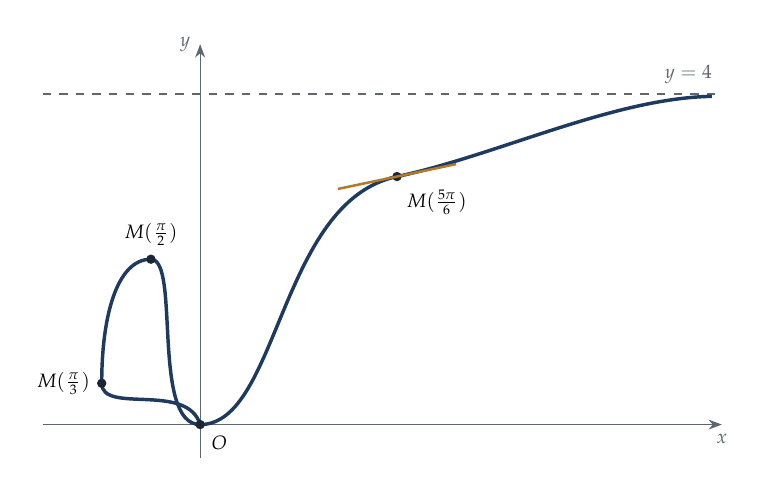
\begin{tikzpicture}[x=1.25cm,y=1.05cm,>=Stealth]
\draw[->,Gris] (-1.6,0)--(5.3,0) node[below]{\scriptsize$x$}; \draw[->,Gris] (0,-0.4)--(0,4.6) node[left]{\scriptsize$y$};
\draw[asy] (-1.6,4)--(5.3,4) node[above left]{\scriptsize$y=4$};
\draw[arcetude] (0,0) .. controls (-0.13,0.52) and (-1,0.12) .. (-1,0.5)
      .. controls (-1,1.3) and (-0.85,2) .. (-0.5,2)
      .. controls (-0.2,2) and (-0.5,0) .. (0,0)
      .. controls (0.8,0) and (0.8,2.7) .. (2,3)
      .. controls (3,3.25) and (4.2,3.95) .. (5.2,3.97);
\foreach \p in {(0,0),(-1,0.5),(-0.5,2),(2,3)} \node[pt] at \p {};
\node[font=\scriptsize,anchor=east] at (-1.02,0.5) {$M(\frac\pi3)$};
\node[font=\scriptsize,anchor=south] at (-0.5,2.05) {$M(\frac\pi2)$};
\node[font=\scriptsize,anchor=north west] at (2,2.95) {$M(\frac{5\pi}6)$};
\node[font=\scriptsize,anchor=north west] at (0.02,-0.02) {$O$};
\draw[tgte] (1.4,2.85)--(2.6,3.15);
\end{tikzpicture}
\end{center}
\q{2.} En $M\left(\frac{5\pi}6\right)=(2,3)$, $f'=(4,1)$ : $\det\big((x-2,y-3),(4,1)\big)=(x-2)-4(y-3)=0$, soit
\[x-4y+10=0\qquad\Big(y=\tfrac x4+\tfrac52\Big).\]
\q{3. Non.} Déjà $M\left(\frac{2\pi}3\right)=O$, mais $t=0$ est exclu ; il faut donc un argument plus fin. Sur
$\left]0,\frac\pi3\right]$, $x$ décroît de $0$ à $-1$ : l'arc $\Gamma_1$ est le graphe d'une fonction $h_1$ sur $[-1,0[$, à
valeurs dans $\left]0,\frac12\right]$. Sur $\left[\frac\pi3,\frac{2\pi}3\right]$, $x$ croît de $-1$ à $0$ : l'arc $\Gamma_2$ est le
graphe d'une fonction $h_2$ sur $[-1,0]$. Or :
\begin{itemize}
\item en $x=-\frac12$ : $h_2=2>\frac12\geq h_1$ ;
\item près de $0$ : $\Gamma_1$ part de $O$ avec la pente $-4$, donc $h_1(x)\sim-4x>0$ ; $\Gamma_2$ arrive en $O$ avec une tangente
      horizontale, donc $h_2(x)=o(x)$. Ainsi $h_1>h_2$ pour $x<0$ proche de $0$.
\end{itemize}
Par le théorème des valeurs intermédiaires appliqué à $h_1-h_2$ sur $\left[-\frac12,x\right]$, il existe $x_0\in\left]-\frac12,0\right[$
tel que $h_1(x_0)=h_2(x_0)$ : un point double, atteint par deux paramètres distincts de $]0,\pi]$. $g$ n'est pas injective.

\q{4. (i)} $f$ impaire : $M(-t)$ est le symétrique de $M(t)$ par rapport à $O$ (compatible avec $M(0)=O$). On ajoute l'image de
la courbe par la symétrie centrale ; la branche $t\to-\pi$ a l'asymptote $y=-4$, la courbe étant au-dessus.

\q{(ii)} $f$ $\pi$-périodique : $M(t-\pi)=M(t)$, la courbe sur $[-\pi,0[$ est parcourue une seconde fois, le dessin est le même.
Mais cette hypothèse est incompatible avec le tableau : elle imposerait $x(t)=x(t+\pi)\to+\infty$ quand $t\to0^-$, alors que $x$
est continue en $0$ avec $x(0)=0$.
\gain{pour prouver un point double sans calcul, on compare deux arcs écrits comme graphes ($x$ monotone) et l'on applique le
théorème des valeurs intermédiaires ; les pentes aux extrémités suffisent souvent.}
\piege{lire $x'(\frac\pi3)=0$ comme une tangente horizontale : c'est l'inverse ($x'=0$, $y'\neq0$ : verticale).}
\retenir{un tableau de variations conjoint contient toute l'information de tracé : points, tangentes, directions, asymptotes.
Avant d'utiliser une symétrie, vérifier sa compatibilité avec les valeurs connues.}
\end{corrige}
\begin{corrige}{td-c2}
\choix{lieu géométrique : on choisit le repère (le sol pour $(Ox)$, le mur pour $(Oy)$) et le paramètre imposé (l'angle) ;
« tangente » se traduit par une colinéarité, donc un déterminant nul.}
\q{1.} Soient $P$ le pied (sur $(Ox)$), $Q$ le sommet (sur $(Oy)$), $L=PQ$, et $M$ le barreau tel que $QM=a$, $MP=b$ ($L=a+b$).
Alors $P=(L\cos\theta,0)$, $Q=(0,L\sin\theta)$ et
$M=Q+\frac aL\vv{QP}=\big(a\cos\theta,(L-a)\sin\theta\big)=(a\cos\theta,b\sin\theta)$ : $M$ décrit un quart de l'ellipse
$\frac{x^2}{a^2}+\frac{y^2}{b^2}=1$ (un quart de cercle si $M$ est le milieu).

\q{2.} Valeurs pour $\theta=0,\frac\pi6,\frac\pi4,\frac\pi3,\frac\pi2$ : $(2,0)$, $\left(\sqrt3,\frac12\right)$,
$\left(\sqrt2,\frac{\sqrt2}2\right)$, $\left(1,\frac{\sqrt3}2\right)$, $(0,1)$ ; tangente verticale en $(2,0)$, horizontale en $(0,1)$.

\q{3.} L'échelle passe toujours par $M$ et est dirigée par $(\cos\theta,-\sin\theta)$ ; la courbe par
$M'(\theta)=(-a\sin\theta,b\cos\theta)\neq\ve0$. Tangence si et seulement si
\[\dt{-a\sin\theta&\cos\theta\\b\cos\theta&-\sin\theta}=a\sin^2\theta-b\cos^2\theta=0\iff\tan\theta=\sqrt{\tfrac ba}.\]
Pour $a=2$, $b=1$ : $\tan\theta=\frac1{\sqrt2}$, $\theta\approx35{,}3^\circ$, au point $M=\left(\frac{2\sqrt6}3,\frac{\sqrt3}3\right)$.
\begin{center}
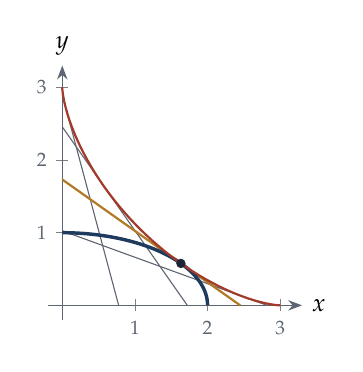
\begin{tikzpicture}
\begin{axis}[courbe,width=0.46\linewidth,xmin=-0.2,xmax=3.3,ymin=-0.2,ymax=3.3,xtick={1,2,3},ytick={1,2,3}]
\addplot[Gris,thin] coordinates {(2.819,0) (0,1.026)};
\addplot[Gris,thin] coordinates {(1.721,0) (0,2.457)};
\addplot[Gris,thin] coordinates {(0.776,0) (0,2.898)};
\addplot[Ocre,thick] coordinates {(2.449,0) (0,1.732)};
\addplot[arcetude,domain=0:1.5708,samples=100]({2*cos(x)},{sin(x)});
\addplot[Brique,thick,domain=0:1.5708,samples=100]({3*cos(x)^3},{3*sin(x)^3});
\node[pt] at (axis cs:1.633,0.577) {};
\end{axis}
\end{tikzpicture}
\end{center}
\gain{les positions de l'échelle sont toutes tangentes à l'astroïde $(L\cos^3\theta,L\sin^3\theta)$ (en brique), leur
\emph{enveloppe} (étudiée dans le volume \emph{Propriétés métriques et enveloppes}) ; la question 3 revient à chercher où l'ellipse et l'astroïde ont une tangente commune
le long de l'échelle.}
\retenir{lieu géométrique $\Rightarrow$ repère et paramètre naturels ; tangence $\Rightarrow\det(\text{vitesse},\text{direction})=0$.}
\end{corrige}
\begin{corrige}{td-c4}
\choix{dériver puis \emph{factoriser} : les dérivées sont des sommes de cosinus ou de sinus, que l'angle moitié transforme en
produits (signe immédiat).}
\q{1.} $f$ est $2\pi$-périodique, $x$ paire, $y$ impaire : axe $(Ox)$, étude sur $[0,\pi]$.

\q{2.} $e^{it}-e^{2it}=e^{\frac{3it}2}\left(e^{-\frac{it}2}-e^{\frac{it}2}\right)=-2i\sin\frac t2\,e^{\frac{3it}2}$, de partie réelle
$-2\sin\frac t2\,\mathrm{Re}\big(ie^{\frac{3it}2}\big)=2\sin\frac t2\sin\frac{3t}2$.

\q{3.} $x=\cos t-\cos^2t$ et $y=\sin t-\frac12\sin2t$, d'où
\[x'(t)=\sin t\,(2\cos t-1),\qquad y'(t)=\cos t-\cos2t=2\sin\tfrac t2\sin\tfrac{3t}2.\]
Sur $[0,\pi]$ : $x'\geq0$ sur $\left[0,\frac\pi3\right]$, $\leq0$ ensuite ; $y'>0$ sur $\left]0,\frac{2\pi}3\right[$, $<0$ ensuite.
\begin{center}
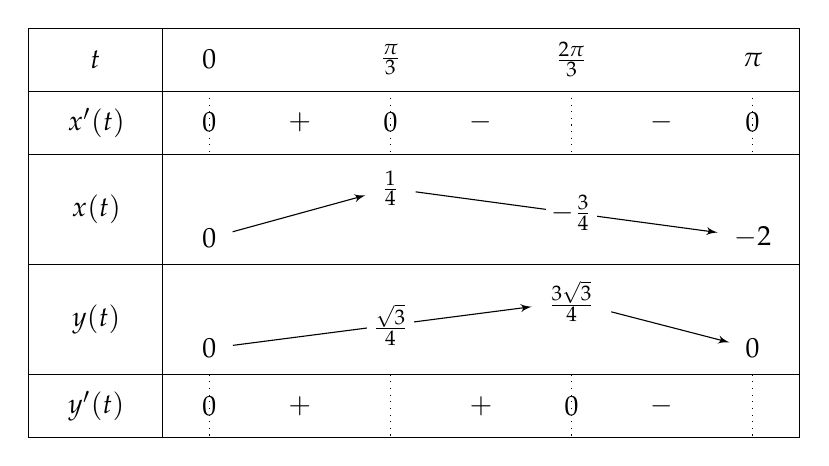
\begin{tikzpicture}
\tkzTabInit[lgt=1.7,espcl=2.3,deltacl=0.6]{$t$/0.8,$x'(t)$/0.8,$x(t)$/1.4,$y(t)$/1.4,$y'(t)$/0.8}{$0$,$\frac\pi3$,$\frac{2\pi}3$,$\pi$}
\tkzTabLine{z,+,z,-,t,-,z}
\tkzTabVar{-/$0$,+/$\frac14$,R/,-/$-2$}
\tkzTabIma{2}{4}{3}{$-\frac34$}
\tkzTabVar{-/$0$,R/,+/$\frac{3\sqrt3}4$,-/$0$}
\tkzTabIma{1}{3}{2}{$\frac{\sqrt3}4$}
\tkzTabLine{z,+,t,+,z,-,t}
\end{tikzpicture}
\end{center}
Tangente verticale en $\left(\frac14,\frac{\sqrt3}4\right)$ et en $(-2,0)$ ($f'(\pi)=(0,-2)$) ; horizontale en
$\left(-\frac34,\frac{3\sqrt3}4\right)$.

\q{4.} $f'(0)=\ve0$. Avec $1-\cos t=\frac{t^2}2+o(t^3)$ : $x=\frac{t^2}2+o(t^3)$, $y=\frac{t^2}2\cdot t+o(t^3)$, donc
$f(t)=t^2\left(\tfrac12,0\right)+t^3\left(0,\tfrac12\right)+o(t^3)$ : rebroussement de première espèce, tangente $(Ox)$, la courbe
arrivant du côté $x>0$. (À l'ordre 4, le terme $t^4\left(-\frac7{24},0\right)$ ne change rien : il est colinéaire
au premier.)

\q{5.} On place $O$ (pointe), les tangentes verticales et horizontale, on relie, puis on complète par symétrie d'axe $(Ox)$.
En polaire, $r=1-\cos\theta$ (\HP).
\begin{center}
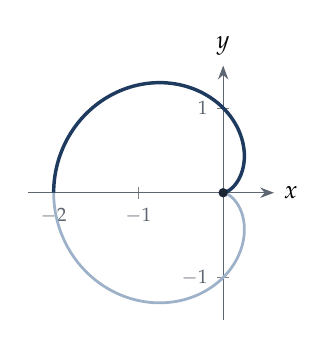
\begin{tikzpicture}
\begin{axis}[courbe,width=0.46\linewidth,xmin=-2.3,xmax=0.6,ymin=-1.5,ymax=1.5,xtick={-2,-1},ytick={-1,1}]
\addplot[reste,domain=-3.1416:0,samples=200]({(1-cos(x))*cos(x)},{(1-cos(x))*sin(x)});
\addplot[arcetude,domain=0:3.1416,samples=200]({(1-cos(x))*cos(x)},{(1-cos(x))*sin(x)});
\node[pt] at (axis cs:0,0) {};
\end{axis}
\end{tikzpicture}
\end{center}
\gain{$x'$ se factorise plus vite directement : $x'=-\sin t+2\cos t\sin t=\sin t(2\cos t-1)$. Choisir la factorisation la plus
courte, pourvu qu'elle donne le signe.}
\piege{en $t=\pi$, $x'=0$ mais $y'=-2\neq0$ : point régulier à tangente verticale, pas un point stationnaire.}
\retenir{$e^{ia}\pm e^{ib}=e^{i\frac{a+b}2}(\dots)$ : la factorisation par l'angle moitié est l'outil des dérivées
trigonométriques.}
\end{corrige}
\begin{corrige}{td-c6}
\choix{méthode~\ref{meth:inflexion} : $\det(f',f'')$, factorisé, puis étude du signe. Pour les branches, $\frac yx$.}
\q{1.} $x'(t)=\frac34(t-2)^2\geq0$, $y'(t)=2t$ : pas de point stationnaire ($x'=0$ seulement en $2$, où $y'=4$).
\begin{center}
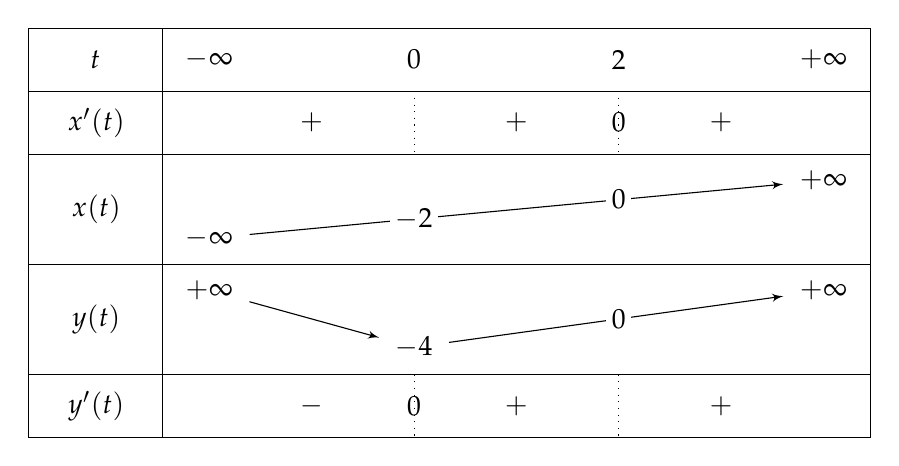
\begin{tikzpicture}
\tkzTabInit[lgt=1.7,espcl=2.6,deltacl=0.6]{$t$/0.8,$x'(t)$/0.8,$x(t)$/1.4,$y(t)$/1.4,$y'(t)$/0.8}{$-\infty$,$0$,$2$,$+\infty$}
\tkzTabLine{,+,t,+,z,+,}
\tkzTabVar{-/$-\infty$,R/,R/,+/$+\infty$}
\tkzTabIma{1}{4}{2}{$-2$}
\tkzTabIma{1}{4}{3}{$0$}
\tkzTabVar{+/$+\infty$,-/$-4$,R/,+/$+\infty$}
\tkzTabIma{2}{4}{3}{$0$}
\tkzTabLine{,-,z,+,t,+,}
\end{tikzpicture}
\end{center}
Tangente horizontale en $(-2,-4)$, verticale en $O$. Quand $t\to\pm\infty$, $\frac yx\sim\frac4t\to0$ : deux branches
paraboliques de direction $(Ox)$, \emph{aucune asymptote}.

\q{2.} $f''=\left(\frac32(t-2),2\right)$ et
\[\det(f',f'')=\frac32(t-2)^2-3t(t-2)=-\frac32(t-2)(t+2).\]
Il s'annule en $t=\pm2$ et change de signe en chacun (racines simples) : exactement deux points d'inflexion, $M(2)=O$ (tangente
verticale $x=0$) et $M(-2)=(-16,0)$, où $f'(-2)=(12,-4)$ donne la tangente $y=-\frac13(x+16)$.

\q{3.}
\begin{center}
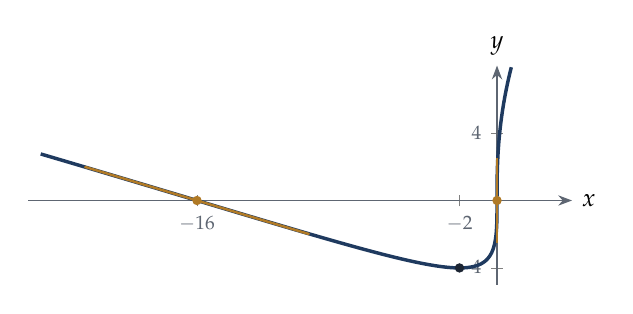
\begin{tikzpicture}
\begin{axis}[courbe,width=0.7\linewidth,height=0.36\linewidth,axis equal image=false,xmin=-25,xmax=4,ymin=-5,ymax=8,xtick={-16,-2},ytick={-4,4}]
\addplot[arcetude,domain=-2.6:3.45,samples=200]({(x-2)^3/4},{x^2-4});
\addplot[tgte,domain=-22:-10,samples=2]{-(x+16)/3};
\addplot[tgte,samples=2] coordinates {(0,-2.5) (0,2.5)};
\node[pt,fill=Ocre] at (axis cs:-16,0) {}; \node[pt,fill=Ocre] at (axis cs:0,0) {}; \node[pt] at (axis cs:-2,-4) {};
\end{axis}
\end{tikzpicture}
\end{center}
\gain{la pente $p(t)=\frac{y'}{x'}=\frac{8t}{3(t-2)^2}$ est minimale en $t=-2$ ($p=-\frac13$) : c'est l'inflexion, comme le prévoit
$p'=\frac{\det(f',f'')}{x'^2}$.}
\piege{une inflexion peut avoir une tangente verticale (ici en $O$) : elle ne se voit pas sur la pente, seulement sur le
déterminant.}
\retenir{« exactement deux » demande les deux sens : $\det=0$ (nécessaire) pour la liste des candidats, changement de signe
(suffisant) pour chacun.}
\end{corrige}
\begin{corrige}{td-c7}
\choix{développement en $t=\frac\pi2+h$ ; il faut aller \emph{loin} (ordre 5), car le terme en $h^3$ est nul et l'on doit
trouver le premier vecteur non colinéaire au premier.}
\q{1.} $\cos t=-\sin h$, $\sin t=\cos h$. Donc $x=1-\frac{h^2}2+\frac{h^4}{24}+o(h^5)$, $\cos^2t=\sin^2h=h^2-\frac{h^4}3+o(h^5)$,
$\cos^5t=-h^5+o(h^5)$ :
\[f\left(\tfrac\pi2+h\right)=(1,0)+h^2\left(-\tfrac12,\tfrac12\right)+h^4\left(\tfrac1{24},-\tfrac16\right)+h^5(0,-1)+o(h^5).\]
$\det\big((-\frac12,\frac12),(\frac1{24},-\frac16)\big)=\frac1{12}-\frac1{48}=\frac1{16}\neq0$ : $p=2$, $q=4$, rebroussement de
\emph{seconde} espèce en $(1,0)$, tangente dirigée par $(-1,1)$ : la droite $x+y=1$. Les deux arcs sont du côté de
$\ve b=\left(\frac1{24},-\frac16\right)$ ($h^4>0$), sous cette droite.

\q{2.} $x'=\cos t$ ; $y'=-5\cos^4t\sin t-\cos t\sin t=-\sin t\cos t\,(5\cos^3t+1)$, qui s'annule pour $\cos t=-5^{-1/3}$, soit
$t=\alpha\approx2{,}20$. Symétries : $f(-t)=(-x,y)$ : axe $(Oy)$ ; étude sur $[0,\pi]$.
Signes sur $[0,\pi]$ : $x'>0$ avant $\frac\pi2$, $<0$ après ; $y'<0$ sur $\left]0,\frac\pi2\right[$, $>0$ sur $\left]\frac\pi2,\alpha\right[$,
$<0$ sur $]\alpha,\pi[$. Points : $M(0)=\left(0,\frac32\right)$ et $M(\pi)=\left(0,-\frac12\right)$, tangentes horizontales (sur l'axe) ;
$M\left(\frac\pi2\right)=(1,0)$, rebroussement ; $A=M(\alpha)$ avec $\cos\alpha=-c$, $c=5^{-1/3}$ :
$A=\left(\sqrt{1-c^2},\ c^2\left(\frac12-c^3\right)\right)=\left(\sqrt{1-c^2},\ \frac3{10}c^2\right)\approx(0{,}81\,;0{,}10)$, tangente
horizontale.

\q{3.} Sur $[0,\pi]$ : de $\left(0,\frac32\right)$ vers la droite et le bas jusqu'à la pointe $(1,0)$, retour vers la gauche et le haut
jusqu'à $A$, puis vers la gauche et le bas jusqu'à $\left(0,-\frac12\right)$ ; on complète par symétrie d'axe $(Oy)$.
\begin{center}
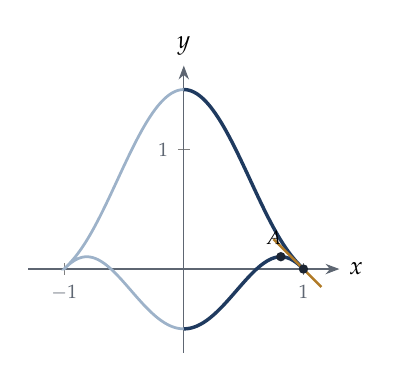
\begin{tikzpicture}
\begin{axis}[courbe,width=0.5\linewidth,xmin=-1.3,xmax=1.3,ymin=-0.7,ymax=1.7,xtick={-1,1},ytick={1}]
\addplot[reste,domain=-3.1416:0,samples=300]({sin(x)},{cos(x)^5+cos(x)^2/2});
\addplot[arcetude,domain=0:3.1416,samples=300]({sin(x)},{cos(x)^5+cos(x)^2/2});
\addplot[tgte,domain=0.75:1.15,samples=2]{1-x};
\node[pt] at (axis cs:1,0) {}; \node[pt] at (axis cs:0.811,0.103) {};
\node[font=\scriptsize,anchor=south] at (axis cs:0.75,0.12) {$A$};
\end{axis}
\end{tikzpicture}
\end{center}
\piege{s'arrêter à l'ordre 3 (aucun vecteur en $h^3$) ou à l'ordre 2 (on ne connaît que $\ve a$) : on ne peut pas conclure.
Il faut le « troisième » vecteur pour distinguer les deux espèces de rebroussement.}
\gain{$\cos^5t$ commence en $h^5$ : il est inutile de le développer plus loin, et inutile de développer $\cos^2t$ au-delà de $h^4$.}
\retenir{rebroussement de seconde espèce $\iff p$ et $q$ pairs : les deux arcs du même côté de la tangente.}
\end{corrige}
\begin{corrige}{td-c3}
\choix{suivre le plan d'étude ; pour la construction, paramétrer la droite $(OQ)$ par son angle, qui est le $\theta$ de l'énoncé.}
\q{1.} $f(\theta+\pi)=f(\theta)$ ($\sin^3$ et $\cos$ changent tous deux de signe) : période $\pi$. $x$ est impaire et $y$ paire :
$M(-\theta)$ est le symétrique de $M(\theta)$ par rapport à $(Oy)$, axe de symétrie. On étudie sur $\left[0,\frac\pi2\right[$.

\q{2.} $x'(\theta)=2a\frac{3\sin^2\theta\cos^2\theta+\sin^4\theta}{\cos^2\theta}=2a\frac{\sin^2\theta(2\cos^2\theta+1)}{\cos^2\theta}$ et
$y'(\theta)=2a\sin2\theta$. En $\frac\pi4$ : $M=(a,a)$, $f'=(4a,2a)$, direction $(2,1)$ :
$(x-a)-2(y-a)=0$, soit $T:x-2y+a=0$.

\q{3.} Sur $\left]0,\frac\pi2\right[$, $x'>0$ et $y'>0$ : $x$ croît de $0$ à $+\infty$, $y$ de $0$ à $2a$.

\q{4.} $x'=y'=0\iff\sin\theta=0$ : seul $M(0)=O$ (modulo $\pi$). À l'ordre 3 : $x=2a\theta^3+o(\theta^3)$, $y=2a\theta^2+o(\theta^3)$,
donc $f(\theta)=\theta^2(0,2a)+\theta^3(2a,0)+o(\theta^3)$ : $p=2$, $q=3$, rebroussement de première espèce en $O$, de tangente
$(Oy)$ ; la courbe est au-dessus de $O$ ($y\geq0$).

\q{5.} Quand $\theta\to\frac\pi2^-$ : $x\to+\infty$, $y\to2a$ : asymptote horizontale $\mathcal D:y=2a$. Comme $\sin^2\theta<1$, la courbe
est au-dessous. (Équation cartésienne, utile pour vérifier : $x^2(2a-y)=y^3$.)

\q{6.} $A=(0,2a)$ ; le cercle de diamètre $[OA]$ a pour équation $x^2+y^2=2ay$. Une droite issue de $O$ fait un angle $\theta$ avec
$(Oy)$ : elle est dirigée par $\ve u=(\sin\theta,\cos\theta)$. Le point $Q=r\ve u$ du cercle vérifie $r^2=2ar\cos\theta$, soit
$OQ=2a\cos\theta$ ; le point $H=r'\ve u$ de $\mathcal D$ vérifie $r'\cos\theta=2a$. D'où
\[\vv{OP}=\vv{QH}=\left(\frac{2a}{\cos\theta}-2a\cos\theta\right)\ve u=\frac{2a\sin^2\theta}{\cos\theta}(\sin\theta,\cos\theta)
=\left(2a\frac{\sin^3\theta}{\cos\theta},\,2a\sin^2\theta\right)=\vv{OM(\theta)}.\]
Quand $Q$ décrit le cercle, $\theta$ décrit $\left]-\frac\pi2,\frac\pi2\right[$ et $P$ décrit toute la cissoïde.
\begin{center}
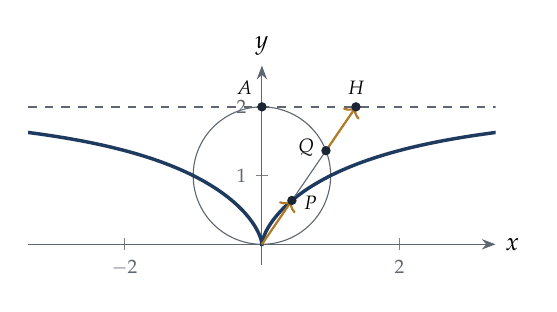
\begin{tikzpicture}
\begin{axis}[courbe,width=0.62\linewidth,xmin=-3.4,xmax=3.4,ymin=-0.3,ymax=2.6,axis equal image,xtick={-2,2},ytick={1,2}]
\addplot[asy,domain=-3.4:3.4,samples=2]{2};
\addplot[Gris,thin,domain=0:6.2832,samples=100]({cos(x)},{1+sin(x)});
\addplot[arcetude,domain=-1.13:1.13,samples=200]({2*sin(x)^3/cos(x)},{2*sin(x)^2});
\addplot[Gris] coordinates {(0,0) (1.368,2)};
\draw[->,Ocre,thick] (axis cs:0.932,1.362)--(axis cs:1.368,2);
\draw[->,Ocre,thick] (axis cs:0,0)--(axis cs:0.436,0.638);
\node[pt] at (axis cs:0.932,1.362) {}; \node[font=\scriptsize,anchor=east] at (axis cs:0.9,1.4) {$Q$};
\node[pt] at (axis cs:1.368,2) {}; \node[font=\scriptsize,anchor=south] at (axis cs:1.368,2.03) {$H$};
\node[pt] at (axis cs:0.436,0.638) {}; \node[font=\scriptsize,anchor=west] at (axis cs:0.47,0.6) {$P$};
\node[pt] at (axis cs:0,2) {}; \node[font=\scriptsize,anchor=south east] at (axis cs:0,2.03) {$A$};
\end{axis}
\end{tikzpicture}
\end{center}
\piege{l'axe de symétrie est $(Oy)$ et non $(Ox)$ : c'est $x$ qui est impaire. Ne pas plaquer le cas « usuel ».}
\gain{dans une construction issue de $O$, paramétrer chaque point par sa distance à $O$ sur la droite $O+\vect(\ve u)$ :
les équations deviennent des équations en $r$, immédiates.}
\retenir{la cissoïde réunit un rebroussement (DL à l'ordre 3), une asymptote horizontale et un lieu géométrique ; la méthode
« point courant $r\ve u$ » sert pour tous les lieux construits à partir d'un point fixe.}
\end{corrige}
\begin{corrige}{td-c5}
\choix{fractions rationnelles avec des puissances « miroirs » ($t$ et $t^3$ sur $1+t^4$) : tester $t\mapsto\frac1t$, qui échange
souvent $x$ et $y$.}
\q{Symétries.} $x\left(\frac1t\right)=\frac{1/t}{1+1/t^4}=\frac{t^3}{t^4+1}=y(t)$ et $y\left(\frac1t\right)=x(t)$ : $M(1/t)$ est le
symétrique de $M(t)$ par rapport à $y=x$, axe de symétrie. $f$ est impaire : symétrie de centre $O$. On étudie sur $[0,1]$ ;
$t\mapsto\frac1t$ donne $[1,+\infty[$, puis la symétrie centrale les $t<0$.

\q{Variations.} $x'(t)=\frac{1-3t^4}{(1+t^4)^2}$, $y'(t)=\frac{t^2(3-t^4)}{(1+t^4)^2}$. Sur $[0,1]$ : $y'\geq0$ ; $x'$ s'annule en
$t_1=3^{-1/4}\approx0{,}76$. Points : $M(0)=O$ avec $f'(0)=(1,0)$ (régulier, tangente horizontale) ;
$M(t_1)=\left(\frac34\,3^{-1/4},\frac34\,3^{-3/4}\right)\approx(0{,}57\,;0{,}33)$, tangente verticale ;
$M(1)=\left(\frac12,\frac12\right)$, $f'(1)=\left(-\frac12,\frac12\right)$ perpendiculaire à l'axe $y=x$ (point de raccord).

\q{Comportement en $\pm\infty$.} $M(t)\to O$ et $\frac yx=t^2\to+\infty$ : la courbe revient en $O$ tangentiellement à $(Oy)$
(c'est l'image par $y=x$ du départ horizontal en $t=0$). $O$ est donc un point double, de tangentes $(Ox)$ et $(Oy)$.

\q{Polaire.} $x^2+y^2=\frac{t^2(1+t^4)}{(1+t^4)^2}=\frac{t^2}{1+t^4}$ et $xy=\frac{t^4}{(1+t^4)^2}$, donc $(x^2+y^2)^2=xy$. Avec
$x=r\cos\theta$, $y=r\sin\theta$ : $r^4=r^2\cos\theta\sin\theta$, soit $r^2=\frac12\sin2\theta$ ($r\neq0$).
\begin{center}
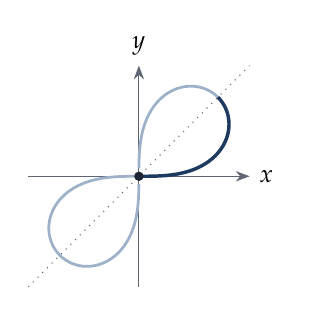
\begin{tikzpicture}
\begin{axis}[courbe,width=0.42\linewidth,xmin=-0.7,xmax=0.7,ymin=-0.7,ymax=0.7,xtick=\empty,ytick=\empty]
\addplot[Gris,dotted,domain=-0.7:0.7,samples=2]{x};
\addplot[reste,domain=-20:0,samples=600]({x/(1+x^4)},{x^3/(1+x^4)});
\addplot[reste,domain=1:20,samples=400]({x/(1+x^4)},{x^3/(1+x^4)});
\addplot[arcetude,domain=0:1,samples=100]({x/(1+x^4)},{x^3/(1+x^4)});
\node[pt] at (axis cs:0,0) {};
\end{axis}
\end{tikzpicture}
\end{center}
\piege{$O$ n'est atteint que pour $t=0$ ; le second passage est une \emph{limite} ($t\to\pm\infty$). Ne pas oublier ces limites
finies : elles ferment la courbe.}
\retenir{$t\mapsto\frac1t$ (et $t\mapsto-t$) réduisent l'étude à $[0,1]$ ; un point de l'axe de symétrie a une tangente
perpendiculaire à l'axe ; pour une équation polaire, partir de $x^2+y^2=r^2$.}
\end{corrige}
\begin{corrige}{td-c8}
\choix{même structure que la lemniscate (TD~5) : $t\mapsto\frac1t$ échange $x$ et $y$. Pour l'asymptote : méthode~\ref{meth:branches}
}
\q{1.} $x(1/t)=\frac{1/t}{1+1/t^3}=\frac{t^2}{t^3+1}=y(t)$ et $y(1/t)=x(t)$ : symétrie par rapport à $\Delta:y=x$. Comme $t\mapsto\frac1t$
échange $]-1,1[\setminus\{0\}$ et $]-\infty,-1[\cup]1,+\infty[$, l'étude sur $]-1,1[$ suffit.

\q{2.} $x'(t)=\frac{1-2t^3}{(1+t^3)^2}$, $y'(t)=\frac{t(2-t^3)}{(1+t^3)^2}$. Sur $]-1,1[$ : $x'$ s'annule en $t_1=2^{-1/3}$, $y'$ en
$0$. Quand $t\to-1^+$, $x\to-\infty$, $y\to+\infty$. $M(0)=O$, tangente horizontale ; $M(t_1)=\left(\frac23 2^{-1/3},\frac23 2^{-2/3}\right)
\approx(0{,}53\,;0{,}42)$, tangente verticale ; $M(1)=\left(\frac12,\frac12\right)$, tangente perpendiculaire à $\Delta$.

\q{3.} $\frac yx=t\to-1$ et $y+x=\frac{t(1+t)}{1+t^3}=\frac t{1-t+t^2}\to-\frac13$ (simplification par $1+t$) : asymptote
$\mathcal D:y=-x-\frac13$. Position :
\[y+x+\frac13=\frac{3t+1-t+t^2}{3(t^2-t+1)}=\frac{(t+1)^2}{3(t^2-t+1)}>0 :\]
la courbe est \emph{au-dessus} de $\mathcal D$, des deux côtés.
\begin{center}
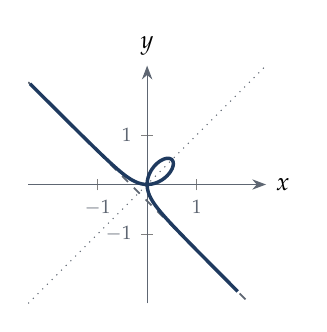
\begin{tikzpicture}
\begin{axis}[courbe,width=0.44\linewidth,xmin=-2.4,xmax=2.4,ymin=-2.4,ymax=2.4,xtick={-1,1},ytick={-1,1}]
\addplot[asy,domain=-2.4:2.4,samples=2]{-x-1/3};
\addplot[Gris,dotted,domain=-2.4:2.4,samples=2]{x};
\addplot[arcetude,domain=-0.86:40,samples=600]({x/(1+x^3)},{x^2/(1+x^3)});
\addplot[arcetude,domain=-40:-1.18,samples=300]({x/(1+x^3)},{x^2/(1+x^3)});
\end{axis}
\end{tikzpicture}
\end{center}
\gain{factoriser $1+t^3=(1+t)(1-t+t^2)$ dès le départ : la valeur interdite $-1$ et la simplification de $y+x$ apparaissent
aussitôt.}
\piege{conclure à l'asymptote avec $\frac yx\to-1$ seul : il faut $\lim(y+x)$.}
\retenir{position par rapport à une asymptote : mettre $y-(\alpha x+\beta)$ sur un dénominateur commun ; un carré au numérateur
signale que la courbe reste du même côté.}
\end{corrige}
\begin{corrige}{td-c9}
\choix{la question 4 se fait en premier (elle réduit le travail) ; le point $M(1)$ est sur l'axe, et la branche
$y\sim\frac{x^2}2$ appelle une comparaison avec la parabole $y=\frac{x^2}2$.}
\q{4 (d'abord).} $x(1/t)=\frac1t+\frac{t^2}2=y(t)$ et $y(1/t)=x(t)$ : le symétrique de $M(t)$ par rapport à $y=x$ est $M(1/t)$.

\q{1.} $x'=1-\frac1{t^3}$, $y'=t-\frac1{t^2}$ s'annulent en $t=1$ : $M(1)=\left(\frac32,\frac32\right)$ stationnaire. En $t=1+h$, avec
$(1+h)^{-2}=1-2h+3h^2-4h^3+o(h^3)$ et $(1+h)^{-1}=1-h+h^2-h^3+o(h^3)$ :
\[f(1+h)=\left(\tfrac32,\tfrac32\right)+h^2\left(\tfrac32,\tfrac32\right)+h^3(-2,-1)+o(h^3),\]
$\det\big((\frac32,\frac32),(-2,-1)\big)=\frac32\neq0$ : rebroussement de première espèce, de tangente la droite $y=x$ (l'axe). Les
deux arcs partent vers le haut à droite ; $\ve b=(-2,-1)$ vérifie $y-x=1>0$ : au-dessus de l'axe pour $h>0$, au-dessous pour
$h<0$ (ils sont symétriques).

\q{2.} $x'=\frac{t^3-1}{t^3}$, $y'=\frac{t^3-1}{t^2}$. Pour $t<0$ : $x'>0$, $y'<0$ ; pour $0<t<1$ : $x'<0$, $y'<0$ ; pour $t>1$ :
$x'>0$, $y'>0$. Limites : $t\to-\infty$ : $(-\infty,+\infty)$ ; $t\to0^-$ : $(+\infty,-\infty)$ ; $t\to0^+$ : $(+\infty,+\infty)$ ;
$t\to+\infty$ : $(+\infty,+\infty)$.

\q{3.} $x^2=t^2+\frac1t+\frac1{4t^4}$, donc $y-\frac{x^2}2=\frac1t-\frac1{2t}-\frac1{8t^4}=\frac1{2t}-\frac1{8t^4}\to0$ : la parabole
$y=\frac{x^2}2$ est asymptote quand $t\to\pm\infty$ (point de même abscisse), la courbe au-dessus pour $t\to+\infty$, au-dessous
pour $t\to-\infty$. Par symétrie, quand $t\to0^\pm$, la courbe est asymptote à la parabole $x=\frac{y^2}2$.
\begin{center}
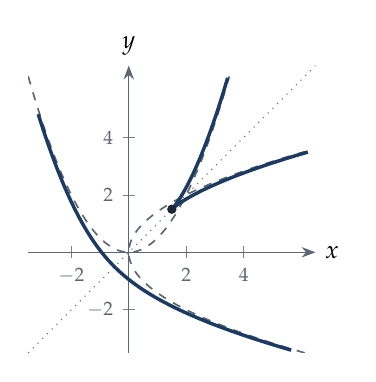
\begin{tikzpicture}
\begin{axis}[courbe,width=0.5\linewidth,xmin=-3.5,xmax=6.5,ymin=-3.5,ymax=6.5,xtick={-2,2,4},ytick={-2,2,4}]
\addplot[asy,domain=-3.5:3.5,samples=60]{x^2/2};
\addplot[asy,domain=-3.5:3.5,samples=60]({x^2/2},{x});
\addplot[Gris,dotted,domain=-3.5:6.5,samples=2]{x};
\addplot[arcetude,domain=-3.2:-0.29,samples=300]({x+1/(2*x^2)},{x^2/2+1/x});
\addplot[arcetude,domain=0.29:3.4,samples=300]({x+1/(2*x^2)},{x^2/2+1/x});
\node[pt] at (axis cs:1.5,1.5) {};
\end{axis}
\end{tikzpicture}
\end{center}
\gain{$\frac yx\to+\infty$ indique une branche parabolique de direction $(Oy)$ ; comme $y\sim\frac{t^2}2$ et $x\sim t$, on compare $y$ à
$\frac{x^2}2$ : la parabole précise la branche.}
\piege{une parabole asymptote n'est pas une asymptote au sens du programme (droite) : c'est une notion hors programme, que l'on
justifie par $M(t)P_t\to0$ avec un point $P_t$ explicite de la parabole.}
\retenir{un point stationnaire situé sur un axe de symétrie a pour tangente l'axe ou sa perpendiculaire ; les symétries
$t\mapsto\frac1t$ transforment les branches $t\to\infty$ en branches $t\to0$.}
\end{corrige}
\begin{corrige}{td-c10}
\choix{limites de $x$ et $y$ à chaque borne : infinies $\Rightarrow$ branche (méthode~\ref{meth:branches}) ; finies $\Rightarrow$
point limite, dont la tangente est la limite de la direction de la corde.}
\q{1.} Quand $t\to0$, $x$ et $y$ sont infinis du signe de $t$, et $\frac yx=\frac t{e^t-1}\to1$. Développement : $e^t-1=t\left(1+\frac t2+\frac{t^2}6+o(t^2)\right)$,
et $\frac1{1+u}=1-u+u^2+o(u^2)$ avec $u=\frac t2+\frac{t^2}6$ :
\[y=\frac1t\left(1-\frac t2+\frac{t^2}{12}+o(t^2)\right)=\frac1t-\frac12+\frac t{12}+o(t).\]
$y-x=-\frac12+\frac t{12}+o(t)$ : asymptote $\mathcal D:y=x-\frac12$ ; la courbe est au-dessus quand $t\to0^+$ ($x\to+\infty$),
au-dessous quand $t\to0^-$.

\q{2.} $t\to+\infty$ : $x\to0^+$, $y\sim e^{-t}\to0^+$ : $M(t)\to A=O$. Pente de la corde $\vv{AM(t)}$ : $\frac yx=\frac t{e^t-1}\to0$.
La courbe arrive en $O$ tangentiellement à $(Ox)$, par le quart de plan $x,y>0$.

\q{3.} $t\to-\infty$ : $x\to0^-$, $y\to-1$ : $M(t)\to B=(0,-1)$. $y+1=\frac{e^t}{e^t-1}<0$ et $\frac{y+1}x=\frac{te^t}{e^t-1}\to0$ :
tangente horizontale en $B$, la courbe arrivant par la gauche et par le bas.

\q{4.} $x'=-\frac1{t^2}<0$ et $y'=-\frac{e^t}{(e^t-1)^2}<0$ : sur chaque intervalle, le point va vers le bas et la gauche. Pour
$t<0$ : de $B$ (non atteint) vers $-\infty$ le long de $\mathcal D$ ; pour $t>0$ : de $+\infty$ le long de $\mathcal D$ jusqu'à $O$
(non atteint). Cohérence : avec $t=\frac1x$, le support est le graphe de $x\mapsto\frac1{e^{1/x}-1}$.
\begin{center}
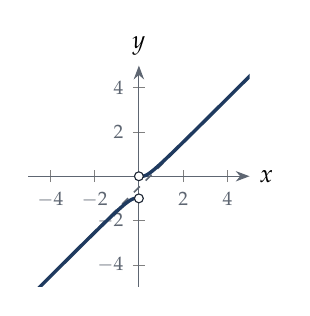
\begin{tikzpicture}
\begin{axis}[courbe,width=0.42\linewidth,xmin=-5,xmax=5,ymin=-5,ymax=5]
\addplot[asy,domain=-5:5,samples=2]{x-0.5};
\addplot[arcetude,domain=0.19:9,samples=300]({1/x},{1/(exp(x)-1)});
\addplot[arcetude,domain=-9:-0.205,samples=300]({1/x},{1/(exp(x)-1)});
\draw[Ink,fill=white] (axis cs:0,-1) circle (1.6pt);
\draw[Ink,fill=white] (axis cs:0,0) circle (1.6pt);
\end{axis}
\end{tikzpicture}
\end{center}
\gain{écrire $e^t-1=t(1+u)$ ramène le calcul à $\frac1{1+u}$ : c'est la manière la plus sûre de développer un inverse.}
\piege{oublier les bornes $t\to\pm\infty$ parce que les limites y sont finies : ce sont elles qui terminent la courbe (points
creux).}
\retenir{à chaque borne, d'abord $\lim x$ et $\lim y$ ; limite finie $\Rightarrow$ point limite et tangente $\lim\frac{y-y_A}{x-x_A}$ ;
la position se lit sur le premier terme non nul du développement asymptotique.}
\end{corrige}
\begin{corrige}{ds-pb}
\choix{chaque question réinvestit une méthode du livre (factorisation des dérivées, développement en $t_0\neq0$, position globale, asymptotes, courbe asymptote, inflexion par factorisation de la vitesse). On note les valeurs interdites dès le début : $-3$ (borne) et $0$.}

\textbf{1.(a)} $x'(t)=-\frac4{t^2}+\frac1{t+3}=\frac{t^2-4t-12}{t^2(t+3)}=\frac{(t-6)(t+2)}{t^2(t+3)}$ et
$y'(t)=1-\frac4{t^2}=\frac{(t-2)(t+2)}{t^2}$. Comme $t^2>0$ et $t+3>0$, les signes se lisent sur les facteurs affines. Limites et
valeurs : $x\to-\infty$, $y\to-\frac{13}3$ quand $t\to-3$ ; $M(-2)=(-2,-4)$ ($\ln1=0$) ; $x,y\to-\infty$ quand $t\to0^-$ et
$+\infty$ quand $t\to0^+$ ; $M(2)=(2+\ln5,\,4)$ ; $M(6)=\left(\frac23+\ln9,\,\frac{20}3\right)$ ; $x,y\to+\infty$ quand $t\to+\infty$.
\begin{center}
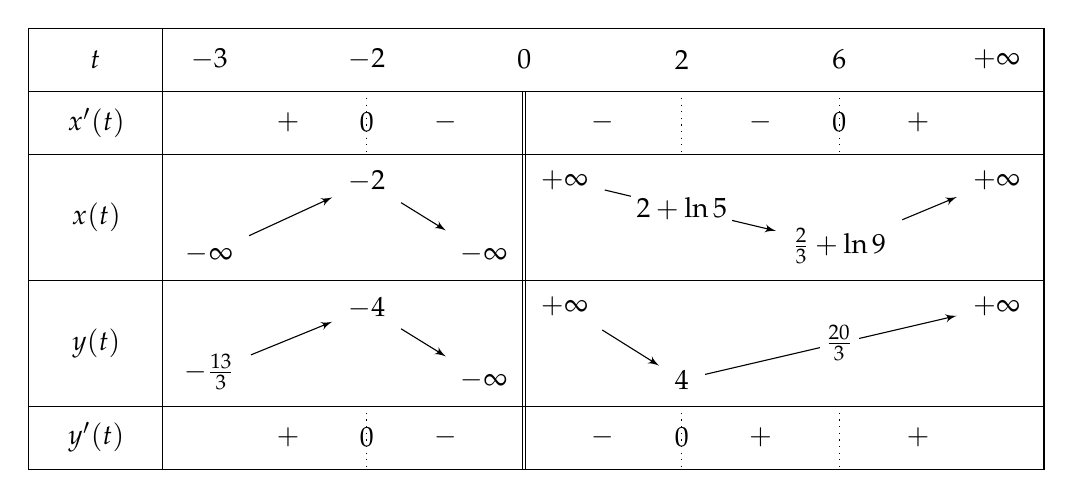
\begin{tikzpicture}
\tkzTabInit[lgt=1.7,espcl=2,deltacl=0.6]{$t$/0.8,$x'(t)$/0.8,$x(t)$/1.6,$y(t)$/1.6,$y'(t)$/0.8}{$-3$,$-2$,$0$,$2$,$6$,$+\infty$}
\tkzTabLine{,+,z,-,d,-,t,-,z,+,}
\tkzTabVar{-/$-\infty$,+/$-2$,-D+/$-\infty$/$+\infty$,R/,-/$\frac23+\ln9$,+/$+\infty$}
\tkzTabIma{3}{5}{4}{$2+\ln5$}
\tkzTabVar{-/$-\frac{13}3$,+/$-4$,-D+/$-\infty$/$+\infty$,-/$4$,R/,+/$+\infty$}
\tkzTabIma{4}{6}{5}{$\frac{20}3$}
\tkzTabLine{,+,z,-,d,-,z,+,t,+,}
\end{tikzpicture}
\end{center}

\textbf{(b)} Tangente verticale : $x'=0$ et $y'\neq0$, soit $t=6$ ($t=-2$ annule les deux) :
$A=M(6)=\left(\frac23+2\ln3,\frac{20}3\right)\approx(2{,}86\,;6{,}67)$. Tangente horizontale : $y'=0$, $x'\neq0$, soit $t=2$ :
$B=M(2)=(2+\ln5,4)\approx(3{,}61\,;4)$.

\textbf{(c)} Pour $t\notin\{-2,6\}$, $p(t)=\frac{y'(t)}{x'(t)}=\frac{(t-2)(t+2)}{t^2}\cdot\frac{t^2(t+3)}{(t-6)(t+2)}=\frac{(t-2)(t+3)}{t-6}$.
Alors $p(t)=m\iff t^2+t-6=m(t-6)\iff t^2+(1-m)t+6(m-1)=0$, de discriminant
$(1-m)^2-24(m-1)=(m-1)(m-25)$. Il est strictement négatif pour $1<m<25$ : aucune tangente n'a une pente dans $]1,25[$. Pour
$m=25$, la racine est double : $t=\frac{m-1}2=12$, qui est bien dans le domaine. D'où un unique point
$H=M(12)=\left(\frac13+\ln15,\frac{37}3\right)\approx(3{,}04\,;12{,}33)$.

\textbf{2.(a)} $\frac4{-2+h}=-\frac2{1-h/2}=-2-h-\frac{h^2}2-\frac{h^3}4+o(h^3)$ et $\ln(3+t)=\ln(1+h)=h-\frac{h^2}2+\frac{h^3}3+o(h^3)$.
D'où $x=-2-h^2+\frac{h^3}{12}+o(h^3)$, $y=-2+h+\frac4{-2+h}=-4-\frac{h^2}2-\frac{h^3}4+o(h^3)$ :
\[f(-2+h)=(-2,-4)+h^2\left(-1,-\tfrac12\right)+h^3\left(\tfrac1{12},-\tfrac14\right)+o(h^3).\]

\textbf{(b)} $\ve a=\left(-1,-\frac12\right)$ et $\ve b=\left(\frac1{12},-\frac14\right)$ ne sont pas colinéaires
($\det(\ve a,\ve b)=\frac14+\frac1{24}=\frac7{24}\neq0$) : $p=2$, $q=3$, $C$ est un point de \emph{rebroussement de première
espèce}. La tangente est dirigée par $\ve a$, ou par $(2,1)$ : $\det\big((x+2,y+4),(2,1)\big)=(x+2)-2(y+4)=0$, soit $x-2y=6$.

\textbf{(c)} Avec le développement : $\varphi(-2+h)=x-2y-6=-h^2+\frac{h^3}{12}+h^2+\frac{h^3}2+o(h^3)=\frac7{12}h^3+o(h^3)$.
La courbe traverse sa tangente en $C$ (rebroussement de première espèce) : elle est du côté $\varphi>0$, c'est-à-dire
\emph{au-dessous} de $T_C$ ($y<\frac{x-6}2$), pour $t$ un peu supérieur à $-2$, et au-dessus pour $t$ un peu inférieur.

\textbf{(d)} Méthode~\ref{meth:posglob} : $\varphi(t)=\ln(3+t)-2t-\frac4t-6$ et
\[\varphi'(t)=\frac1{t+3}-2+\frac4{t^2}=\frac{-2t^3-5t^2+4t+12}{t^2(t+3)}=-\frac{(t+2)^2(2t-3)}{t^2(t+3)}.\]
La racine double $-2$ était prévisible ($\varphi(-2)=\varphi'(-2)=0$ en un point de la tangente) et guide la factorisation.
Sur $]-3,0[$, $2t-3<0$ donc $\varphi'\geq0$ : $\varphi$ croît et s'annule en $-2$, d'où $\varphi<0$ sur $]-3,-2[$ et $\varphi>0$ sur
$]-2,0[$. Sur $]0,+\infty[$, $\varphi$ croît jusqu'en $\frac32$ puis décroît ; son maximum
$\varphi\left(\frac32\right)=\ln\frac92-\frac{35}3\approx-10{,}2$ est négatif : $\varphi<0$. Conclusion : $\mathcal C$ ne rencontre
$T_C$ qu'en $C$ ; elle est au-dessus de $T_C$ pour $t\in\,]-3,-2[\,\cup\,]0,+\infty[$ et au-dessous pour $t\in\,]-2,0[$, ce
qui prolonge l'étude locale.

\textbf{3.(a)} Quand $t\to0$, $x$ et $y$ sont infinis ; $\frac yx=\frac{t^2+4}{4+t\ln(3+t)}\to1$ et
$y-x=t-\ln(3+t)\to-\ln3$ : $\Delta_0:y=x-\ln3$ est asymptote. Position :
$y-x+\ln3=t-\ln\left(1+\frac t3\right)=\frac{2t}3+o(t)$ : au-dessus de $\Delta_0$ quand $t\to0^+$ (côté $x\to+\infty$),
au-dessous quand $t\to0^-$.

\textbf{(b)} Quand $t\to-3$, $x\to-\infty$ et $y\to-\frac{13}3$ : $\Delta':y=-\frac{13}3$ est asymptote horizontale. Comme $y$
est strictement croissante sur $]-3,-2]$, $y(t)>-\frac{13}3$ : la courbe est au-dessus de $\Delta'$.

\textbf{4.(a)} $x\sim\ln t$ et $y\sim t$, donc $\frac yx\to+\infty$ : branche parabolique de direction $(Oy)$.

\textbf{(b)} $e^{x(t)}=(3+t)\,e^{4/t}=(3+t)\left(1+\frac4t+\frac8{t^2}+O\!\left(\frac1{t^3}\right)\right)=t+7+\frac{20}t+O\!\left(\frac1{t^2}\right)$,
donc $\big(e^{x(t)}-7\big)-y(t)=\frac{16}t+O\!\left(\frac1{t^2}\right)\to0^+$. Le point $P_t=\big(x(t),e^{x(t)}-7\big)$ de
$\mathcal E$ vérifie $M(t)P_t\to0$ : $\mathcal E$ est asymptote, et la courbe est au-dessous.

\textbf{(c)} Le point de $y=e^x+c$ de même ordonnée est $Q_t=\big(\ln(y(t)-c),y(t)\big)$, et
$x(t)-\ln\big(y(t)-c\big)=\frac4t+\ln\frac{3+t}{t+\frac4t-c}\to0$ \emph{quel que soit} $c$. La distance horizontale ne
distingue aucune constante, alors que la distance verticale, $e^x+c-y\to7+c$, ne tend vers $0$ que pour $c=-7$. Pour une courbe
asymptote très pentue, on précise donc toujours quelle distance on utilise ; la plus exigeante est la distance verticale.

\textbf{5.(a)} $f'(t)=\lambda(t)\ve g(t)$ avec $\ve g(t)=\big(t-6,(t-2)(t+3)\big)=(t-6,t^2+t-6)$. Alors
$f''=\lambda'\ve g+\lambda\ve g'$ et, par bilinéarité, $\det(f',f'')=\lambda\lambda'\det(\ve g,\ve g)+\lambda^2\det(\ve g,\ve g')=\lambda^2\det(\ve g,\ve g')$.

\textbf{(b)} $\ve g'(t)=(1,2t+1)$ et $\det(\ve g,\ve g')=(t-6)(2t+1)-(t^2+t-6)=t^2-12t=t(t-12)$. En un point régulier
($t\neq-2$), $\lambda(t)\neq0$ : le seul candidat est $t=12$, et $\det(f',f'')$ change de signe en $12$ (racine simple, $\lambda^2>0$) :
$N=M(12)$ est l'unique point d'inflexion. C'est le point $H$ : d'après le \S2.4 ($p'=\frac{\det(f',f'')}{x'^2}$), la pente est extrémale en un
point d'inflexion à tangente non verticale. Ici $p$ décroît de $+\infty$ à $25$ sur $]6,12]$ puis croît : l'équation $p(t)=25$ a une
racine double en $12$.

\textbf{(c)} $T_N:y-\frac{37}3=25\left(x-\frac13-\ln15\right)$, soit $y=25x+12-25\ln15$.

\textbf{6.} On trace les asymptotes $\Delta_0$, $\Delta'$ et la courbe $\mathcal E$, on place $A$, $B$, $C$, $N$ avec leurs tangentes,
puis on suit le tableau : pour $t\in\,]-3,-2]$, la courbe vient de la gauche au-dessus de $\Delta'$ et monte jusqu'au
rebroussement $C$ ; elle repart vers le bas à gauche le long de $\Delta_0$ (au-dessous). Pour $t>0$, elle descend de l'infini le long
de $\Delta_0$ (au-dessus) jusqu'à $B$, remonte vers la gauche jusqu'à $A$, puis s'élève en traversant sa tangente en $N$ et longe
$\mathcal E$.
\begin{center}
\begin{tikzpicture}
\begin{axis}[courbe,width=0.86\linewidth,height=0.86\linewidth,axis equal image=false,xmin=-9,xmax=8,ymin=-10,ymax=14,
  xtick={-6,-2,2,6},ytick={-8,-4,4,8,12},restrict x to domain=-9:8,restrict y to domain=-10:14]
\addplot[asy,domain=-9:8,samples=2]{x-1.0986};
\addplot[asy,domain=-9:-1,samples=2]{-13/3};
\addplot[asy,domain=1.6:3.1,samples=60]{exp(x)-7};
\addplot[arcetude,domain=-2.99995:-0.42,samples=500]({4/x+ln(3+x)},{x+4/x});
\addplot[arcetude,domain=0.62:13.6,samples=500]({4/x+ln(3+x)},{x+4/x});
\addplot[tgte,domain=-4.5:0.5,samples=2]{(x-6)/2};
\addplot[tgte,samples=2] coordinates {(2.864,5.7) (2.864,7.6)};
\addplot[tgte,domain=2.9:4.3,samples=2]{4};
\addplot[tgte,domain=2.98:3.10,samples=2]{25*x+12-25*2.70805};
\node[pt] at (axis cs:-2,-4) {}; \node[font=\scriptsize,anchor=south east] at (axis cs:-2,-3.9) {$C$};
\node[pt] at (axis cs:2.864,6.667) {}; \node[font=\scriptsize,anchor=east] at (axis cs:2.8,6.667) {$A$};
\node[pt] at (axis cs:3.609,4) {}; \node[font=\scriptsize,anchor=north] at (axis cs:3.609,3.8) {$B$};
\node[pt,fill=Ocre] at (axis cs:3.041,12.333) {}; \node[font=\scriptsize,anchor=east] at (axis cs:2.95,12.333) {$N=H$};
\node[font=\scriptsize,Gris,anchor=west] at (axis cs:5.2,3.3) {$\Delta_0$};
\node[font=\scriptsize,Gris,anchor=south] at (axis cs:-7.5,-4.3) {$\Delta'$};
\node[font=\scriptsize,Gris,anchor=west] at (axis cs:3.12,14) {$\mathcal E$};
\end{axis}
\end{tikzpicture}
\end{center}
\retenir{le devoir enchaîne toujours les mêmes blocs : dérivées factorisées et tableau ; tangentes particulières (vérifier la
régularité) ; point stationnaire par développement en $t_0+h$ ; position locale puis globale ($\varphi$, racine double au point de
tangence) ; asymptotes à chaque valeur interdite et borne ; inflexion par factorisation de la vitesse ; dessin fidèle aux
positions.}
\end{corrige}
% =====================================================================
%                     INDEX DE CONSULTATION
% =====================================================================
\clearpage
\ongletsfalse
\section*{Index de consultation}\label{sec:index}
\addcontentsline{toc}{section}{Index de consultation}
\markboth{Index de consultation}{}

\subsection*{Correspondance avec le cours, les TD et le devoir}\phantomsection\label{sec:corresp}
{\footnotesize
\paragraph{Cours --- Déterminants}
\noindent Définition : linéarité, antisymétrie, $\det I_n=1$\dotfill th.~\ref{thm:def}, p.~\pageref{thm:def}\par
\noindent Développement, mineurs $\Delta_{i,j}$, définition par récurrence\dotfill th.~\ref{thm:dev}, p.~\pageref{thm:dev}\par
\noindent Aire orientée, $\|\ve u\|\|\ve v\|\sin(\ve u,\ve v)$, inverse $2\times2$\dotfill p.~\pageref{prop:col}\par
\noindent Volume, produit mixte\dotfill p.~\pageref{eq:det3}\par
\noindent Matrice triangulaire (preuve par récurrence), pivot, exemple $4\times4$\dotfill th.~\ref{thm:tri}, p.~\pageref{thm:tri}\par
\noindent Comatrice \HP\dotfill p.~\pageref{hp:comatrice}, ex.~\ref{e:hp-com}\par
\noindent $\det(AB)$, $\det(\lambda A)$, $\det A^{-1}$, $\det A^T$, bases, $\det f$, matrices semblables\dotfill p.~\pageref{thm:fond}\par
\noindent Projecteurs et symétries\dotfill prop.~\ref{prop:proj-sym}\par
\noindent Matrices $\max(i,j)$ et $|i-j|$\dotfill ex.~\ref{ex:max}, ex.~\ref{e:f-absij}\par
\paragraph{TD --- Déterminants}
\noindent 1.~Alignement \dotfill ex.~\ref{e:td-d1}\quad 2.~Distance de deux droites\dotfill ex.~\ref{e:td-d2}\par
\noindent 3.~Récurrence d'ordre 2 \dotfill ex.~\ref{e:td-d3}\quad 4.~Déterminant en X\dotfill ex.~\ref{e:td-d4}\par
\noindent 5.~Vandermonde \dotfill ex.~\ref{e:td-d5}\quad 6.~Base et déterminant\dotfill ex.~\ref{e:td-d6}\par
\noindent 7.~Récurrence, $2\cos\theta$ \dotfill ex.~\ref{e:td-d7}\quad 8.~Similitude \HP\dotfill ex.~\ref{e:td-d8}\par
\noindent 9.~Déterminant en Z \dotfill ex.~\ref{e:td-d9}\quad 10.~Polynôme de degré 1\dotfill ex.~\ref{e:td-d10}\par
\paragraph{Cours --- Courbes paramétrées}
\noindent Équation cartésienne et représentation paramétrique\dotfill p.~\pageref{sec:courbes}\par
\noindent Tangente (vecteur unitaire), preuve par Taylor--Young, équation, pente\dotfill th.~\ref{thm:tgte}, p.~\pageref{thm:tgte}\par
\noindent Plan d'étude ; ellipse\dotfill méth.~\ref{meth:plan-courbe}\par
\noindent Quatre allures, $(t^p,t^q)$, théorème et preuve, point anguleux\dotfill th.~\ref{thm:pq}, p.~\pageref{thm:pq}\par
\noindent Exemple $\big(t-2\sqrt{1+t},t\ln(1-t)\big)$ ; cardioïde en $O$\dotfill méth.~\ref{meth:dl}, ex.~\ref{e:td-c4}\par
\noindent Point birégulier, inflexions\dotfill méth.~\ref{meth:inflexion}\par
\noindent Asymptote, distance point--droite, folium\dotfill méth.~\ref{meth:branches}, ex.~\ref{e:td-c8}\par
\noindent Lissajous : point double, intersection, inflexions\dotfill ex.~\ref{ex:liss}, p.~\pageref{ex:liss}\par
\paragraph{TD --- Courbes paramétrées}
\noindent 1.~Tableau de variation \dotfill ex.~\ref{e:td-c1}\quad 2.~Ellipse et échelle\dotfill ex.~\ref{e:td-c2}\par
\noindent 3.~Cissoïde \dotfill ex.~\ref{e:td-c3}\quad 4.~Cardioïde\dotfill ex.~\ref{e:td-c4}\par
\noindent 5.~Lemniscate \HP\dotfill ex.~\ref{e:td-c5}\quad 6.~Points d'inflexion\dotfill ex.~\ref{e:td-c6}\par
\noindent 7.~Bicorne \dotfill ex.~\ref{e:td-c7}\quad 8.~Cubique de Descartes\dotfill ex.~\ref{e:td-c8}\par
\noindent 9.~Axe oblique, parabole \HP\dotfill ex.~\ref{e:td-c9}\quad 10.~Asymptote et prolongement\dotfill ex.~\ref{e:td-c10}\par
\paragraph{Devoir surveillé}
\noindent Tangentes particulières, DL en $t_0\neq0$, position locale et globale, asymptotes, courbe asymptote \HP, inflexion
par $\vec g=\lambda f'$, dessin\dotfill pb.~\ref{e:ds-pb}, méth.~\ref{meth:posglob}, \ref{meth:inflexion}\par
}

\subsection*{Méthodes}
{\footnotesize\begin{multicols}{2}\listemethodes\end{multicols}}

\end{document}
